\chapter{Experiments \& Results}\label{ch:results}

Given a parameterized framework for generating instances of resource exchanges,
experiments are designed and executed to explore the efficiency and quality of
solutions provided by different solvers. 

\S \ref{results:setup} describes the experimentation apparati, including the
computational tools, solvers and relevant output. Two experimental campaigns
were conducted. A scaling campaign, described in \S \ref{results:scale}, was
performed in order to investigate formulation behavior as a function of problem
size. \S \ref {results:stochastic} then describes the results of a stochastic
campaign.


\section{Experimental Setup}\label{results:setup}

An experiment consists of a set of resource-exchange graph instances executed
with a collection of configured solvers. When a solution is found, the solution
(i.e., the flow vector), the time required to reach the solution, and the
objective value (i.e., the dot-product of cost and flow vectors) are
recorded. Because solution time is a quantity of interest, all instances in an
experiment must be executed on homogeneous architecture. Furthermore, all
experiments must be executed on equivalent, homogeneous architecture in order to
quantify valid comparisons in solutions times across experimental campaigns.

Six execution nodes on UW-Madison Advanced Computing Initiative (ACI) HTCondor
system form the homogeneous environment used to conduct the experiments herein
described. Each execute node is comprised of an 2.90 GHz eight-core,
sixteen-thread, Intel Xeon E5-2690 \cite{intelproc} processor with 128 GB of
RAM. Processor hyper-threading was disabled for the duration of the experimental
campaign to allow comparisons between solution times.

For each experimental study, an input database consisting of persisted resource
exchange graph instances is generated. A copy of the database is transferred
from a user's submit node to each of the six execution nodes. A WorkQueue master
process is initiated. Sixteen workers per node are initialized using WorkQueue's
\texttt{condor\_submit\_workers} CLI. The master maintains a queue of instances
to be solved, assigning instances to workers as workers become available. Upon
completion, the input database is removed from each execution node, and the
results are collected from the user's submit node. The resulting database is
then post-processed and analyzed.

\subsection{Solvers and Formulations}

Three solvers are executed for each resource exchange graph instance: the Greedy
Heuristic, described in \S \ref{abm:dre:nfctp:heur}, COIN's LP solver
(COIN-CLP), and COIN's branch-and-cut solver (COIN-CBC). Each problem instance
is constructed as a \texttt{ExchangeGraph}, i.e., at the \textit{exchange layer}
shown in Figure \ref{fig:dre_impl} and Figure \ref{fig:dre_time}. The Greedy
Heuristic is applied directly to the \texttt{ExchangeGraph}. The CLP and CBC
solvers require a translation to the \textit{formulation layer}. The CLP solver
is applied to the LP formulation of the NFCTP and the CBC solver is applied to
the MILP formulation. The solution time, $t_s$ of a given solver is defined as
the time required to return a vector of arc flows given an
\texttt{ExchangeGraph} instance as shown in Figure \ref{fig:dre_time}.

\begin{equation}\label{eqn:solnt}
t_s = t_f - t_i
\end{equation}

\begin{figure}
  \begin{center}
    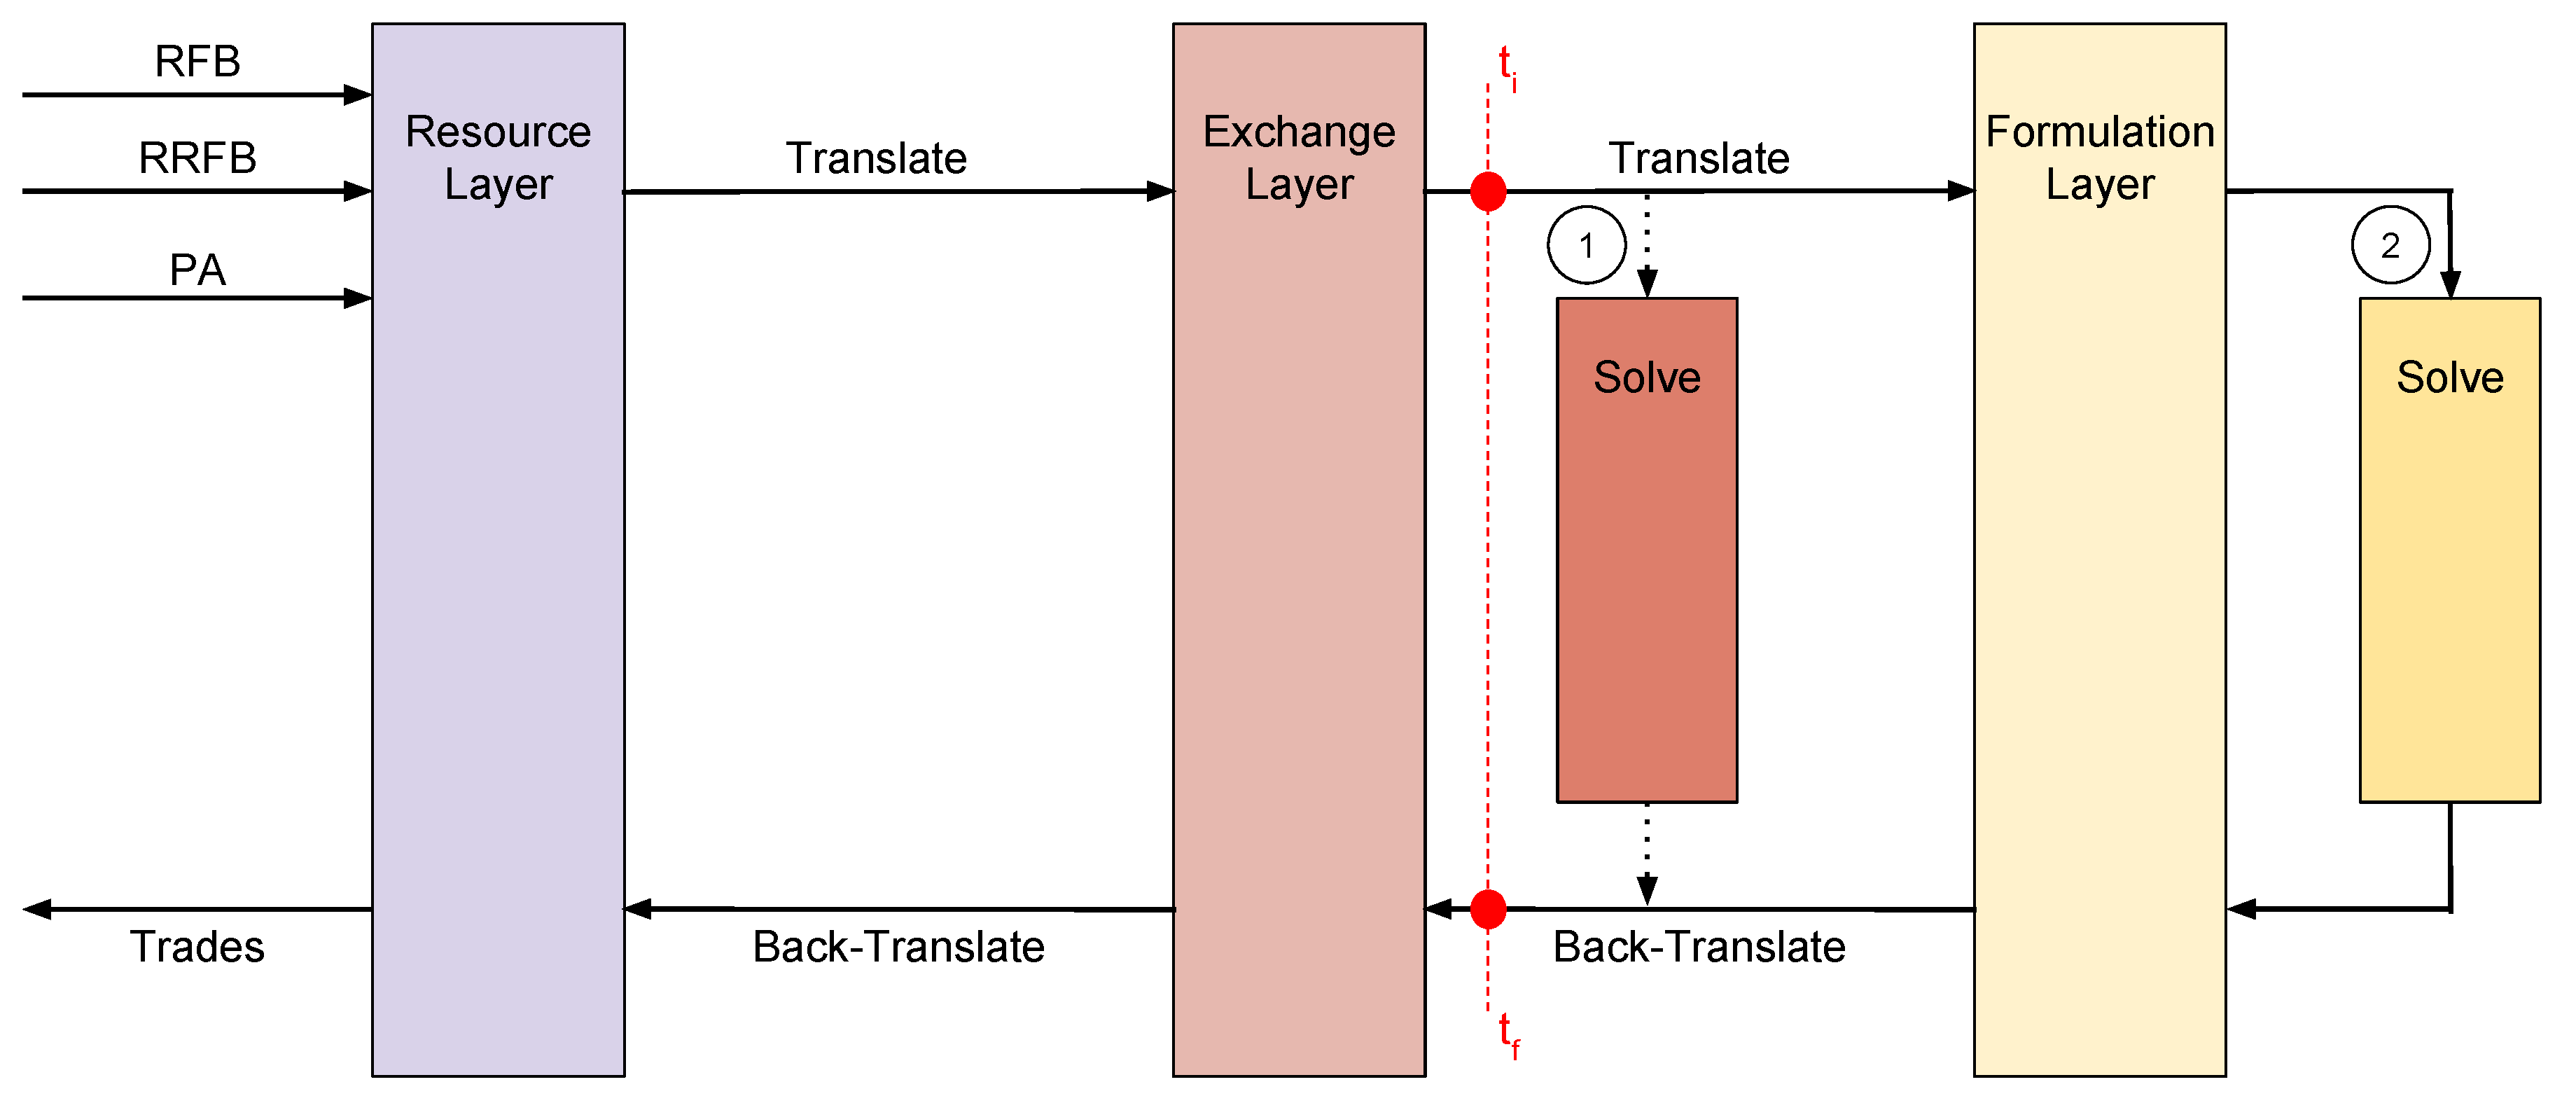
\includegraphics[width=\textwidth]{exchange_xlation_timing.pdf}
    \caption[]{
      \label{fig:dre_time}
      The time points for comparing different solutions using Equation \ref{eqn:solnt}.}
  \end{center}
\end{figure}

The Greedy Heuristic has $\mathcal{O}(N_A)$ scaling, where $N_A$ is the number
of arcs in the system. In the worst case, i.e., in highly constrained systems,
every arc will be processed. As both CLP and CBC solve NP-Hard problems, there
is no \textit{a priori} expected performance behavior.

\subsection{Parameter Variation}

\S \ref{method:setup:params} describes the parameters defining both Front and
Back-End exchanges. Each combination of fundamental parameters represents a
significant modeling assumption. Therefore, every experiment is conducted for
every combination of fundamental parameters, comprising eighteen combinations in
total. For exchange type, a reference instance parameter vector is
chosen. Experiments, then, are conducted by using either the reference vector or
perturbing instance parameter values from the reference vector and comparing
output.

Reference instance parameter vectors for front and back-end exchanges are shown
in Tables \ref{tbl:front_ref_params} and \ref{tbl:back_ref_params},
respectively. Reactor population and core composition values were chosen in line
with what a user might reasonably find in a simulation, such as a 75\%-25\%
thermal-to-fast reactor split and 33\% possible MOX-fuel residency in thermal
reactors. Support facility population values were chosen to model a ``worst
case'' simulation. The notion of a ``worst case'' simulation is defined as one
in which supporting facilities' services do not fully meet the demand of the
reactor population. Therefore, the resulting exchanges are highly constrained,
resulting in ``worst case'' behavior for the Greedy Heuristic. 

\begin{table}[h!]
\centering
\caption{Reference Values for Front-End Exchange Instance Parameters.}
\label{tbl:front_ref_params}
\begin{tabular}{|c|c|}
\hline
Parameter    & Reference Value
\\ \hline
$r_{rx, \text{Th}}$   & 0.75 
\\ \hline
$r_{rx, \text{FThOX}}$ & 0.25
\\ \hline
$r_{l, c}$ & 1
\\ \hline
$f_{mox}$     & 0.33
\\ \hline
$r_{s, \text{Th}}$ & 0.08
\\ \hline
$r_{s, \text{TMOX}, \text{UOX}}$ & 1.
\\ \hline
$r_{s, \text{FMOX}}$ & 0.2
\\ \hline
$r_{s, \text{FThOX}}$ & 0.2
\\ \hline
$r_{inv, proc}$   & 1
\\ \hline
\end{tabular}
\end{table}

\begin{table}[h!]
\centering
\caption{Reference Values for Back-End Exchange Instance Parameters.}
\label{tbl:back_ref_params}
\begin{tabular}{|c|c|}
\hline
Parameter    & Reference Value
\\ \hline
$r_{rx, \text{Th}}$   & 0.75 
\\ \hline
$r_{rx, \text{FThOX}}$ & 0.25
\\ \hline
$r_{l, c}$ & 1
\\ \hline
$f_{mox}$     & 0.33
\\ \hline
$r_{s, \text{Th}}$ & 0.08
\\ \hline
$r_{s, \text{TMOX}, \text{UOX}}$ & 1.
\\ \hline
$r_{s, \text{FMOX}}$ & 0.2
\\ \hline
$r_{s, \text{FThOX}}$ & 0.2
\\ \hline
$r_{s, \text{Repo}}$   & 0.2
\\ \hline
$d_{\text{Th}}$   & {UOX: 2/3, TMOX: 1/3, FMOX: 0}
\\ \hline
$d_{\text{FMOX}}$   & {UOX: 1/4, TMOX: 0, FMOX: 3/4, FThOX: 0}
\\ \hline
$d_{\text{FThOX}}$   & {UOX: 1/4, TMOX: 0, FMOX: 0, FThOX: 3/4}
\\ \hline
\end{tabular}
\end{table}

\subsection{Analysis Metrics}

The most obvious metrics to compare between solutions is the solution time,
$t_s$, and objective function value $z$,

\begin{equation}\label{eqn:obj_flow}
z = \sum_{(i, j) \in A} c_{i, j} x_{i, j}.
\end{equation}

For any given instance, the optimal objective value, $z^*$, is associated with a
set of flows, $x^*$. By definition, an optimal solution will have a lower or
equivalent system cost than any feasible solution.

While the objective function is minimized in the NFCTP formulations, it
necessarily includes flow along false arcs. Considering all arcs that exist both
in the formulation and the simulation, $A_{\text{sim}}$, another valid
comparison is dot product of preference and flow vectors. This value can be
considered the ``simulation objective'', i.e.,

\begin{equation}\label{eqn:sim_flow}
z_{\text{sim}} = \sum_{(i, j) \in A_{\text{sim}}} p_{i, j} x_{i, j}.
\end{equation}

A similar guarantee cannot be provided for $z^*_{\text{sim}}$. That is, while
$z^* \leq z$ is true in cost space, $z^*_{\text{sim}} \geq z_{\text{sim}}$ is
\textit{not} necessarily true.

%% The preference vector, $\vec{p}$, can be divided into its two components,
%% $\vec{p} = \vec{p}_c + \vec{p}_l$. If $f_{\text{loc}}$ is zero, then, by
%% definition, $\vec{p}_l = 0$, otherwise, it is comprised of non-zero
%% components. $\vec{p}_c$, however, is invariant under all values of
%% $f_{\text{loc}}$. Therefore, the commodity contribution of the simulation
%% objective, shown in Equation \ref{eqn:cpref_flow} is also an interesting
%% metric. It allows for direct investigation of the effect of adding
%% location-based preferences to the system. Furthermore, comparisons can be made
%% between systems with coarse and fine location-based preferences using this
%% metric.

%% \begin{equation}\label{eqn:cpref_flow}
%% z^c_{\text{sim}} = \sum_{(i, j) \in A_{\text{sim}}} p^c_{i, j} x_{i, j}.
%% \end{equation}

Each of the above metrics compare aggregate values between solutions. That is,
comparisons are being made at a macroscopic scope. For any two solutions to
identical problem instances, though, more detailed comparisons can be made. The
individual flow values, and values derived therefrom, can be compared directly
using a well-known normative measure. One example is the root mean square (RMS)
of constituents of the objective function, shown in Equation
\ref{eqn:rms_flow}.

\begin{equation}\label{eqn:rms_flow}
RMS_{\text{z}} = \sqrt{ \frac{1}{N} \sum_i c_i^2 (x_{i, 1} - x_{i, 2}) ^2 }
\end{equation}

While such an analysis is common in the realm of nuclear engineering, it is less
appropriate for comparing solutions to optimization problems. An instance of an
optimization problem may be \textit{degenerate}, i.e., it may have multiple
equivalent optimal solutions. Consider a two-arc system with arc costs of unity
and a total flow constraint of unity. A spectrum equivalent solutions exist
between $(0, 1)$ and $(1, 0)$. When comparing any solution, the difference in
objective function value is, necessarily, zero. However, using an RMS analysis,
the solutions of $(0, 1)$ and $(1, 0)$ would report the largest possible
error. Therefore, only metrics that involve aggregate measures of solutions are
used in the following analysis.



\section{Scalability Campaign}\label{results:scale}

Given the base parameter values described in Tables \ref{tbl:front_ref_params}
and \ref{tbl:back_ref_params}, exchanges were generated by scaling the number of
reactors in the system. The smallest system modeled included five reactors. The
largest exchanges included five-hundred reactors, a value chosen because there
are approximately five-hundred reactors currently operating (437) or under
construction (71) in the world \cite{nrxtrs}. Therefore, the largest exchanges
modeled represent a time step in a simulation in which the world-wide fleet of
reactors are all supplying or consuming a batch of fuel.

Front and back-end exchanges are explored similarly in the scalability
campaign. First, for all 18 combinations of fundamental parameters and each
solver, a set of reference cases are established, where the only varying
parameter is the number of reactors. Next, specific instance parameters are
chosen to vary in order to determine first-order effects as the exchange system
size scales. Finally, the effect of convergence criteria for the CBC solver is
investigated.

Individual figures for each experiment are provided for each fuel cycle modeled
($f_\text{fc}$) and each solver. Each figure summarizes the results for all
combinations of $f_\text{rx}$ and $f_\text{loc}$. The layout for each six-pane
figure is shown below.

\begin{figure}[h!]
  \begin{center}
    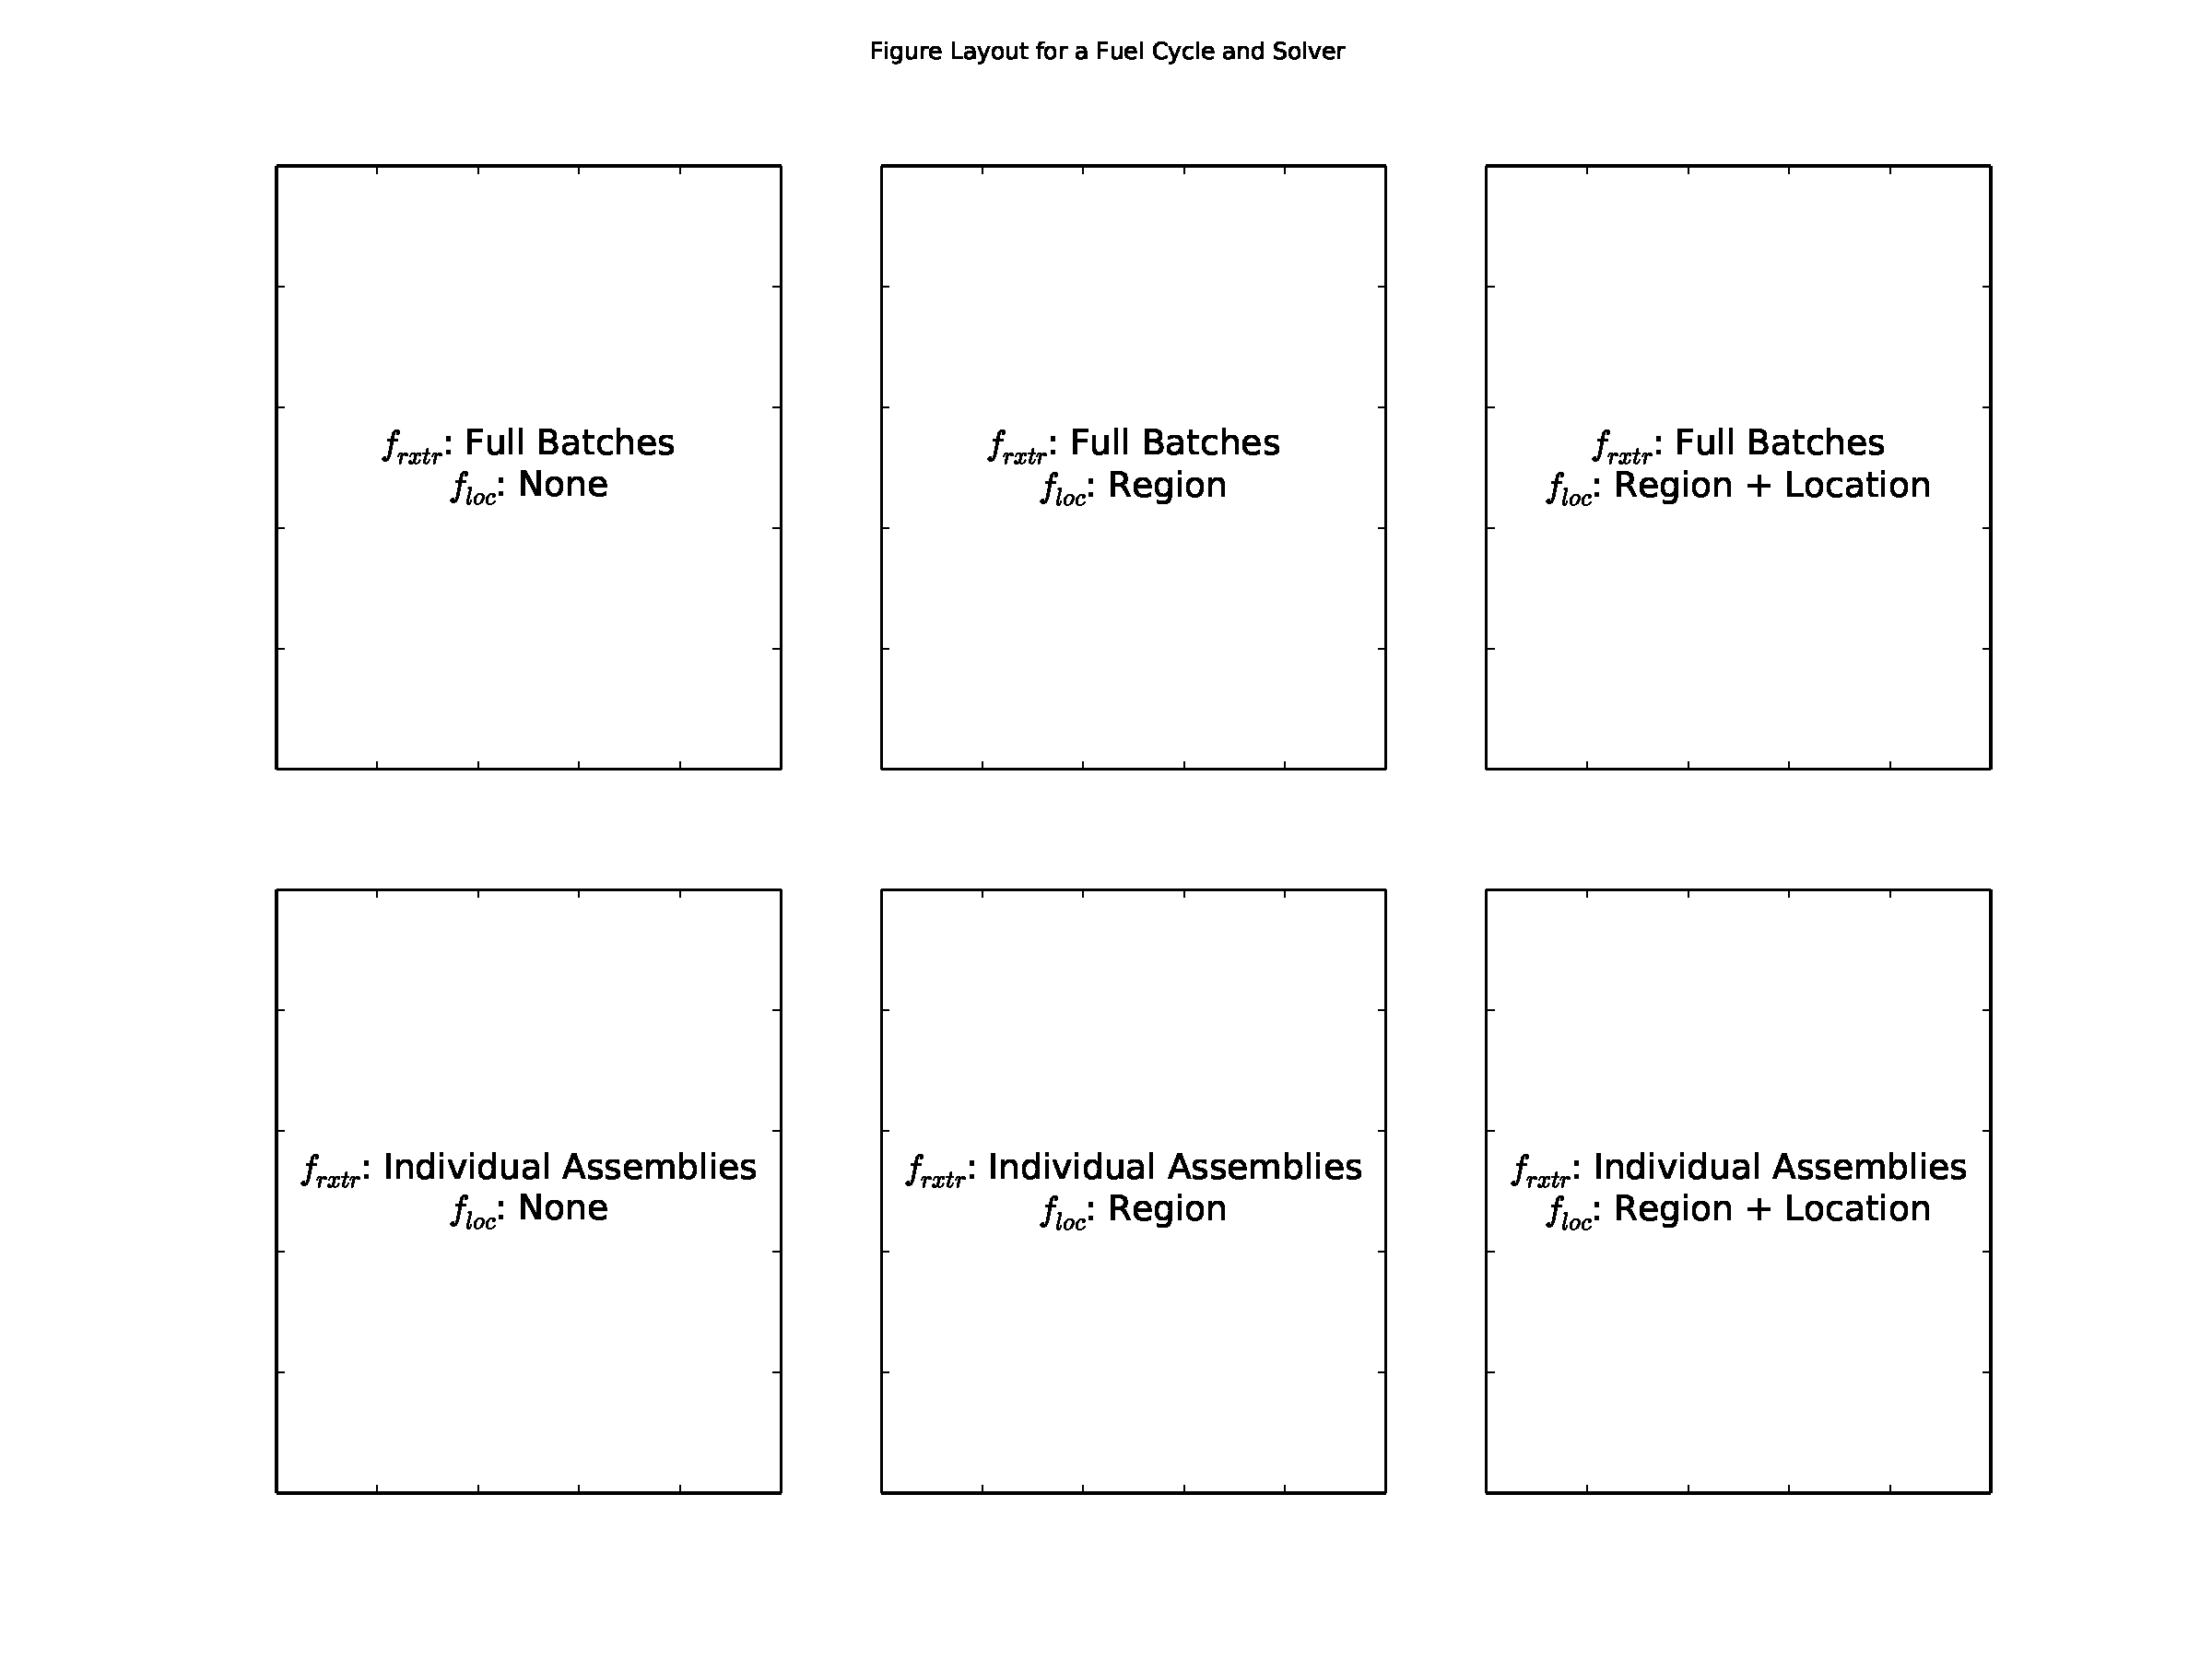
\includegraphics[width=.7\textwidth]{figure_layout.pdf}
    \caption[]{
      \label{fig:figure_layout}
      The general figure layout displaying results for different fundamental
      parameter values.}
  \end{center}
\end{figure}

\subsection{Front-End Exchanges}

\subsubsection{Reference Case}

Reference cases were generated for front-end exchanges by scaling the number of
reactors in each exchange. A step size of 5 reactors was used for the range of
$[5, 100]$ and a step size of 25 was used from $(100, 500]$. In mathematical
  programming, the number of variables and number of constraints in a problem
  are measures of problem scaling. In the NFCTP, constraints are provided by
  trading entities, and the number of variables is equal to the number of arcs
  in a given exchange graph. Accordingly, understanding how each quantiy scales
  with the number of reactors is of chief import.

Figure \ref{fig:base_front_n_rxtr_n_arcs_fc1_solvergreedy} shows how the number
of arcs scale with problem size for the MOX fuel cycle, and Figure
\ref{fig:base_front_n_rxtr_n_constrs_fc1_solvergreedy} shows the same results
for the number of constraints. The number of constraints scales linearly, for it
is a purely function of the number of entities in an exchange. However, the
number of arcs scales by $\mathcal{O}(n^2)$. During exchange generation, the
number of suppliers is a function of the number of reactors. Further, each
reactor and each supplier have an arc connecting them if the reactor can consume
the supplier's commodity. Therefore, adding a single reactor to the system
results in additional arcs for every reactor previously existing in the system,
resulting in an $\mathcal{O}(n^2)$ relationship. Both relationships hold true
regardless of the fuel cycle being modeled, and, as can be seen, are also
independent of other fundamental parameters. The arc population magnitude,
however, is a function of $f_\text{rxtr}$. As $f_\text{rxtr}$ increases, $n_a$
individual assemblies are requested rather than a single batch.

\begin{figure}[h!]
  \begin{center}
    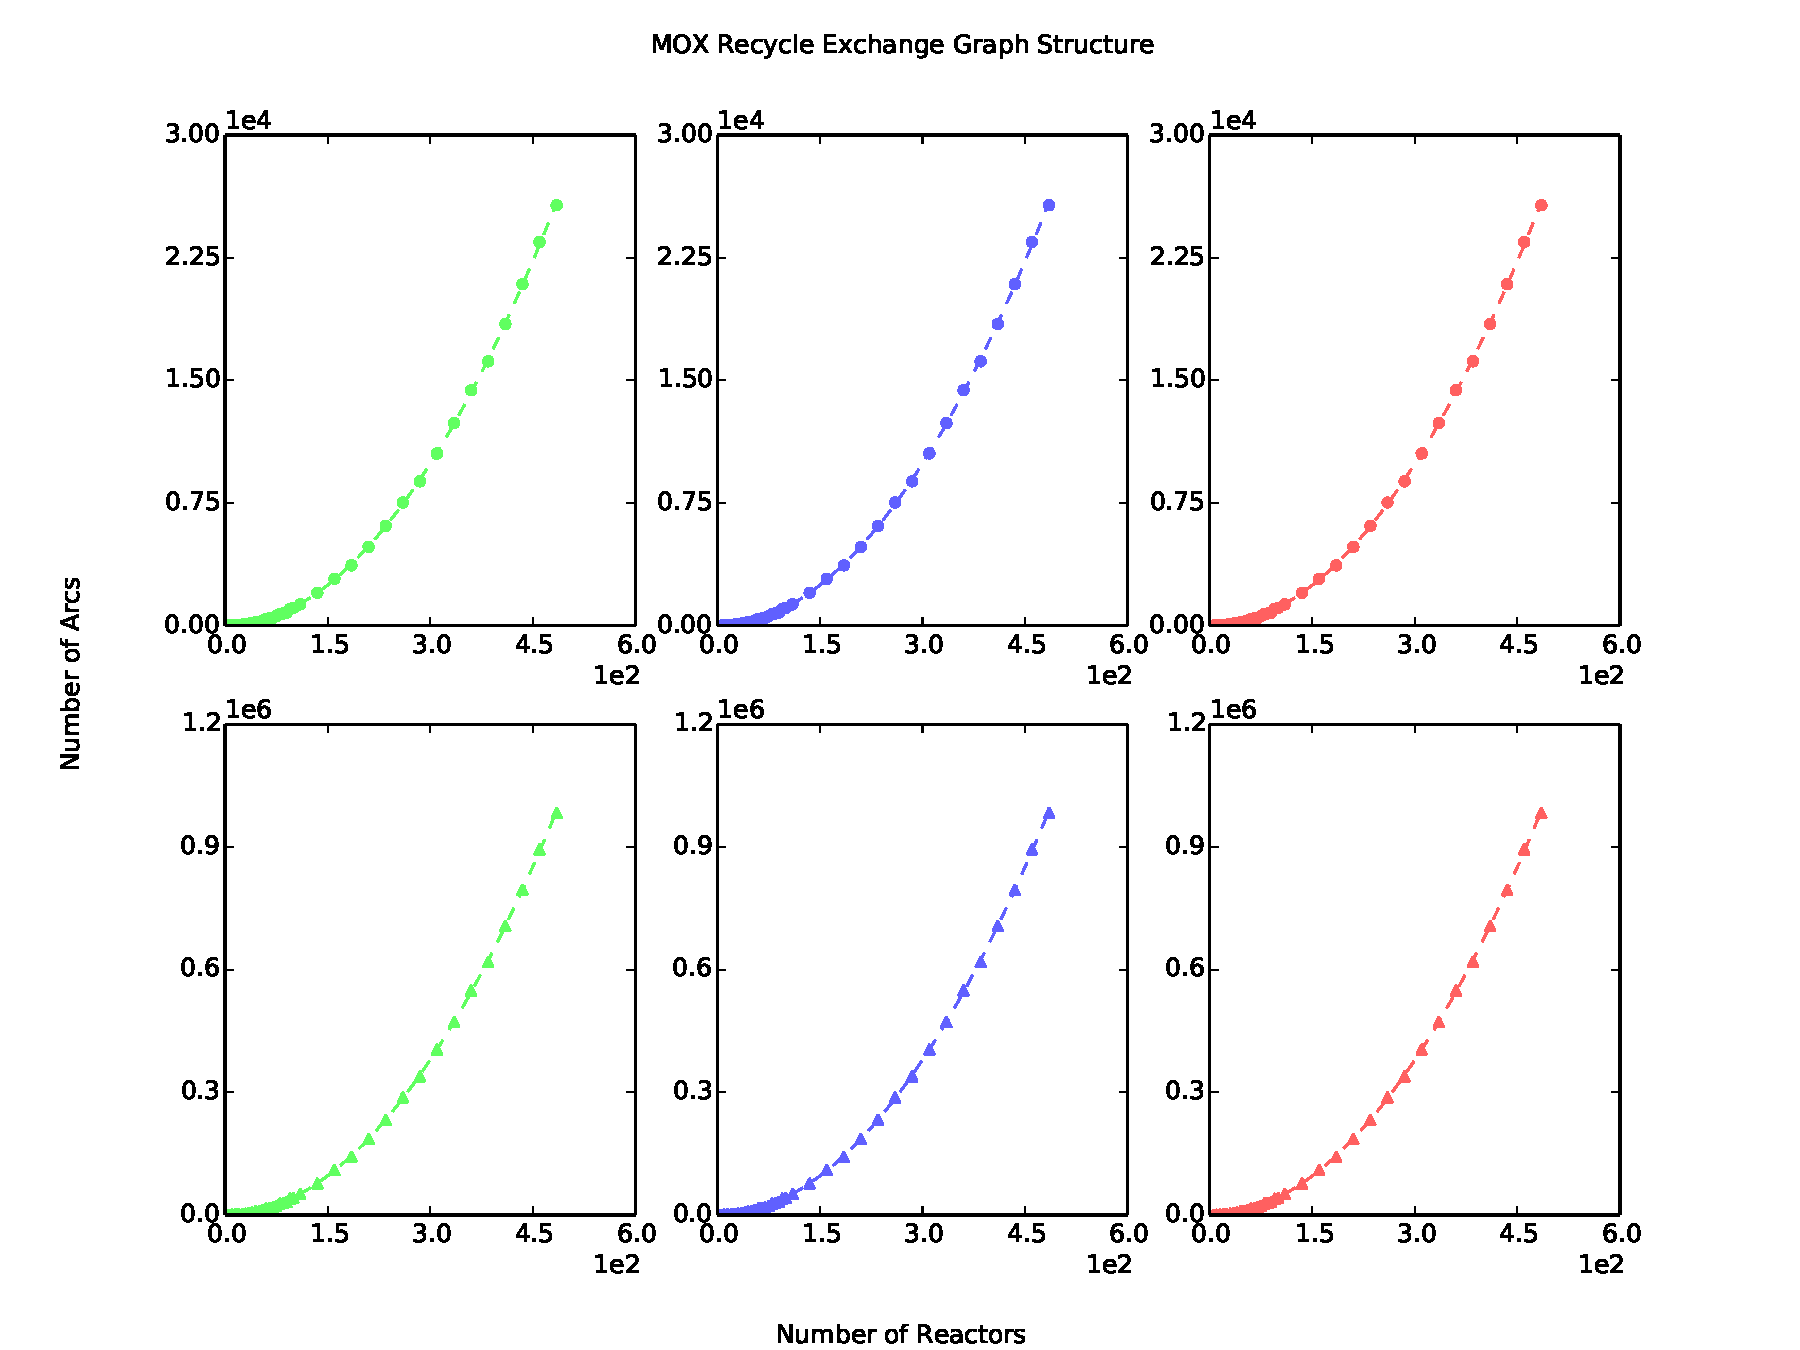
\includegraphics[width=.7\textwidth]{base_front_n_rxtr_n_arcs_fc1_solvergreedy.pdf}
    \caption[]{
      \label{fig:base_front_n_rxtr_n_arcs_fc1_solvergreedy}
      Arc population scaling with the number of reactors with coresponding linear fits.}
  \end{center}
\end{figure}

\begin{figure}[h!]
  \begin{center}
    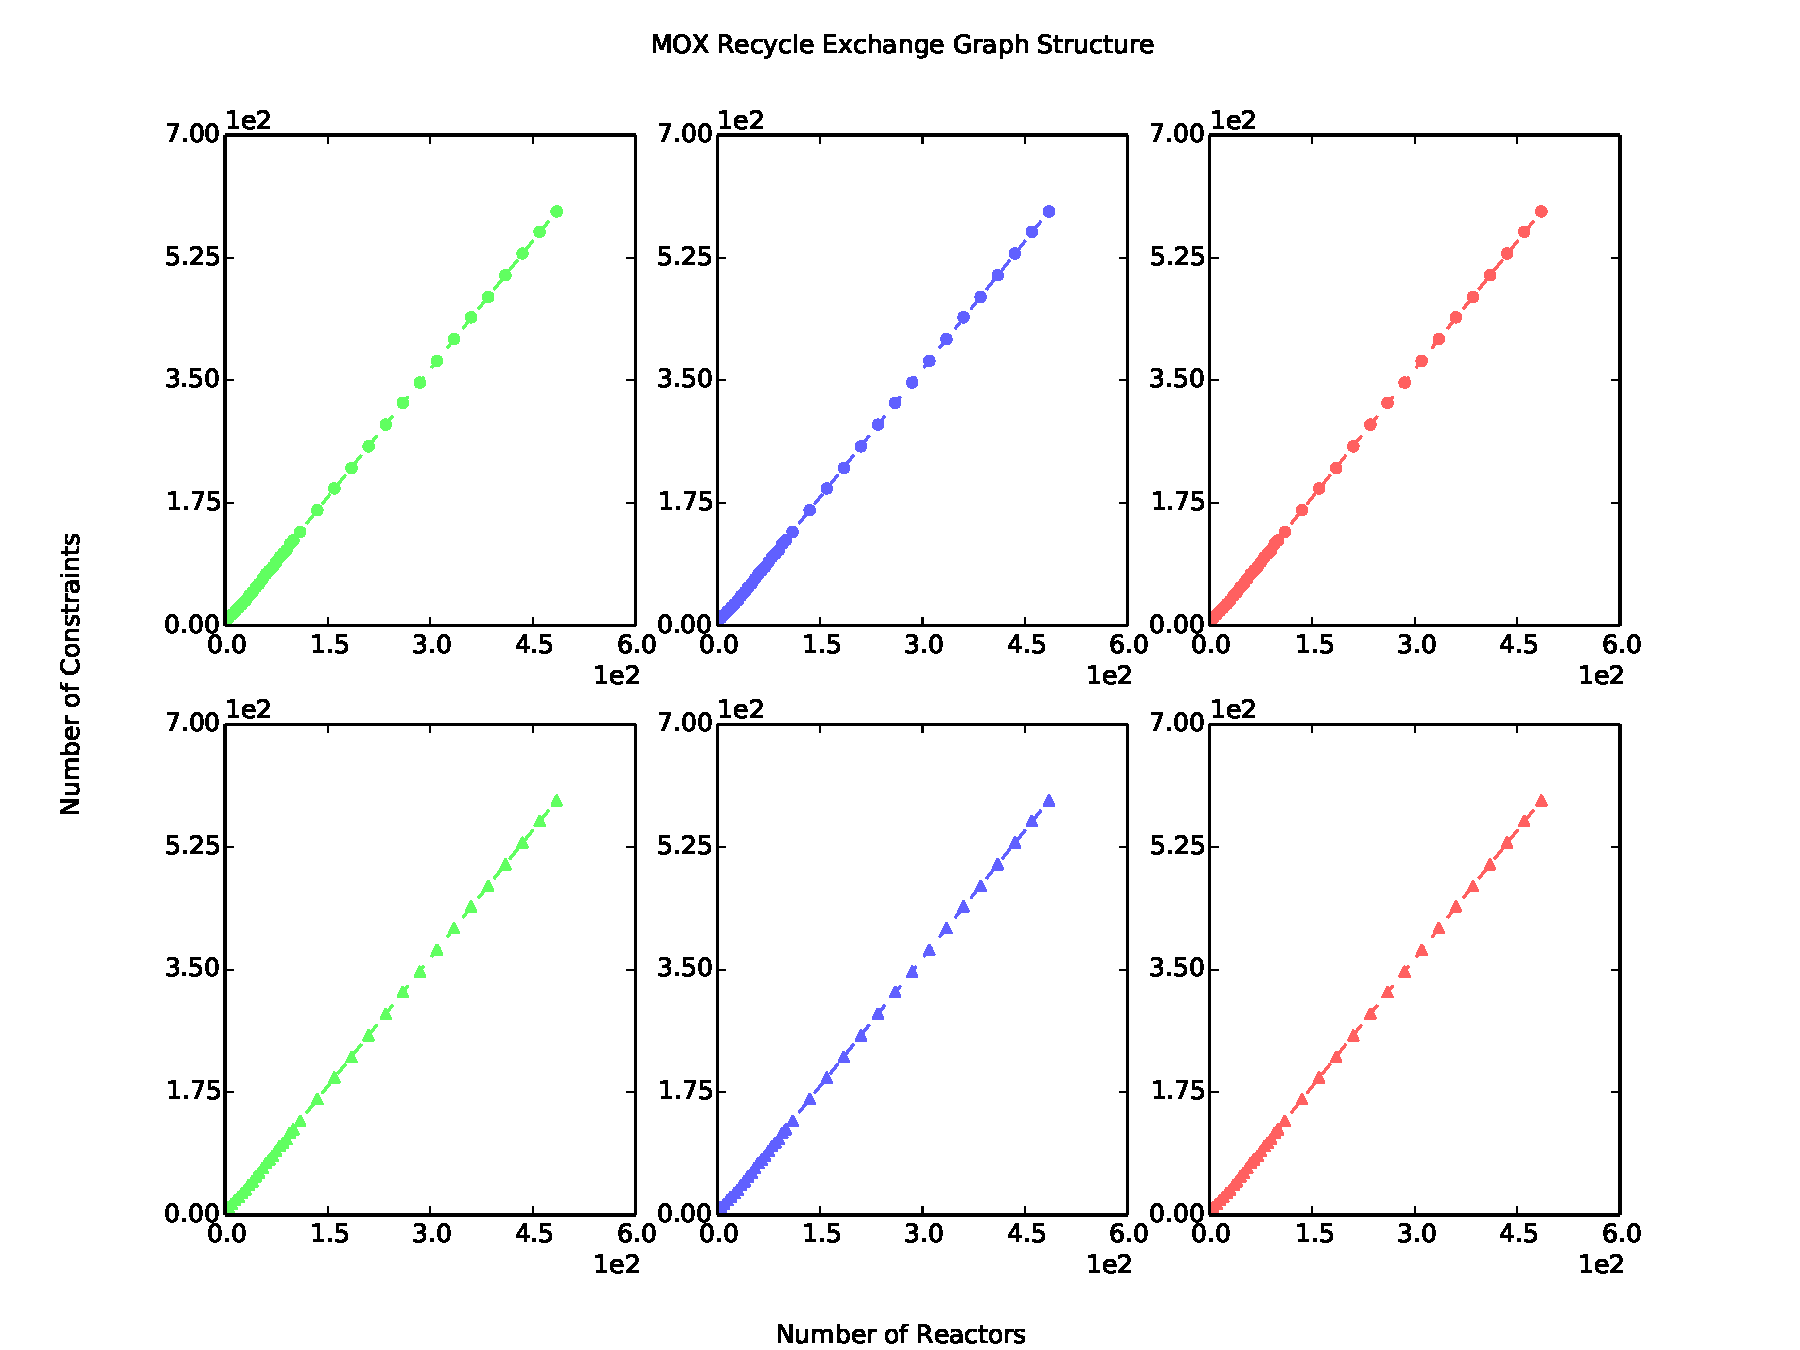
\includegraphics[width=.7\textwidth]{base_front_n_rxtr_n_constrs_fc1_solvergreedy.pdf}
    \caption[]{
      \label{fig:base_front_n_rxtr_n_constrs_fc1_solvergreedy}
      Constraint population scaling with the number of reactors with
      corresponding quadratic fits.}
  \end{center}
\end{figure}


\paragraph{Greedy Solver}

\cref{fig:base_front_n_rxtr_time_fc0_solvergreedy,fig:base_front_n_rxtr_time_fc1_solvergreedy,fig:base_front_n_rxtr_time_fc2_solvergreedy}
show the Greedy Solver results as the number of reactors increases for the OT,
MOX, and ThOX fuel cycles, respectively. Plotted with each data series is a
second-order polynomial fit, suggesting that the Greedy Solver scales as
$\mathcal{O}(n^2)$ in the number of reactors. As can be seen, this scaling is
independent of any fundamental parameter, as it is seen in every combination
thereof.

\begin{figure}[h!]
  \begin{center}
    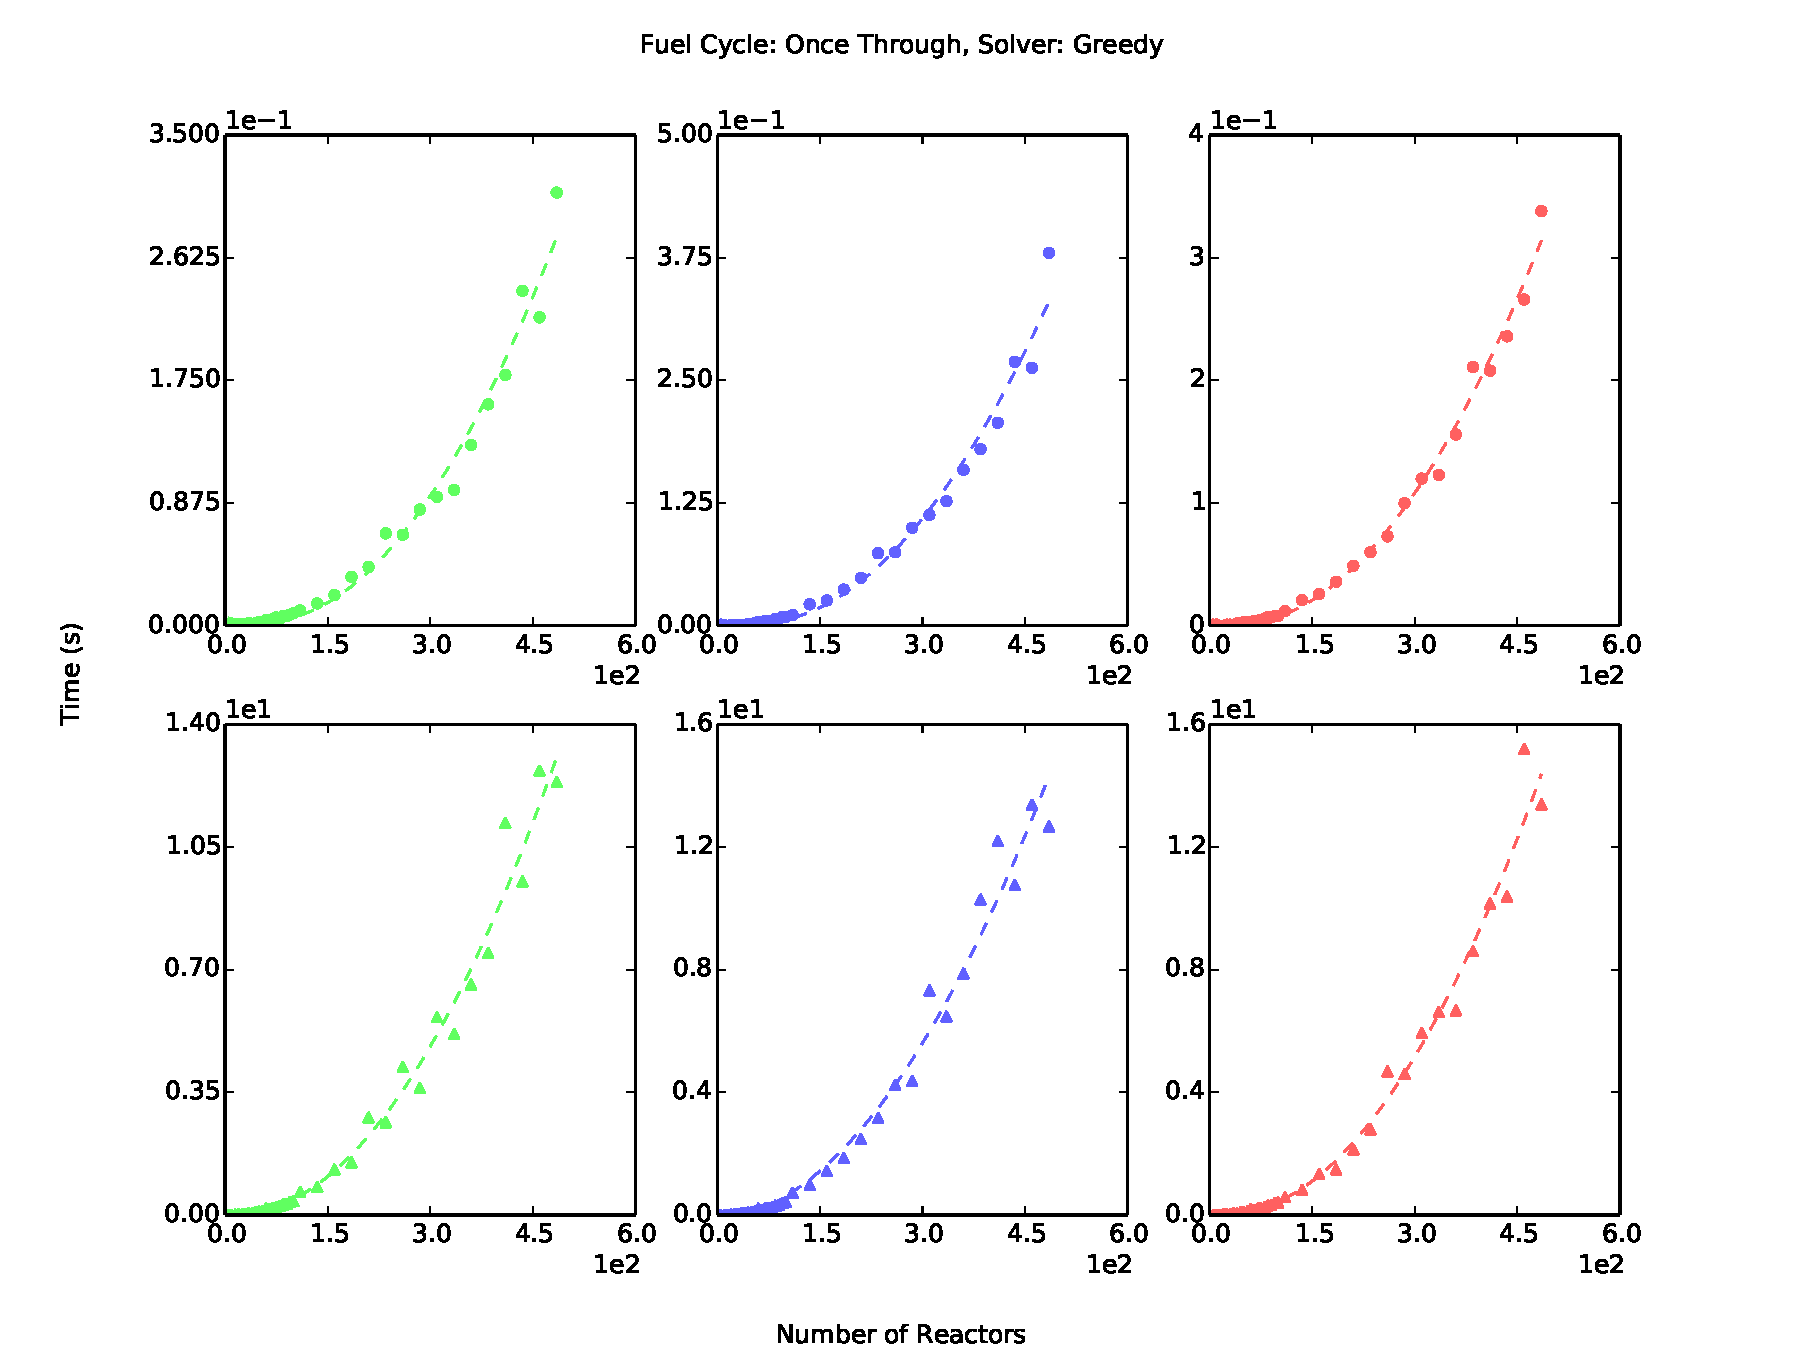
\includegraphics[width=.7\textwidth]{base_front_n_rxtr_time_fc0_solvergreedy.pdf}
    \caption[]{
      \label{fig:base_front_n_rxtr_time_fc0_solvergreedy}
      Greedy Solver results for the OT fuel cycle as the number of reactors
      increases.  }
  \end{center}
\end{figure}

\begin{figure}[h!]
  \begin{center}
    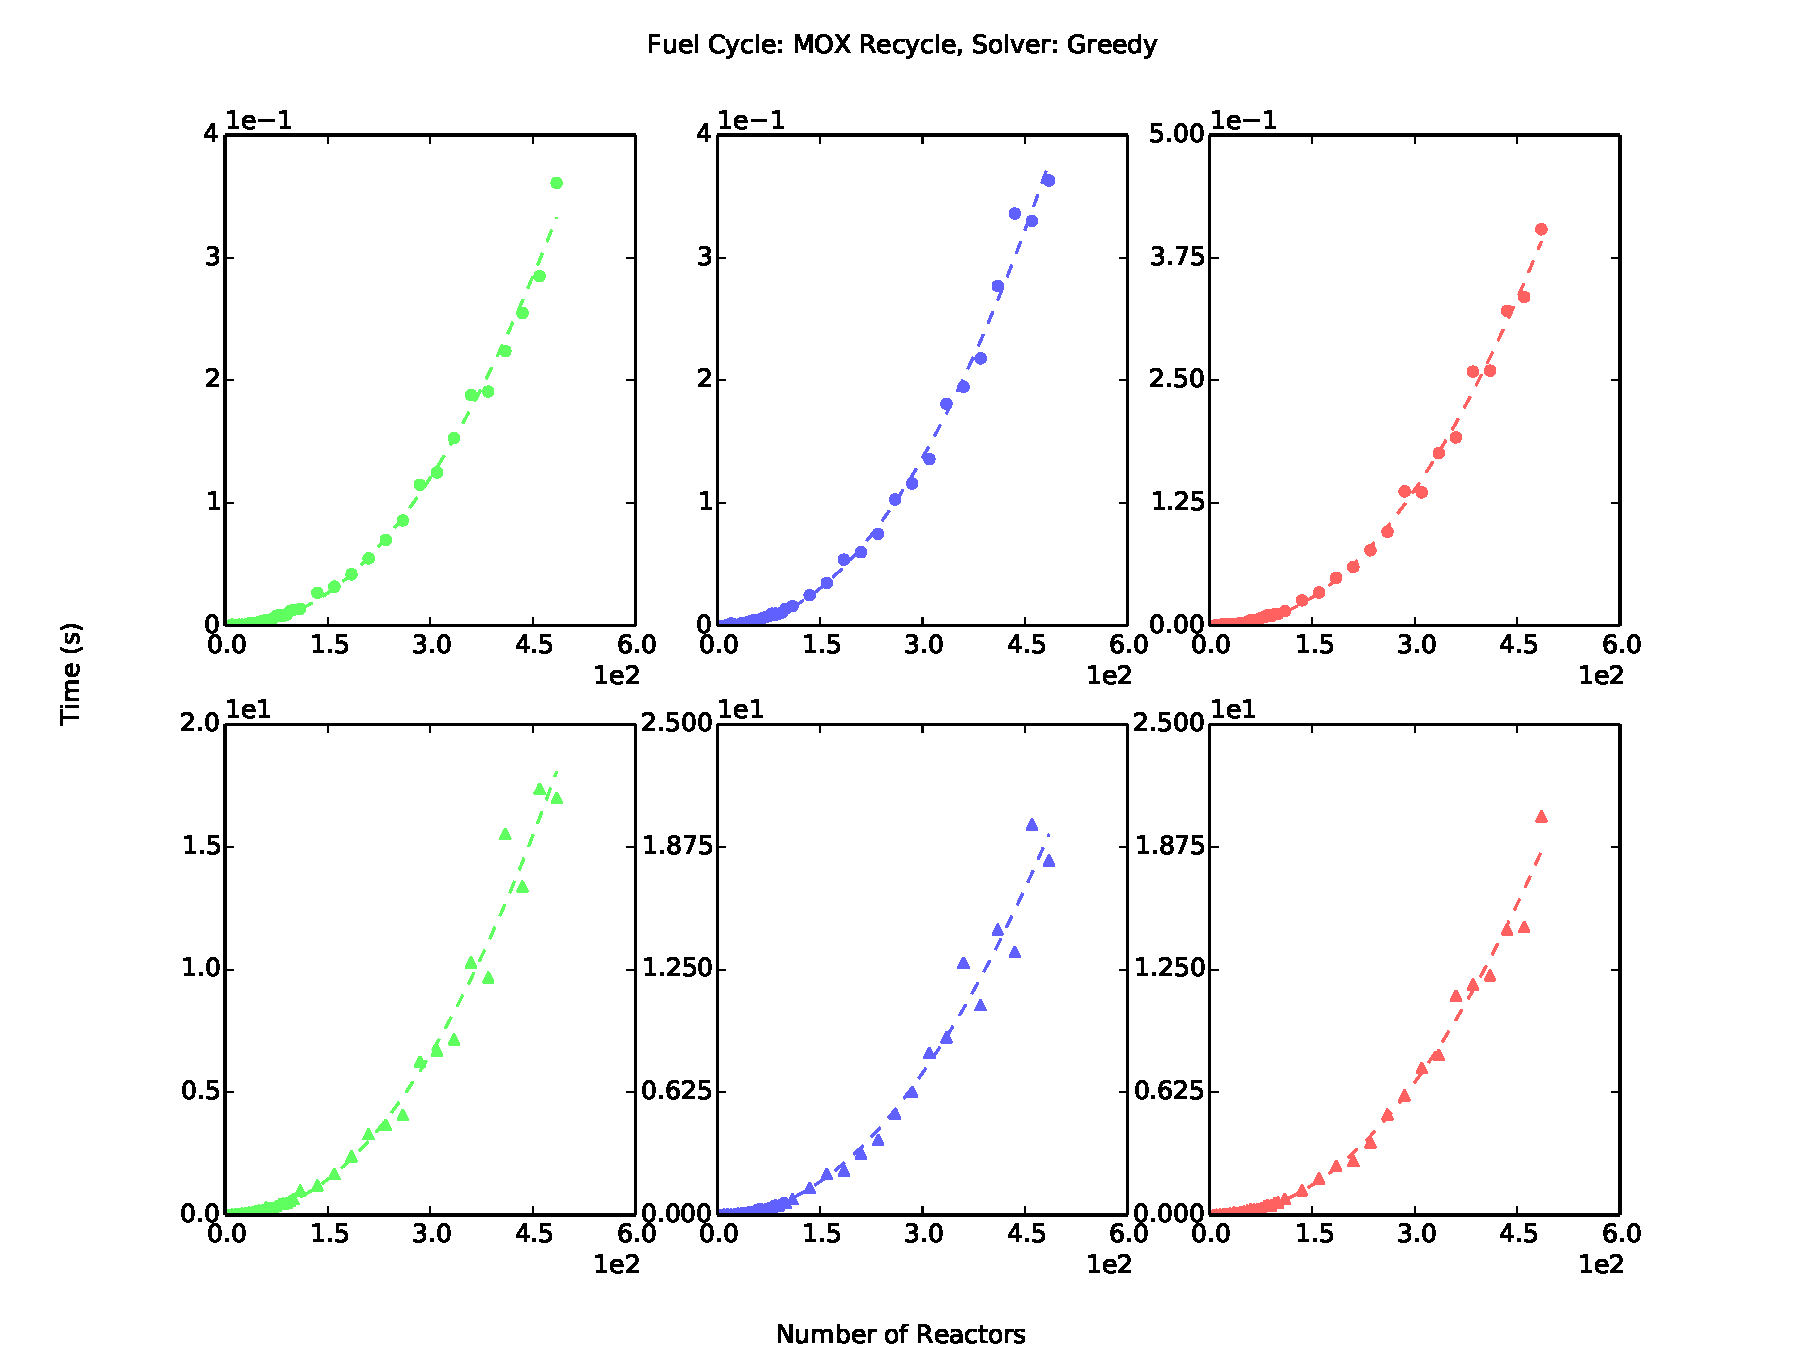
\includegraphics[width=.7\textwidth]{base_front_n_rxtr_time_fc1_solvergreedy.pdf}
    \caption[]{
      \label{fig:base_front_n_rxtr_time_fc1_solvergreedy}
      Greedy Solver results for the MOX fuel cycle as the number of reactors
      increases.
    }
  \end{center}
\end{figure}

\begin{figure}[h!]
  \begin{center}
    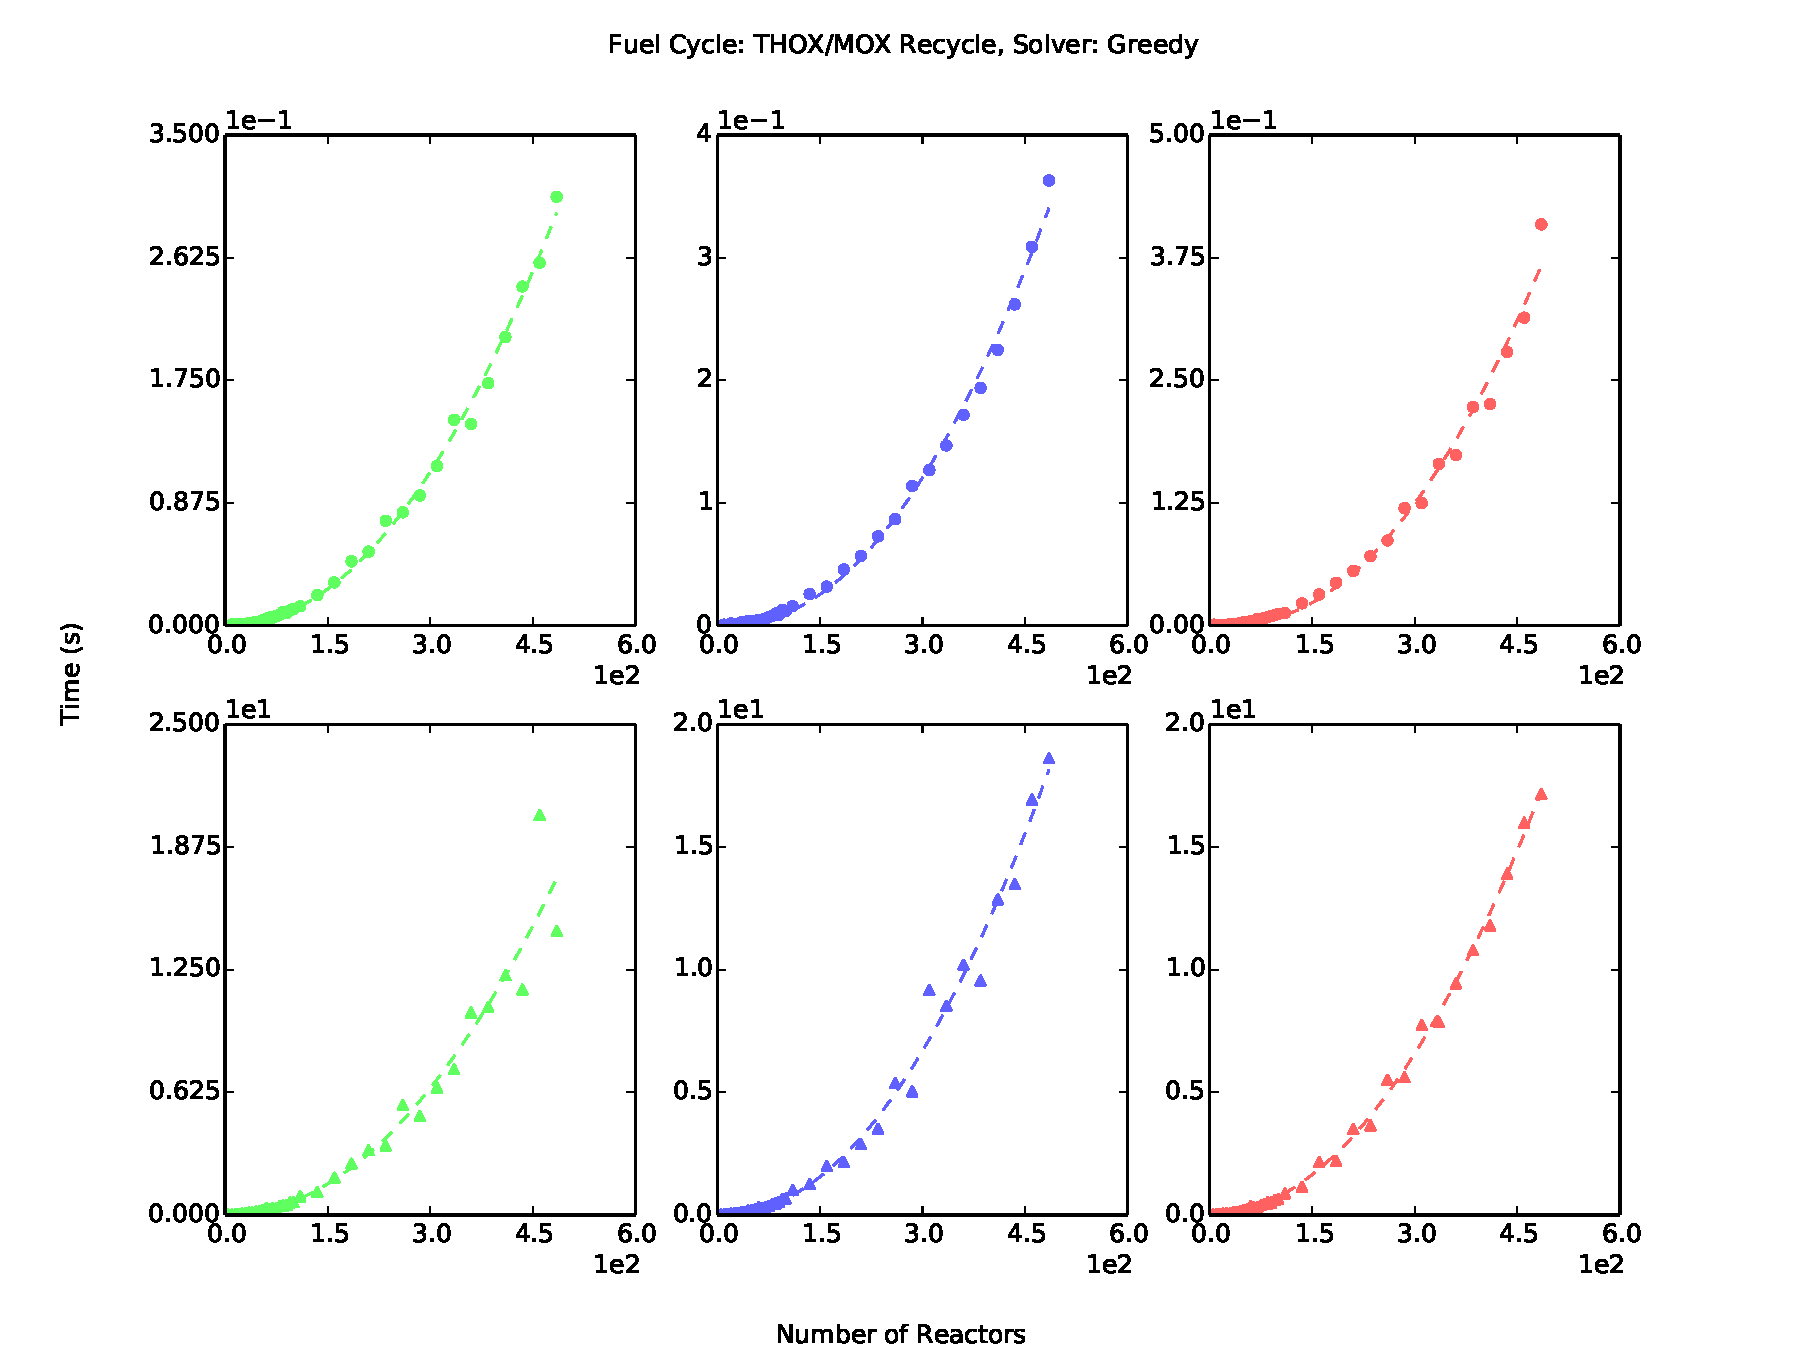
\includegraphics[width=.7\textwidth]{base_front_n_rxtr_time_fc2_solvergreedy.pdf}
    \caption[]{
      \label{fig:base_front_n_rxtr_time_fc2_solvergreedy}
      Greedy Solver results for the ThOX fuel cycle as the number of reactors
      increases.
      }
  \end{center}
\end{figure}

As was shown previously, the number of arcs in a generated exchange is an
$\mathcal{O}(n^2)$ effect. \ref{fig:base_front_n_arcs_time_fc1_solvergreedy}
graphs the same solution populations shown previously for the MOX fuel cycle as
a function of the number of arcs in the system. Plotted alongside the data are
linear curve fits. As can be seen, solution times scale linearly with the number
of arcs in the system. These trends are consistent across all three modeled fuel
cycles.

\begin{figure}[h!]
  \begin{center}
    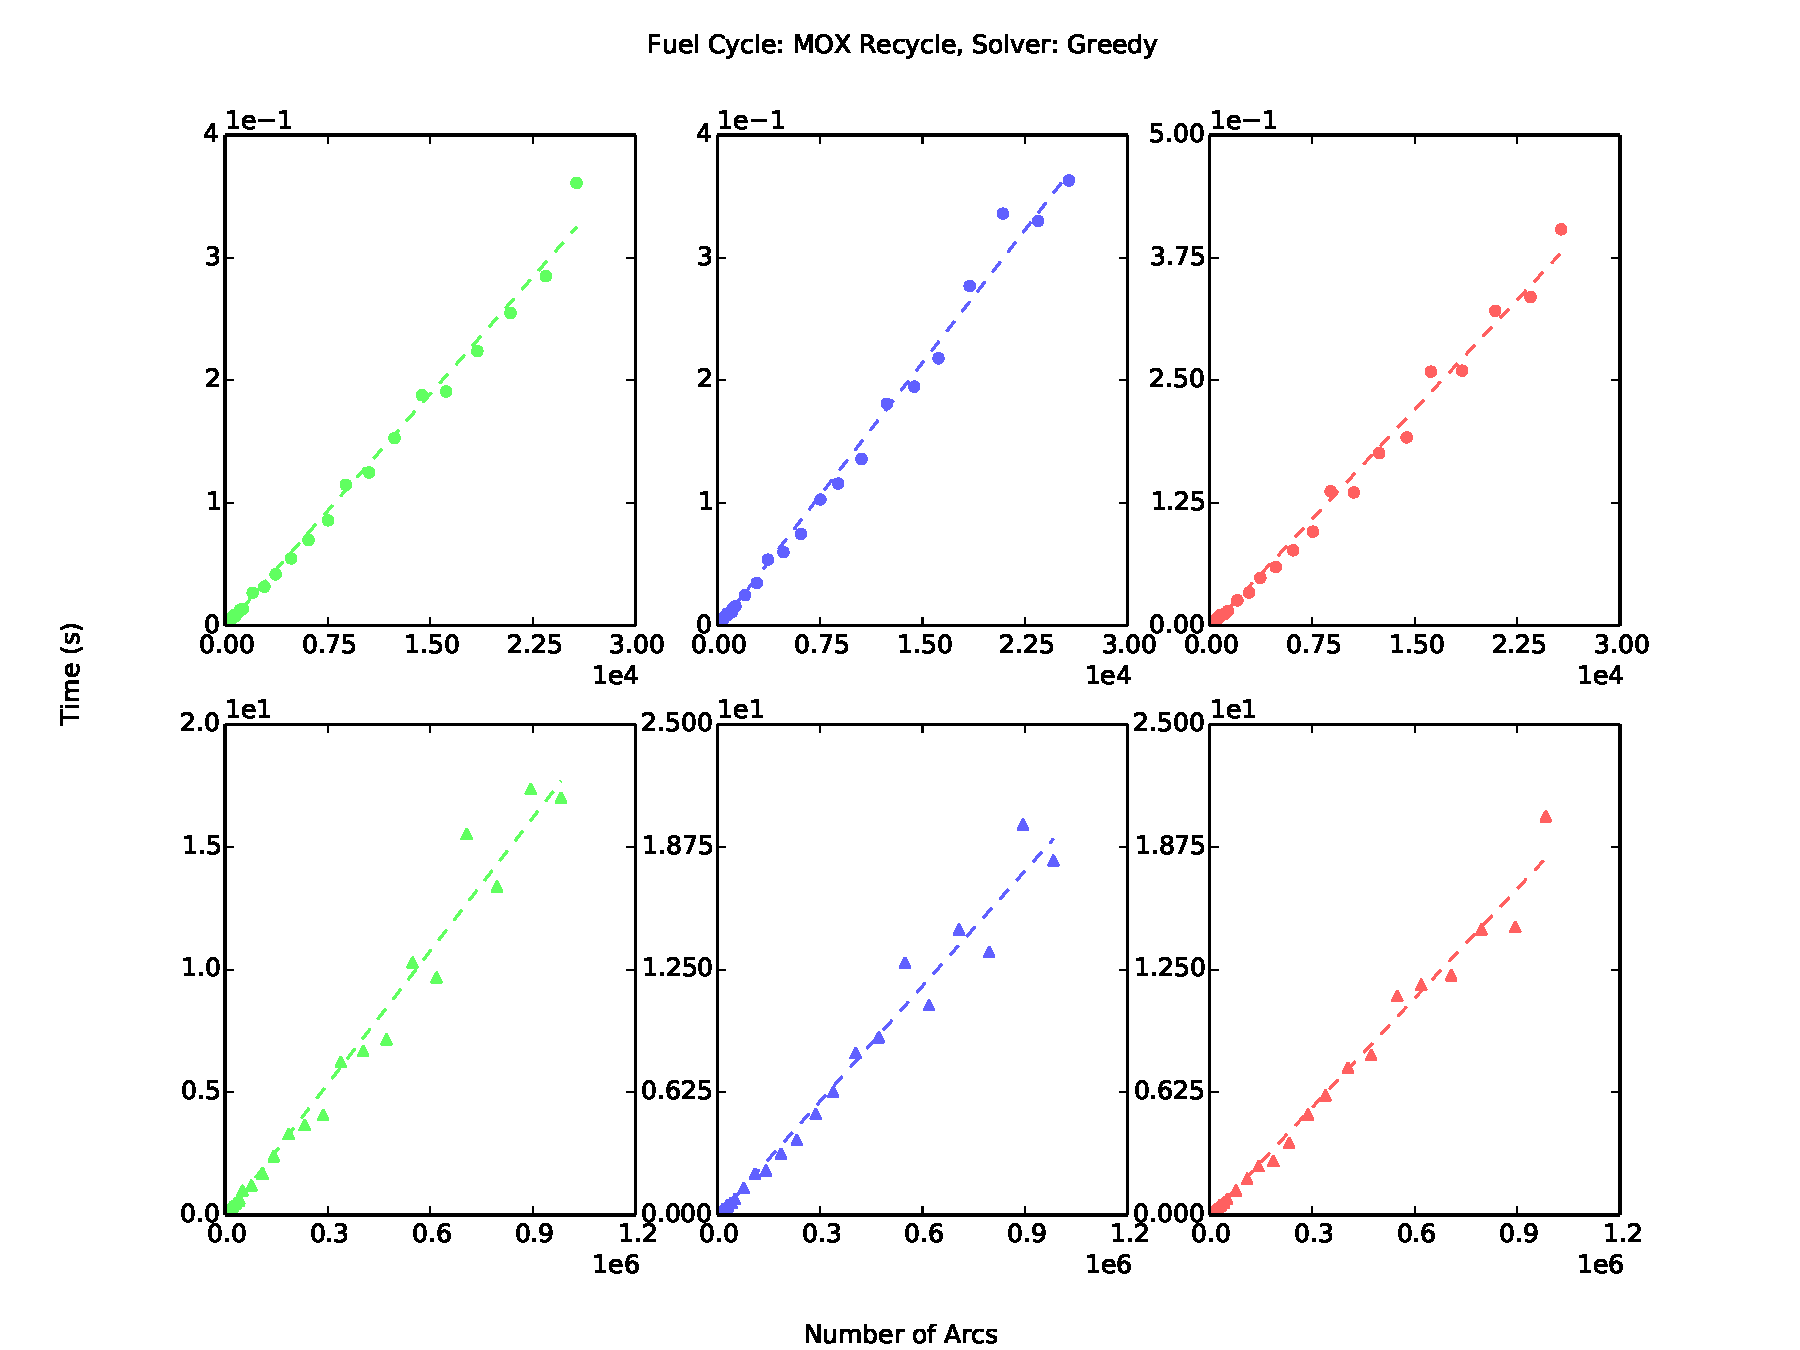
\includegraphics[width=.7\textwidth]{base_front_n_arcs_time_fc1_solvergreedy.pdf}
    \caption[]{
      \label{fig:base_front_n_arcs_time_fc1_solvergreedy}
      Greedy Solver results for the MOX fuel cycle as the number of arcs
      increases.      
    }
  \end{center}
\end{figure}

\paragraph{CLP Solver}

Interestingly, the CLP solver shows the same scaling behavior as the Greedy
Solver, and that behavior is also independent of fundamental parameter. The
number of arcs in the system drives the solution time scaling, as can be seen in
\Cref{fig:base_front_n_arcs_time_fc0_solverclp,fig:base_front_n_arcs_time_fc1_solverclp,fig:base_front_n_arcs_time_fc2_solverclp}.

\begin{figure}[h!]
  \begin{center}
    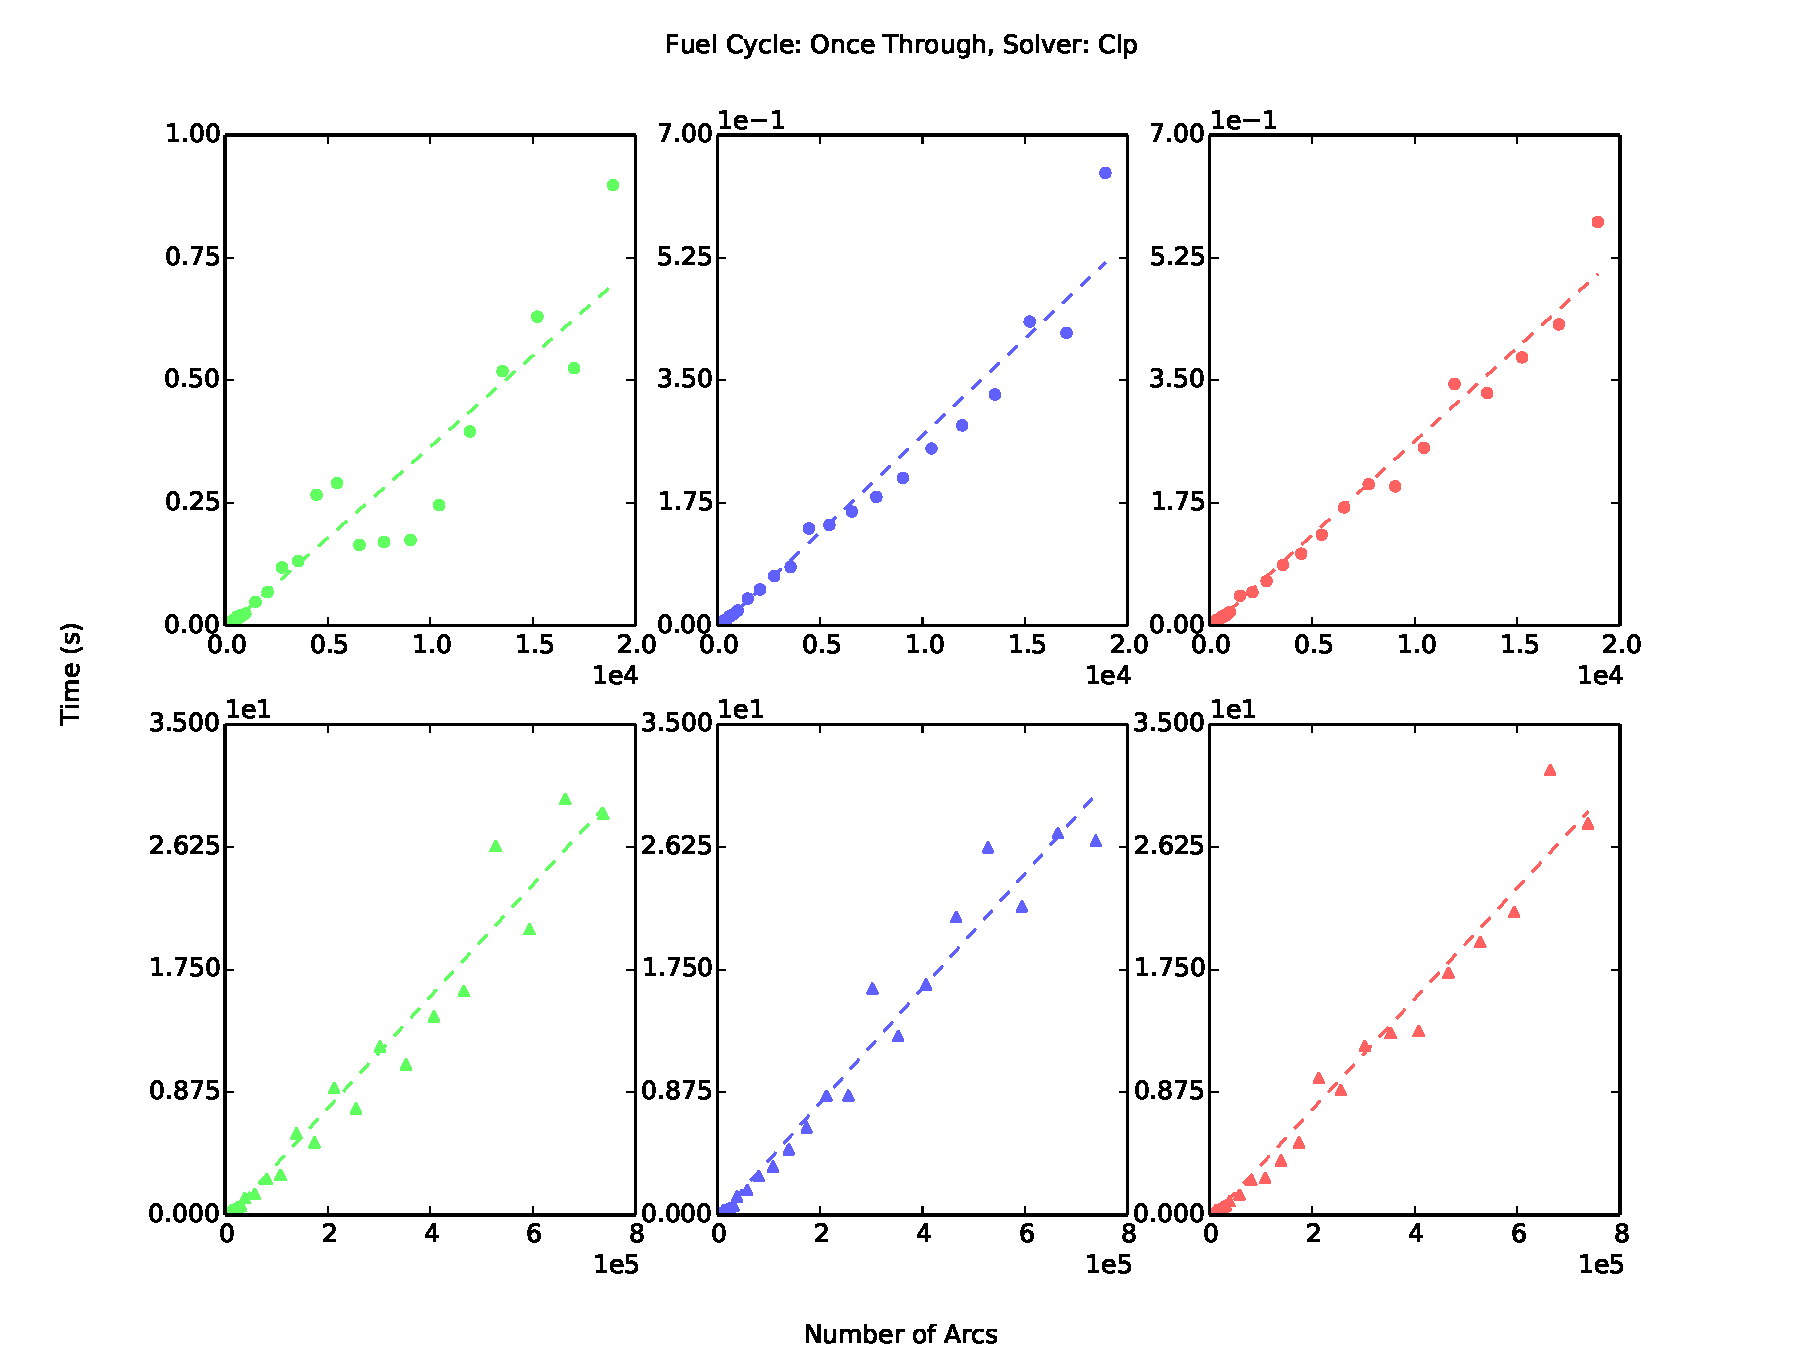
\includegraphics[width=.7\textwidth]{base_front_n_arcs_time_fc0_solverclp.pdf}
    \caption[]{
      \label{fig:base_front_n_arcs_time_fc0_solverclp}
      CLP Solver results for the OT fuel cycle as the number of arcs
      increases.
      }
  \end{center}
\end{figure}

\begin{figure}[h!]
  \begin{center}
    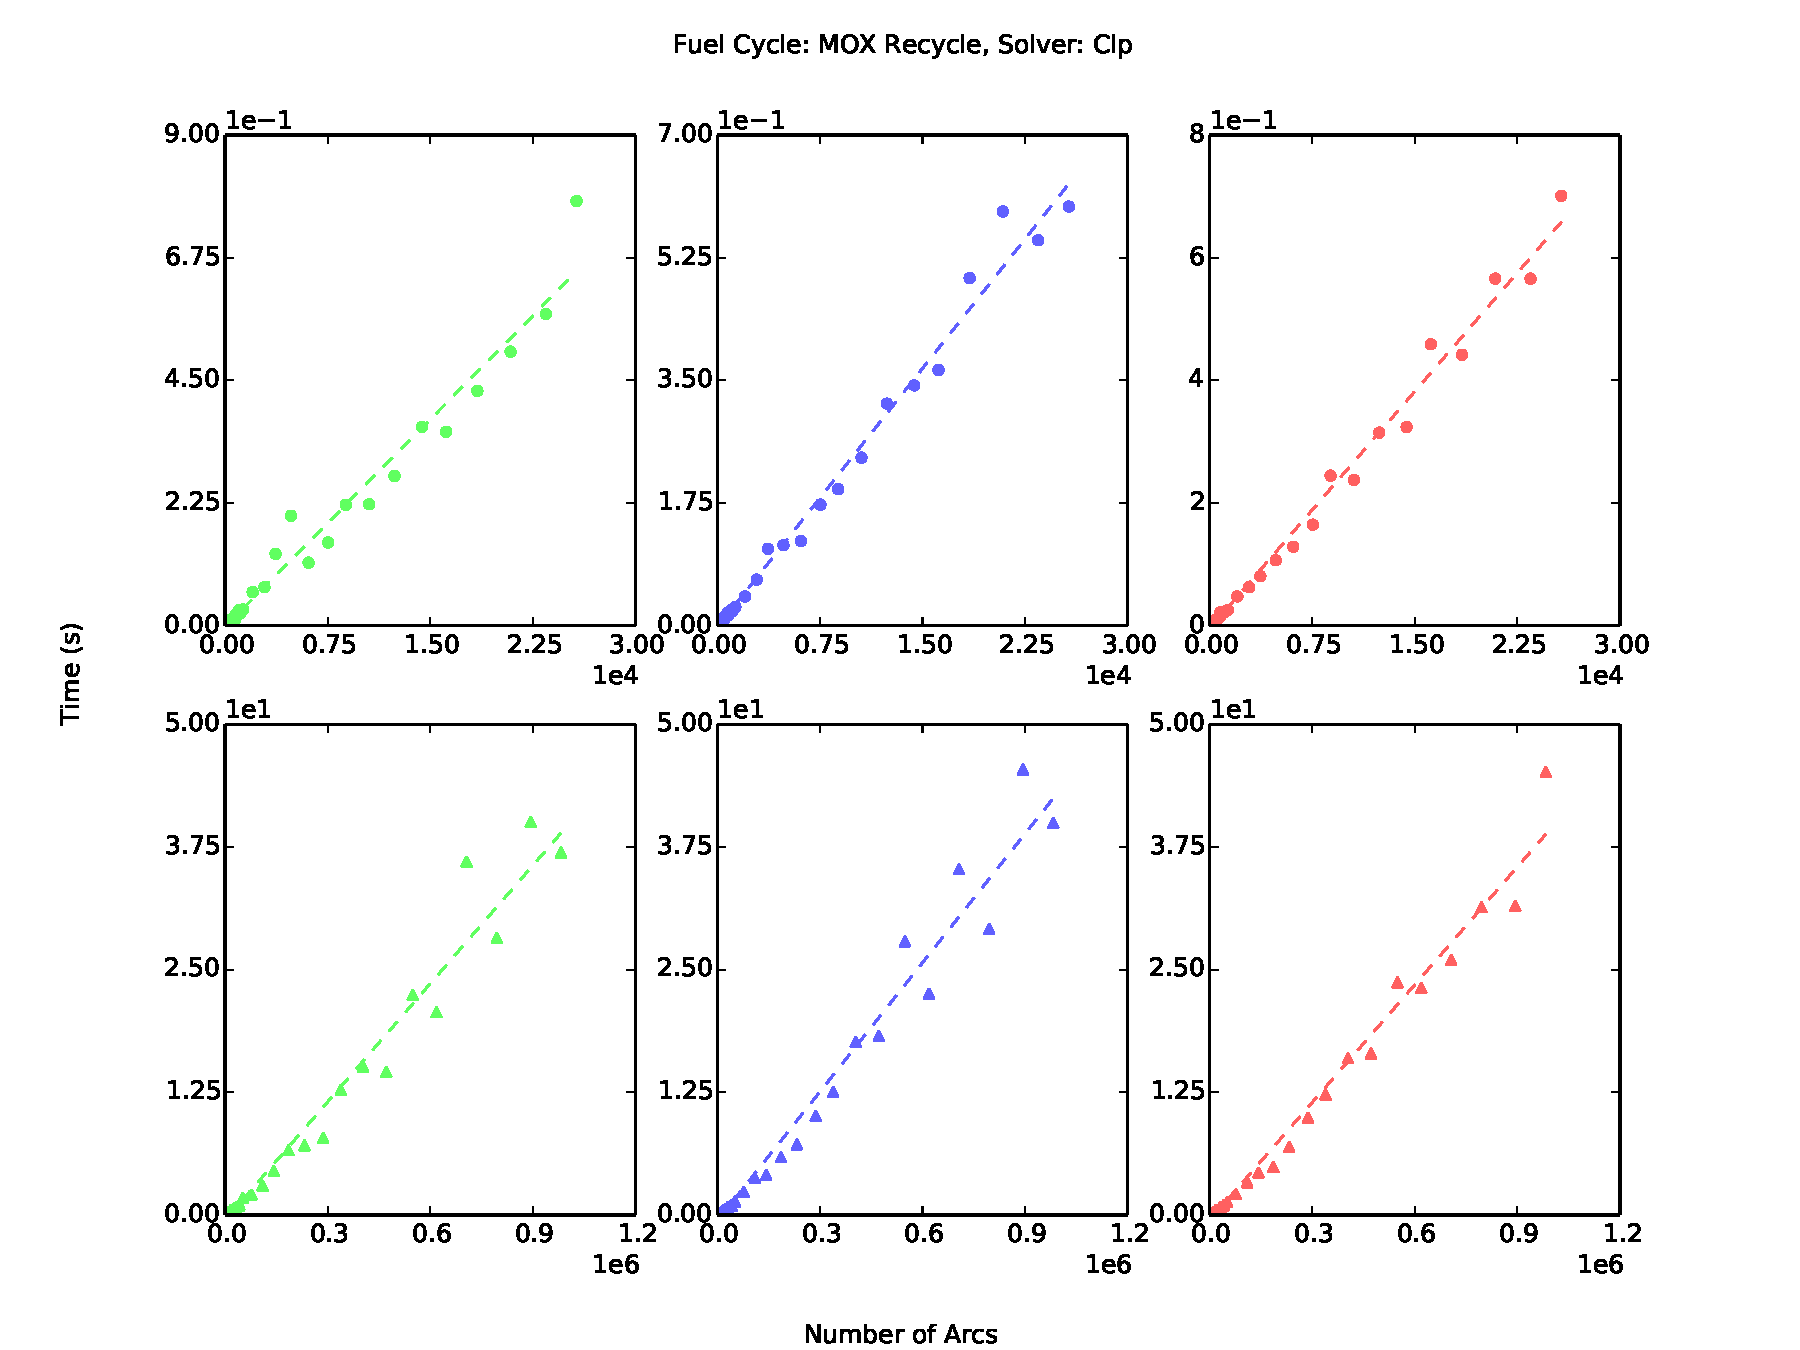
\includegraphics[width=.7\textwidth]{base_front_n_arcs_time_fc1_solverclp.pdf}
    \caption[]{
      \label{fig:base_front_n_arcs_time_fc1_solverclp}
      CLP Solver results for the MOX fuel cycle as the number of arcs
      increases.
      }
  \end{center}
\end{figure}

\begin{figure}[h!]
  \begin{center}
    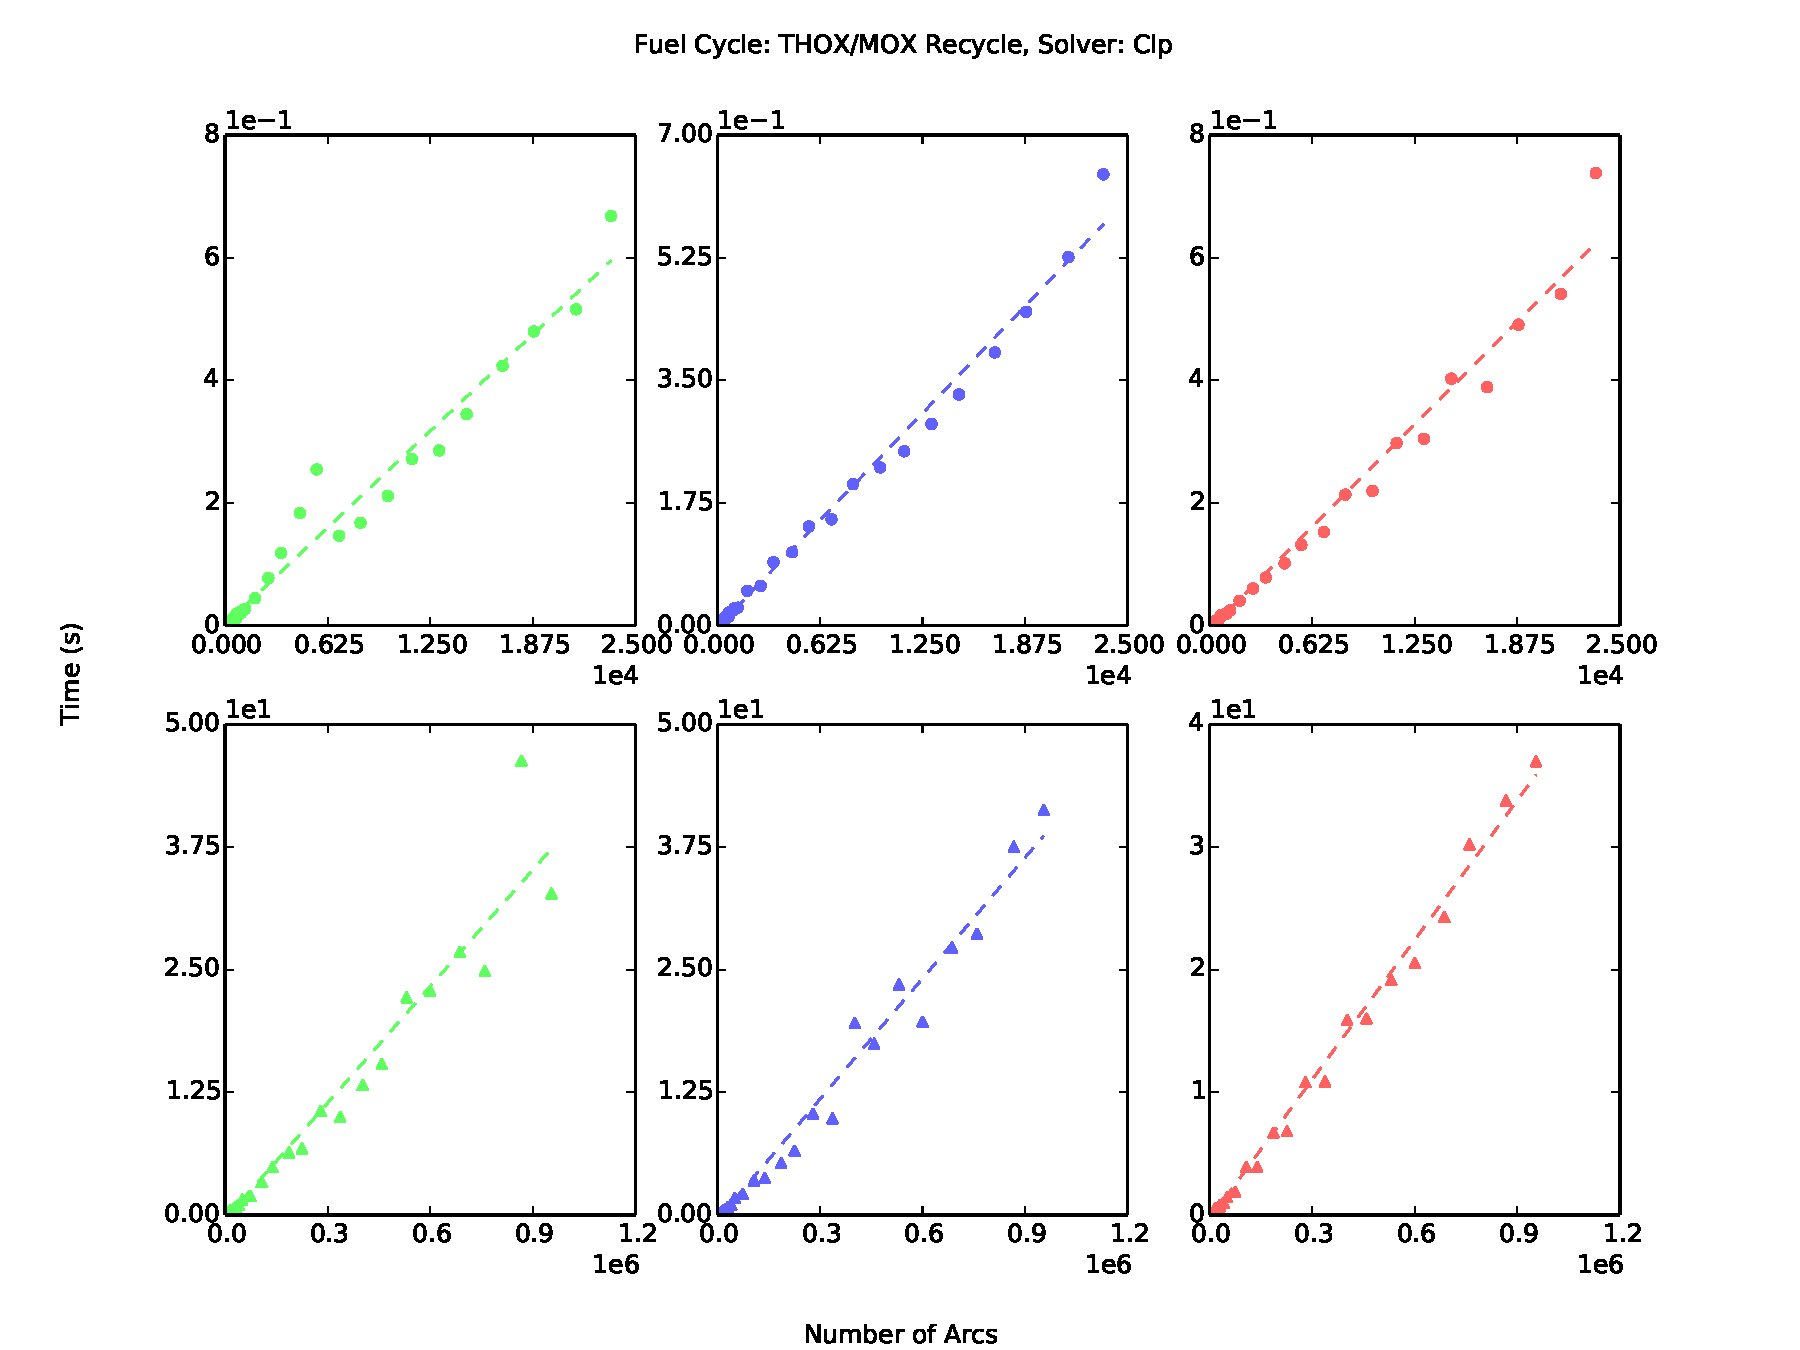
\includegraphics[width=.7\textwidth]{base_front_n_arcs_time_fc2_solverclp.pdf}
    \caption[]{
      \label{fig:base_front_n_arcs_time_fc2_solverclp}
      CLP Solver results for the ThOX fuel cycle as the number of arcs
      increases.
      }
  \end{center}
\end{figure}

\paragraph{CBC Solver}

The CBC solver is much more sporadic than either the CLP or Greedy solvers, as
is expected, for MILP optimization problems are NP-Hard. An artificial, 3-hour
time limit was provided for CBC-solved instances, and a 1\% ratio-gap
convergence criteria was applied. In each of the figures below, only instances
reaching convergence are displayed in order to attempt to ascertain any related
trends. \Cref{fig:base_front_n_rxtr_time_fc0_solvercbc,fig:base_front_n_rxtr_time_fc1_solvercbc,fig:base_front_n_rxtr_time_fc2_solvercbc}
show timing results as a function of the number of reactors in the
system. \Cref{fig:base_front_n_arcs_time_fc0_solvercbc,fig:base_front_n_arcs_time_fc1_solvercbc,fig:base_front_n_arcs_time_fc2_solvercbc}
show timing results as a function of the number of arcs in the system. Note that
in each case below, a log-lin graph is used.

\begin{figure}[h!]
  \begin{center}
    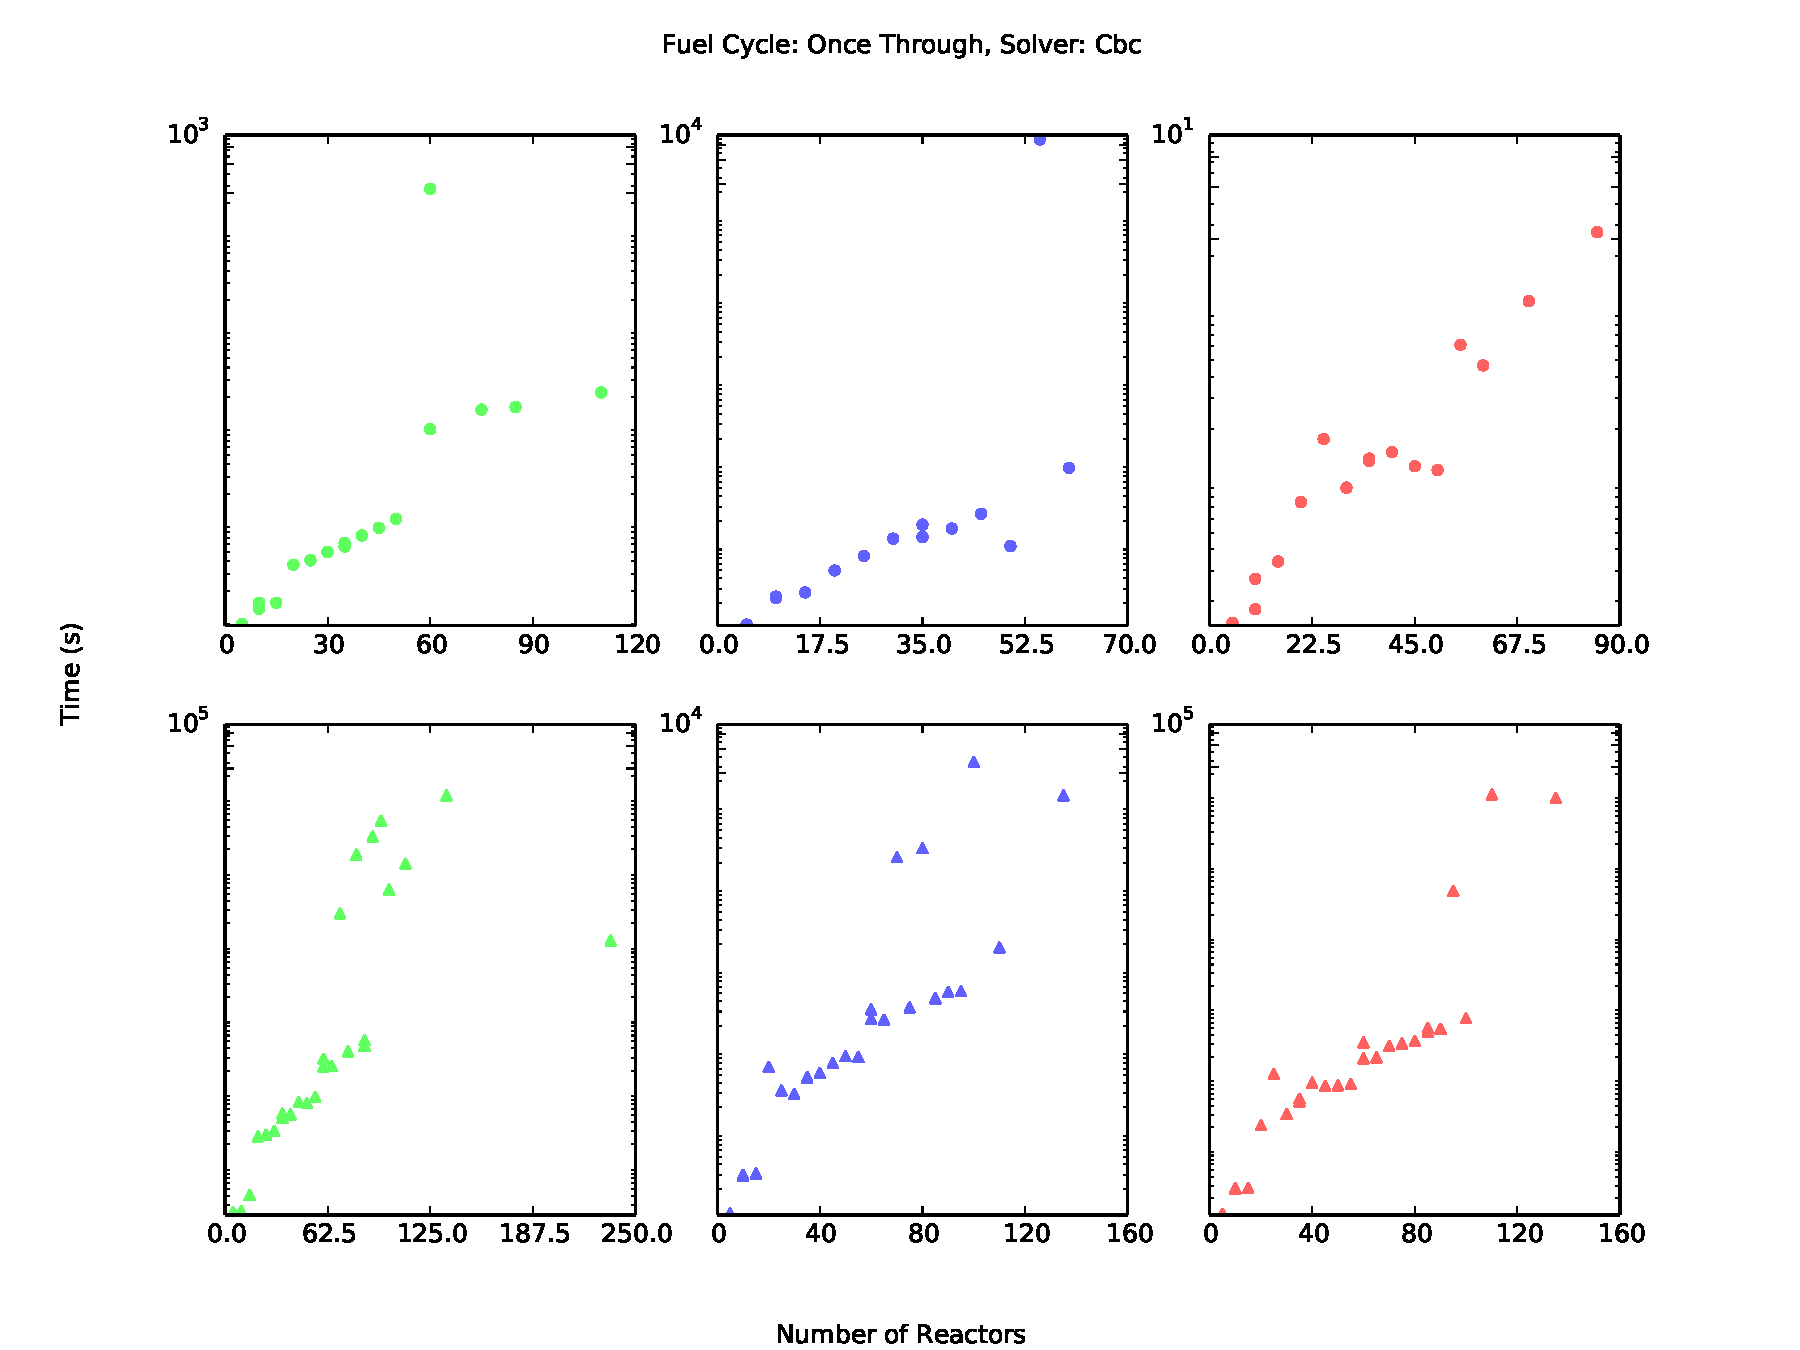
\includegraphics[width=.7\textwidth]{base_front_n_rxtr_time_fc0_solvercbc.pdf}
    \caption[]{
      \label{fig:base_front_n_rxtr_time_fc0_solvercbc}
      CBC Solver results for the OT fuel cycle as the number of reactors
      increases.
      }
  \end{center}
\end{figure}

\begin{figure}[h!]
  \begin{center}
    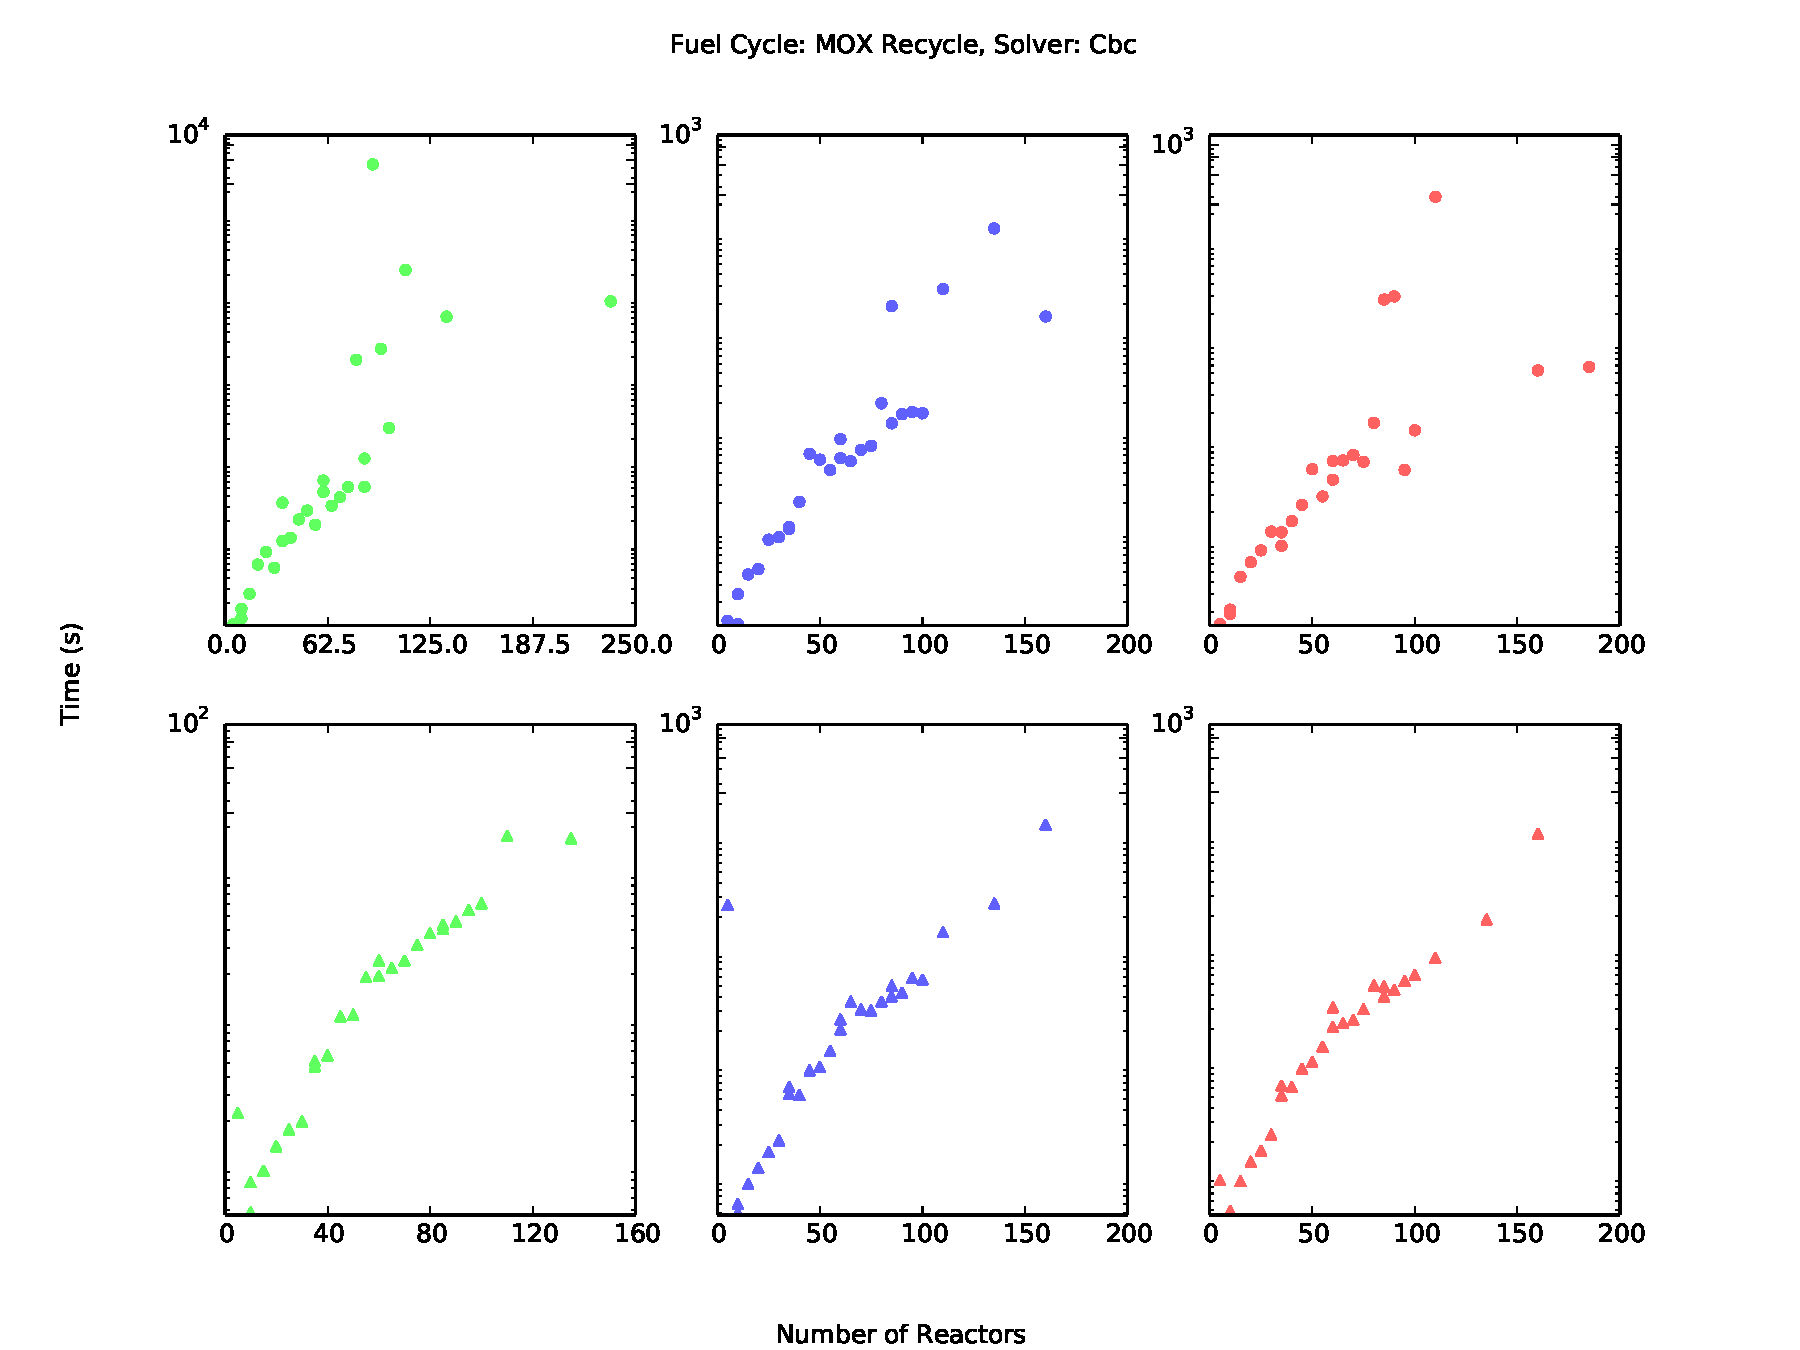
\includegraphics[width=.7\textwidth]{base_front_n_rxtr_time_fc1_solvercbc.pdf}
    \caption[]{
      \label{fig:base_front_n_rxtr_time_fc1_solvercbc}
      CBC Solver results for the MOX fuel cycle as the number of reactors
      increases.
      }
  \end{center}
\end{figure}

\begin{figure}[h!]
  \begin{center}
    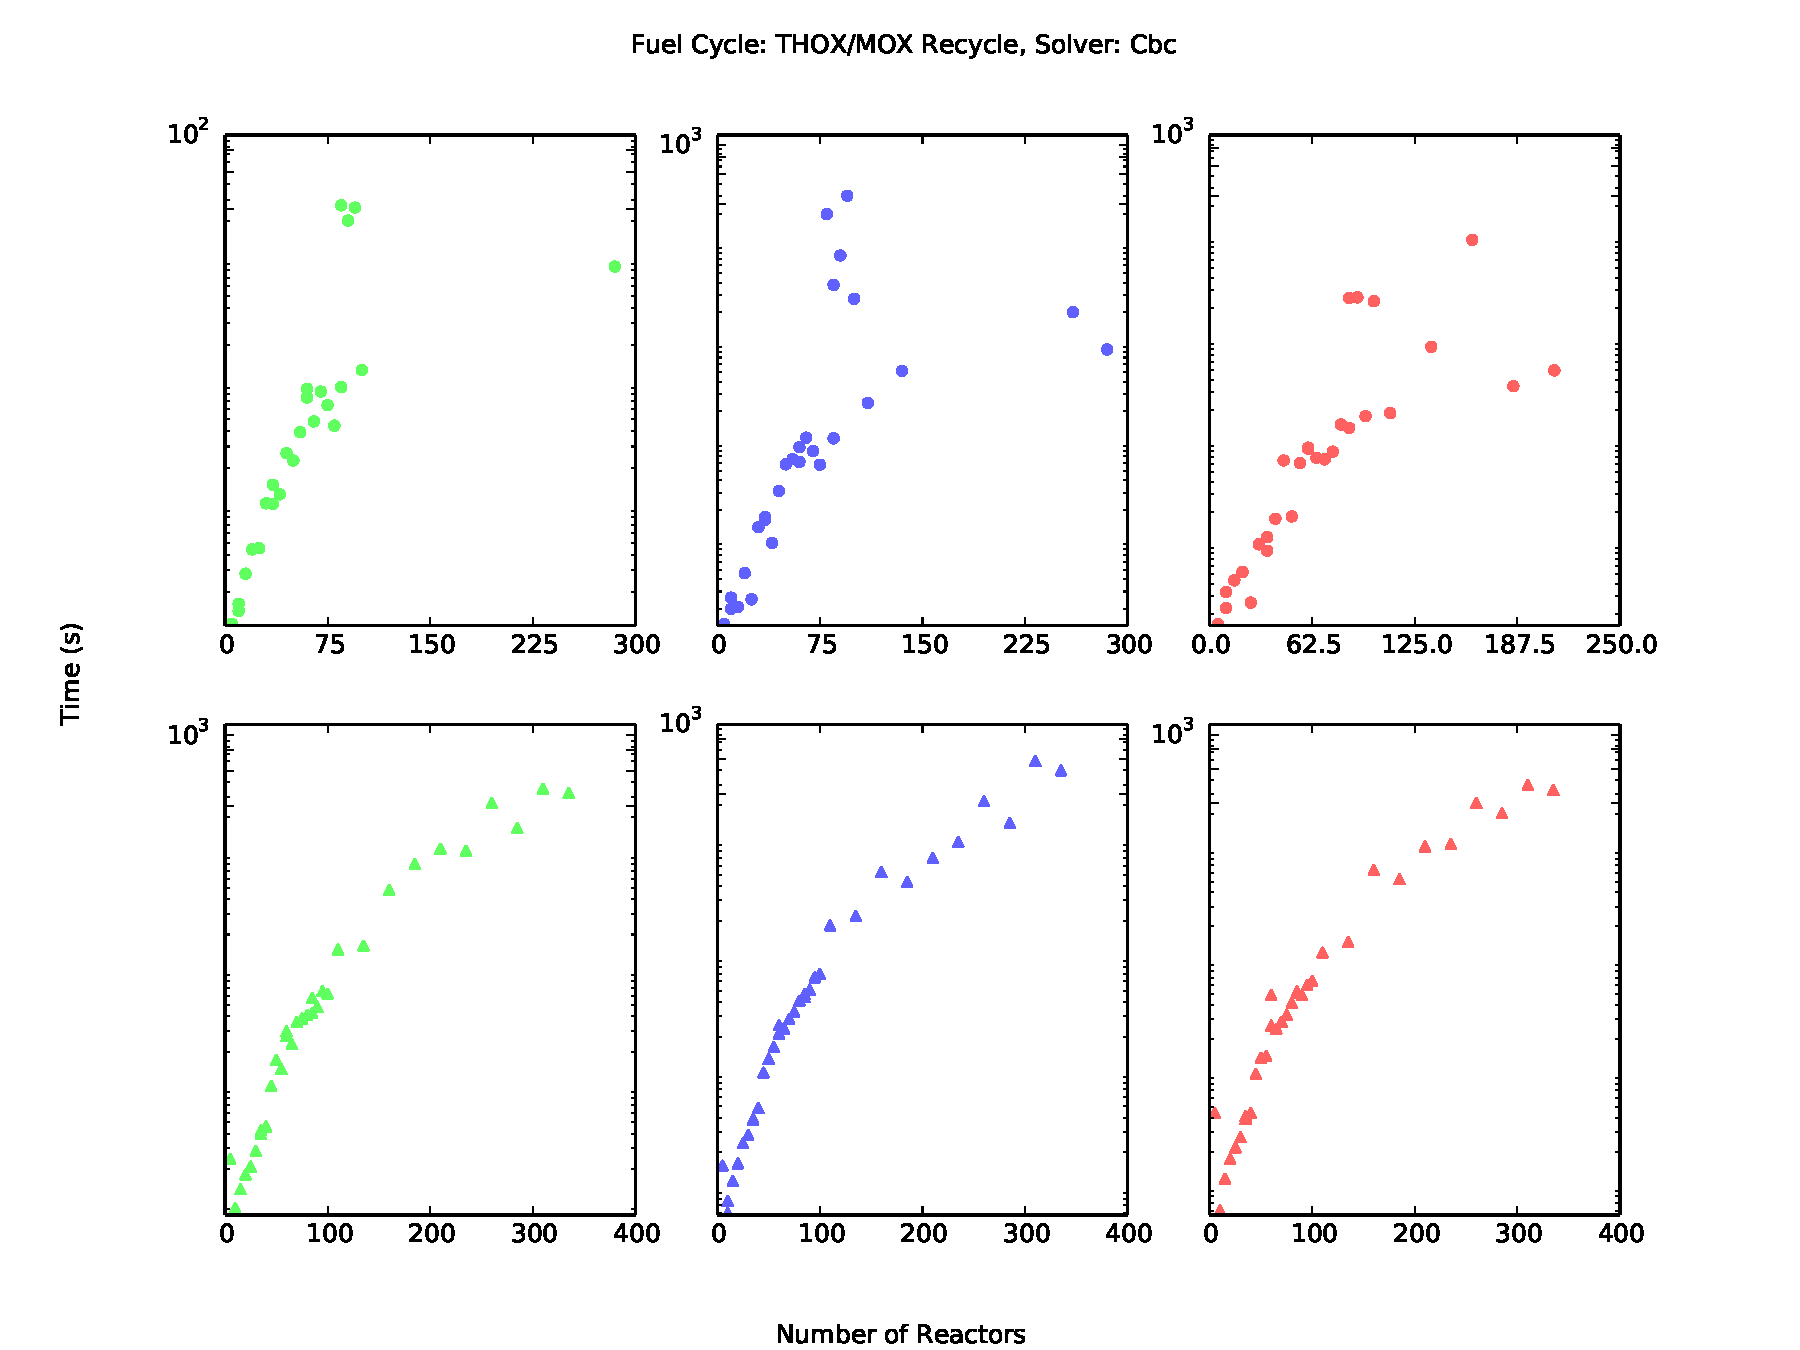
\includegraphics[width=.7\textwidth]{base_front_n_rxtr_time_fc2_solvercbc.pdf}
    \caption[]{
      \label{fig:base_front_n_rxtr_time_fc2_solvercbc}
      CBC Solver results for the ThOX fuel cycle as the number of reactors
      increases.
      }
  \end{center}
\end{figure}

\begin{figure}[h!]
  \begin{center}
    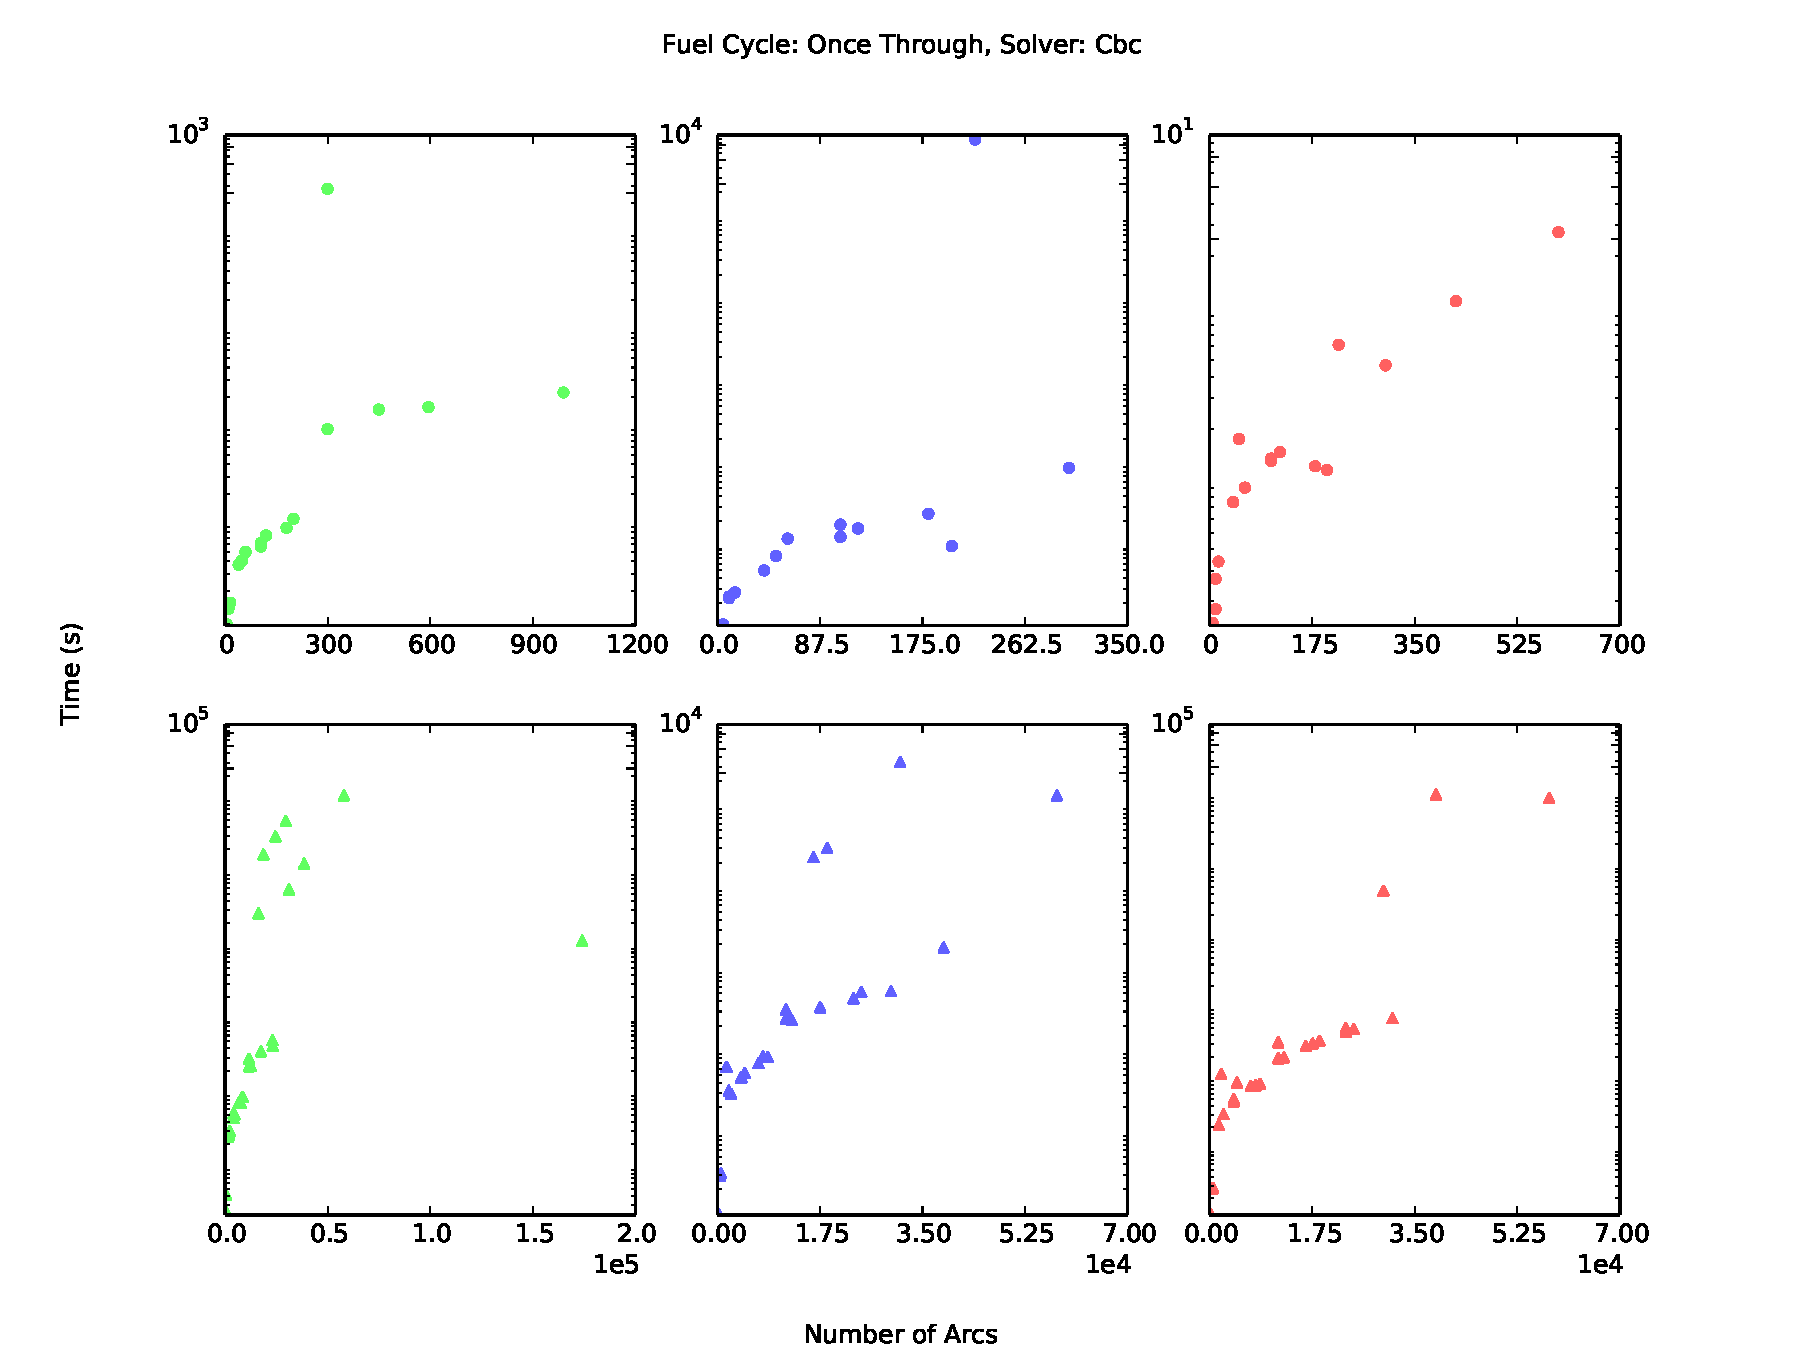
\includegraphics[width=.7\textwidth]{base_front_n_arcs_time_fc0_solvercbc.pdf}
    \caption[]{
      \label{fig:base_front_n_arcs_time_fc0_solvercbc}
      CBC Solver results for the OT fuel cycle as the number of arcs
      increases.
      }
  \end{center}
\end{figure}

\begin{figure}[h!]
  \begin{center}
    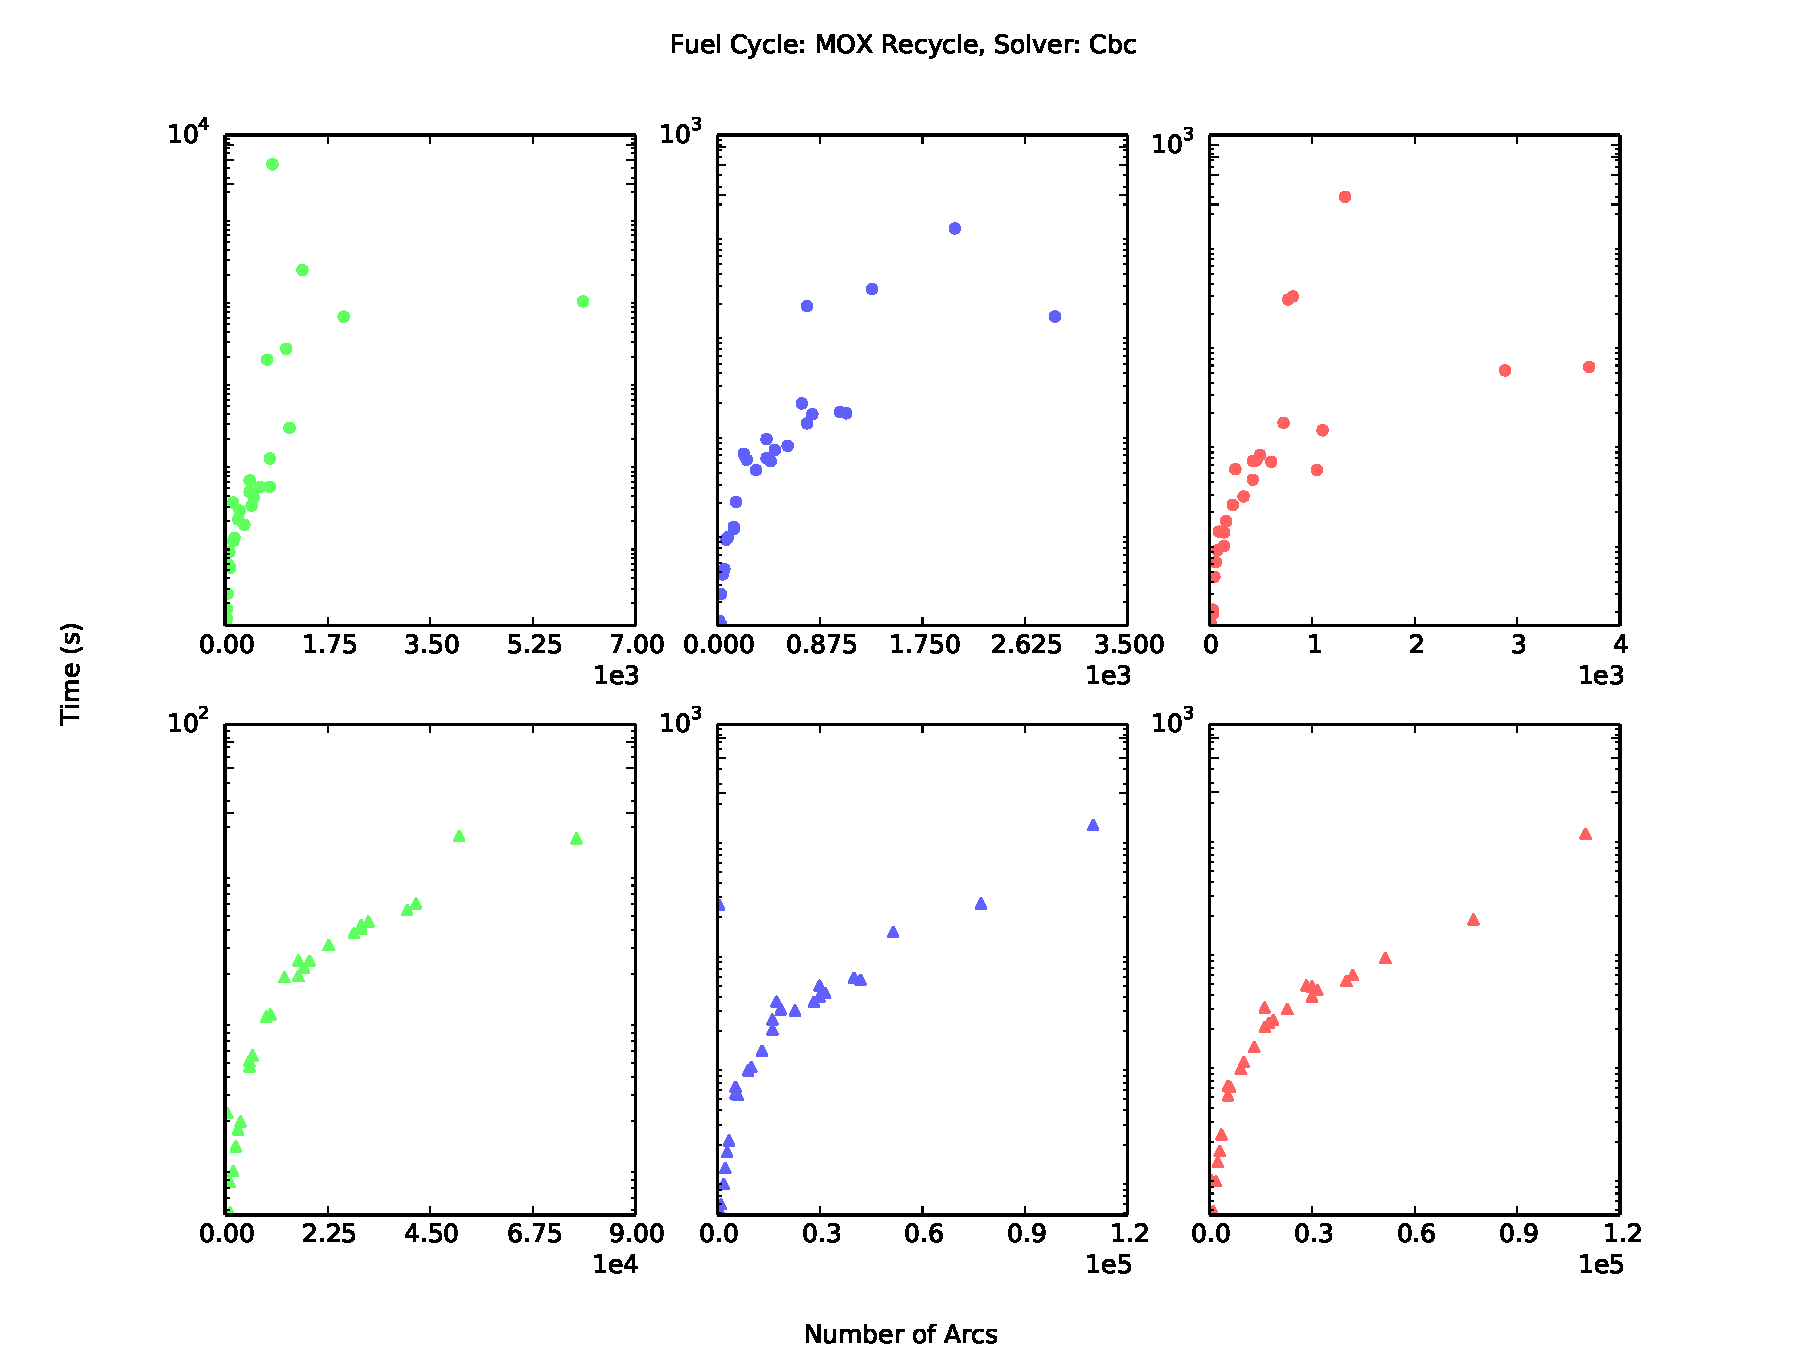
\includegraphics[width=.7\textwidth]{base_front_n_arcs_time_fc1_solvercbc.pdf}
    \caption[]{
      \label{fig:base_front_n_arcs_time_fc1_solvercbc}
      CBC Solver results for the MOX fuel cycle as the number of arcs
      increases.
      }
  \end{center}
\end{figure}

\begin{figure}[h!]
  \begin{center}
    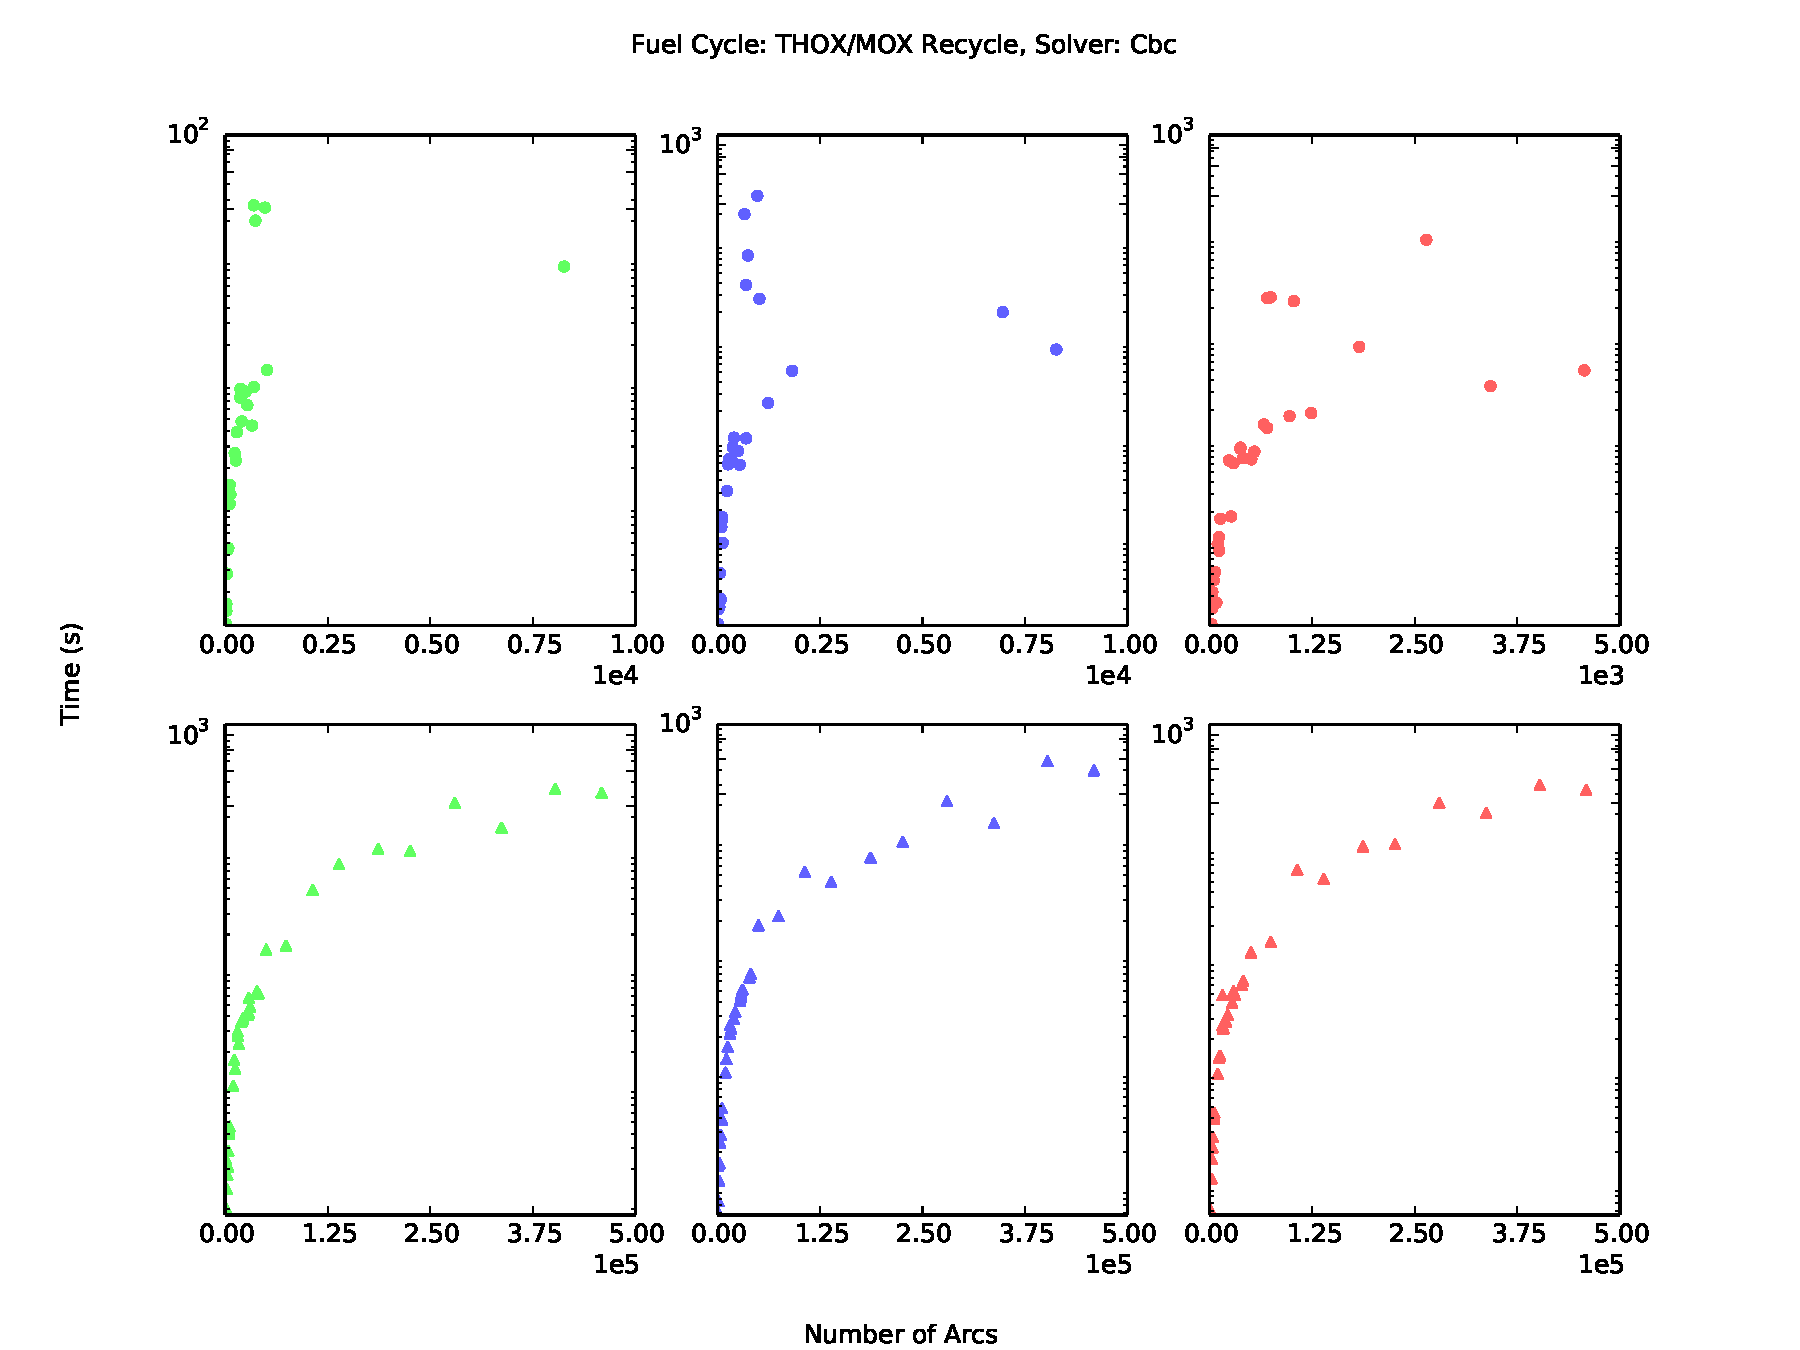
\includegraphics[width=.7\textwidth]{base_front_n_arcs_time_fc2_solvercbc.pdf}
    \caption[]{
      \label{fig:base_front_n_arcs_time_fc2_solvercbc}
      CBC Solver results for the ThOX fuel cycle as the number of arcs
      increases.
      }
  \end{center}
\end{figure}

Immediately obvious, and slightly counter intuitive, is that the population of
converged instances is larger for assembly-based exchanges rather than
batch-based exchanges, even though the number of variables in the problem is
much lower for batch-based exchanges. 

\TODO{More Explanation..}

%% \subsubsection{Instance Parameter Variation}
%% % Include large and small r_l_c

%% \paragraph{Location-to-Commodity Importance Ratio}

%% \paragraph{Thermal and Fast-Reactor Populations}

%% \paragraph{Inventory vs. Processing Constraints}

\subsubsection{Convergence Criteria}

The CBC solver is highly tuneable. Perhaps the most critical tuneable criteria
affecting the balance between solution quality and solution time is the
convergence criteria. It is not clear to what degree solution quality will
matter for users of Cyclus. Accordingly, a short exploratory experiment was
conducted to examine to what degree convergence criteria affects solution time.

CBC uses either an absolute or relative upper and lower-bound gap tolerance as
possible convergence criteria. This experiment uses the relative gap, termed
\textit{ratio gap} in CBC parlance. For each of the 18 combinations of
fundamental parameters, 10 instances of exchanges were executed, spanning a
reactor population range of 10 to 500. Figure \ref{fig:hist_front_rxtr_0}
displays the results for runs with reactors trading full batches for ratio gap
values of 0.1, 1, and 10\%. Figure \ref{fig:hist_front_rxtr_0} displays the
results for runs with reactors trading individual assemblies for ratio gap
values of 1 and 10\%.

\begin{figure}[h!]
  \begin{center}
    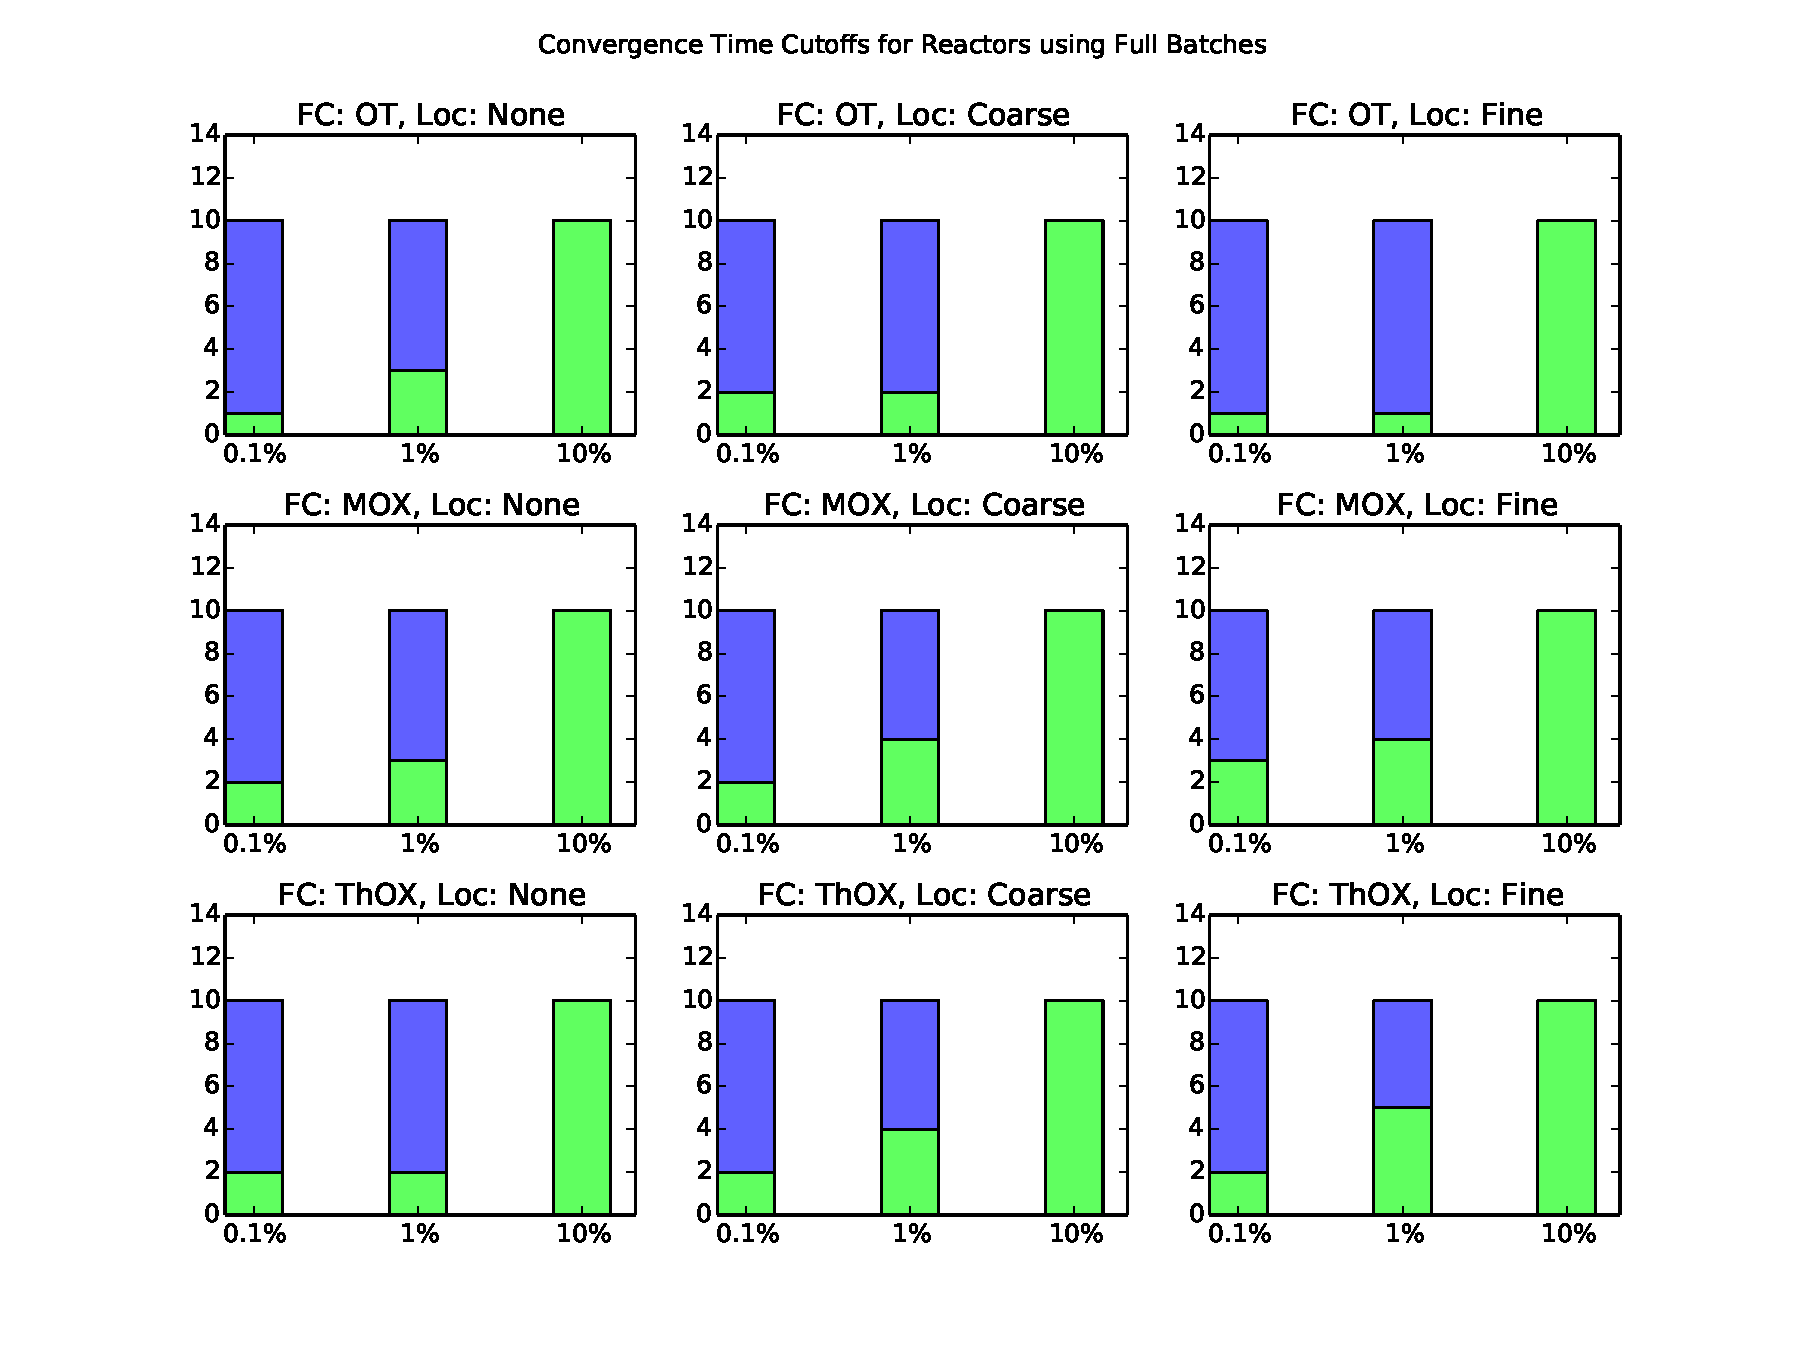
\includegraphics[width=.95\textwidth]{hist_front_rxtr_0.pdf}
    \caption[]{
      \label{fig:hist_front_rxtr_0}
      Effects of increasing convergence criteria on Front-End exchanges with
      reactors exchanging batches. Each bar is divided into how many instances
      converged (green) and did not converge (blue). }
  \end{center}
\end{figure}

\begin{figure}[h!]
  \begin{center}
    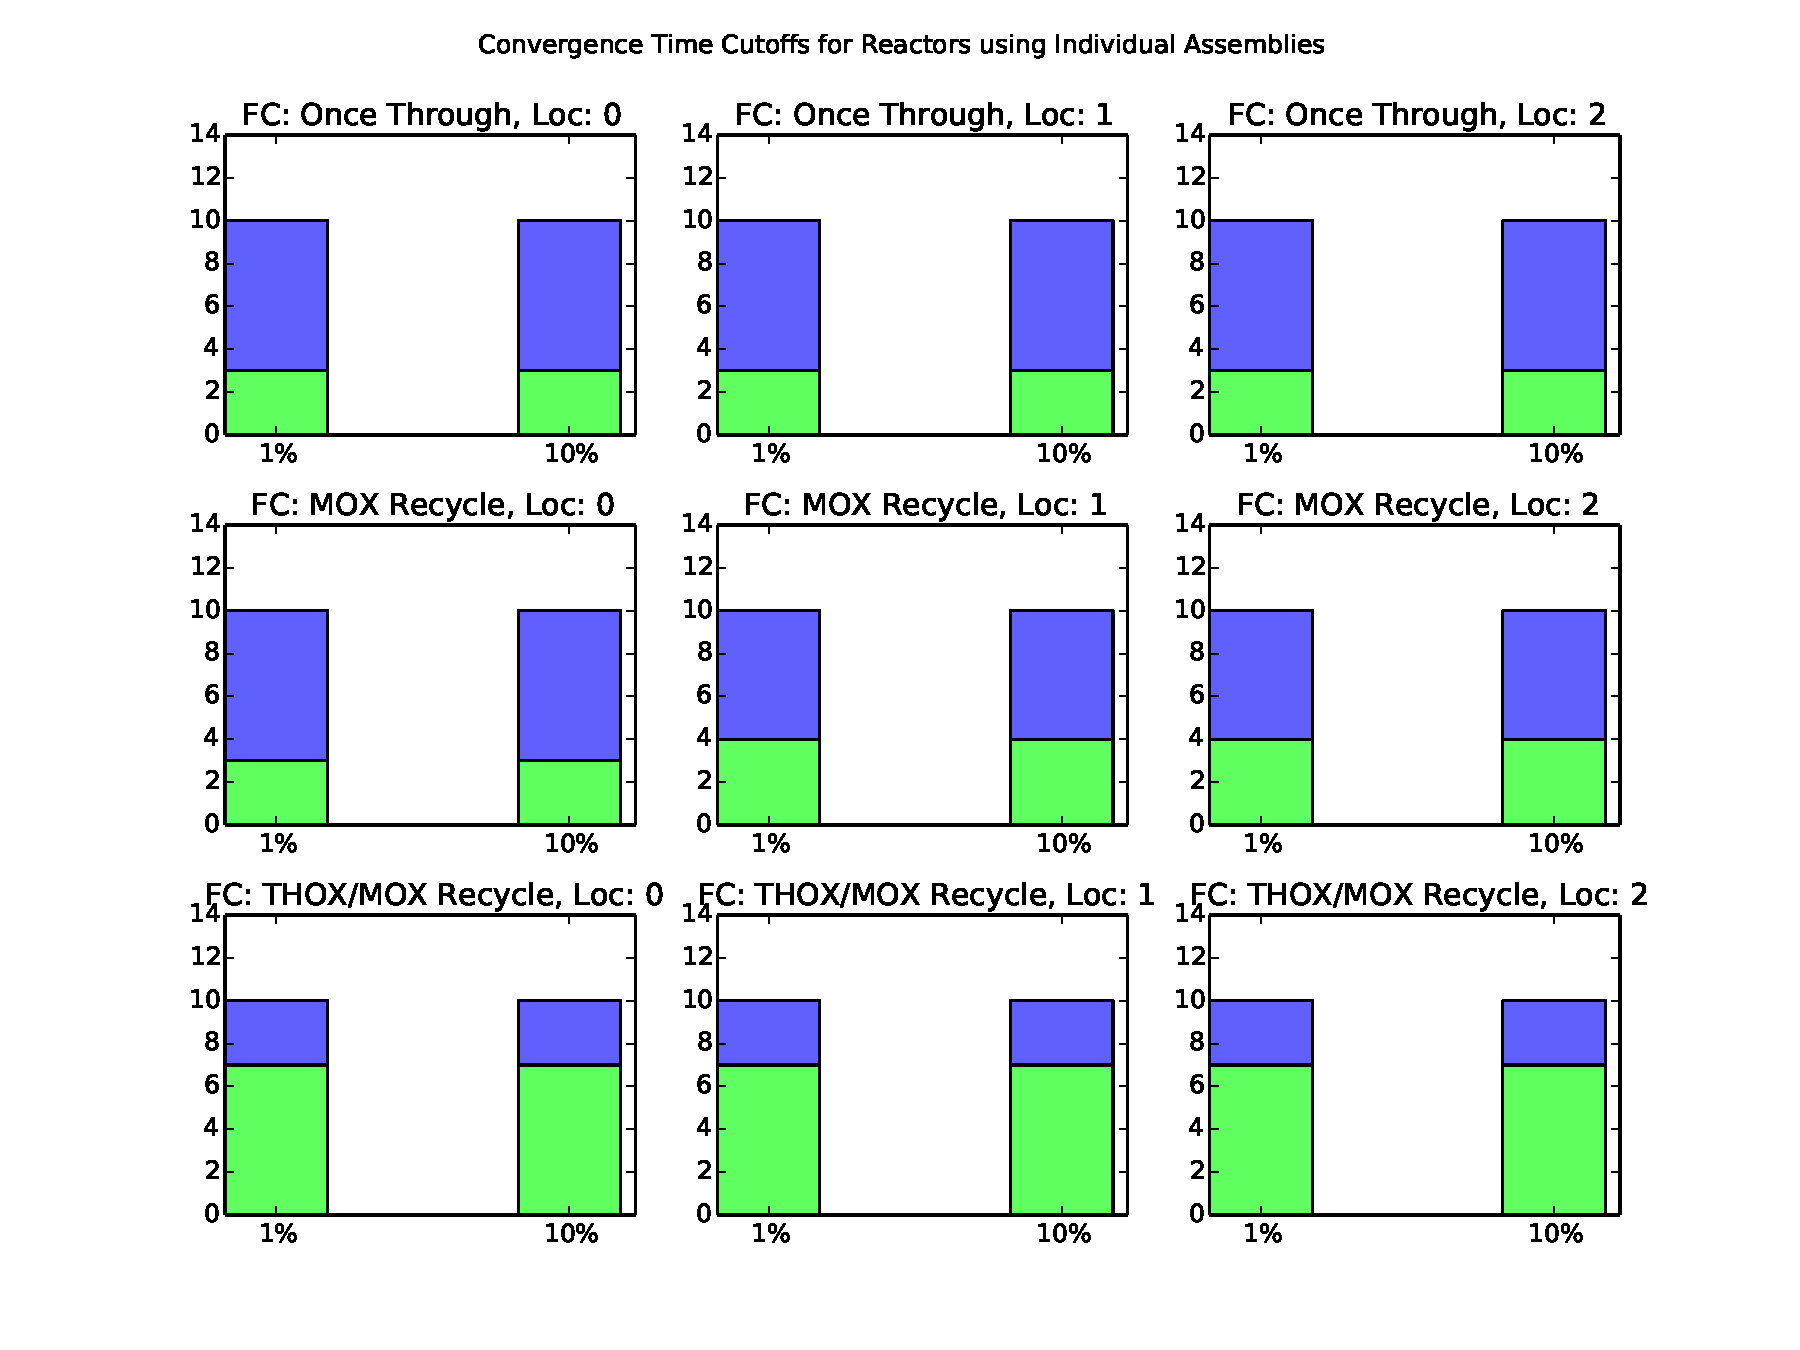
\includegraphics[width=.95\textwidth]{hist_front_rxtr_1.pdf}
    \caption[]{
      \label{fig:hist_front_rxtr_1}
      Effects of increasing convergence criteria on Front-End exchanges with
      reactors exchanging assemblies. Each bar is divided into how many instances
      converged (green) and did not converge (blue).}
  \end{center}
\end{figure}

Unsurprisingly, increasing the convergence criteria for smaller problems has a
greater effect than increasing the convergence criteria for larger probems. It
is somewhat surprising that the increase from a 1\% relative bound gap to a 10\%
gap allows full convergence in the smaller case and has no effect in the larger
case. Users will likely find some relaxation in convergence criteria will
provide speed ups in solution times, as expected. This result seems to indicate
that the relaxed convergence criteria will have a much more profound effect on
smaller problems.

\subsection{Back-End Exchanges}

\subsubsection{Reference Case}



%% \subsubsection{Instance Parameter Variation}
%% % Include large and small r_l_c

%% \paragraph{Location-to-Commodity Importance Ratio}

%% \paragraph{Thermal and Fast-Reactor Populations}

\subsubsection{Convergence Criteria}



\section{Stochastic Campaign}\label{results:stochastic}

The generation of exchanges is designed as a stochastic process. Each reactor is
assigned a target enrichment per consumable commodity in a given range. Further,
each facility is assigned a location value. Enrichment stochasticity results in
perturbed constraint matrix coefficients, and location stochasticity results in
perturbed objective coefficient if $f_{\text{loc}}$ is set to include
location-based preference.

In \secref{results:scale}, a single exchange instance was investigated for each
solver as problem size scale was investigated. While clear patterns were
inferred as a result of the study, stochastic effects were left
unexplored. Accordingly, a second study was undertaken in order to examine how
sensitive both solution values and execution time are to randomness in instance
generation.

For this study, instances are generated for a single parameter vector. It is
best to compare converged \cbc solutions for confidence in the resulting
objective value and in order to run all desired instances in a reasonable amount
of time. Accordingly, the total reactor population was set at 65 based on the
scaling study results. Specifically, this is approximately the largest reactor
population for which all configurations of parameters converged (see Figure
\ref{fig:base_front_n_rxtr_time_fc0_cbc}). For each combination of fundamental
parameters, 1000 instances were generated and executed by each solver for both
front and back-end exchanges.

In both sections, cumulative observations are presented. Figures are presented
in two panes for a given fuel cycle, with low-fidelity reactor instances on the
left and high-fidelity reactor instances on the right. In each pane, the results
for all three location fidelity parameters are shown.

\subsection{Front-End Exchanges}

\subsubsection{Fundamental Parameter Variation}

The Greedy Solver and CLP both proved to have relatively stable solution
times. The timing results are similar across fuel cycles. Accordingly, MOX fuel
cycle results are shown for the Greedy Solver in Figure
\ref{fig:1k_avg_front_time_fc1_greedy}, and CLP results are shown in Figure
\ref{fig:1k_avg_front_time_fc1_clp}. Apart from solution time stability, the
primary observation for both the CLP and Greedy solvers is related to location
fidelity effects. Although there is a ranking in average solution time by
location parameter \textit{for a given collection of fundamental parameters},
that ranking changes for each collection of parameters, as can be seen in the
presented figures.

\begin{figure}[h!]
  \begin{center}
    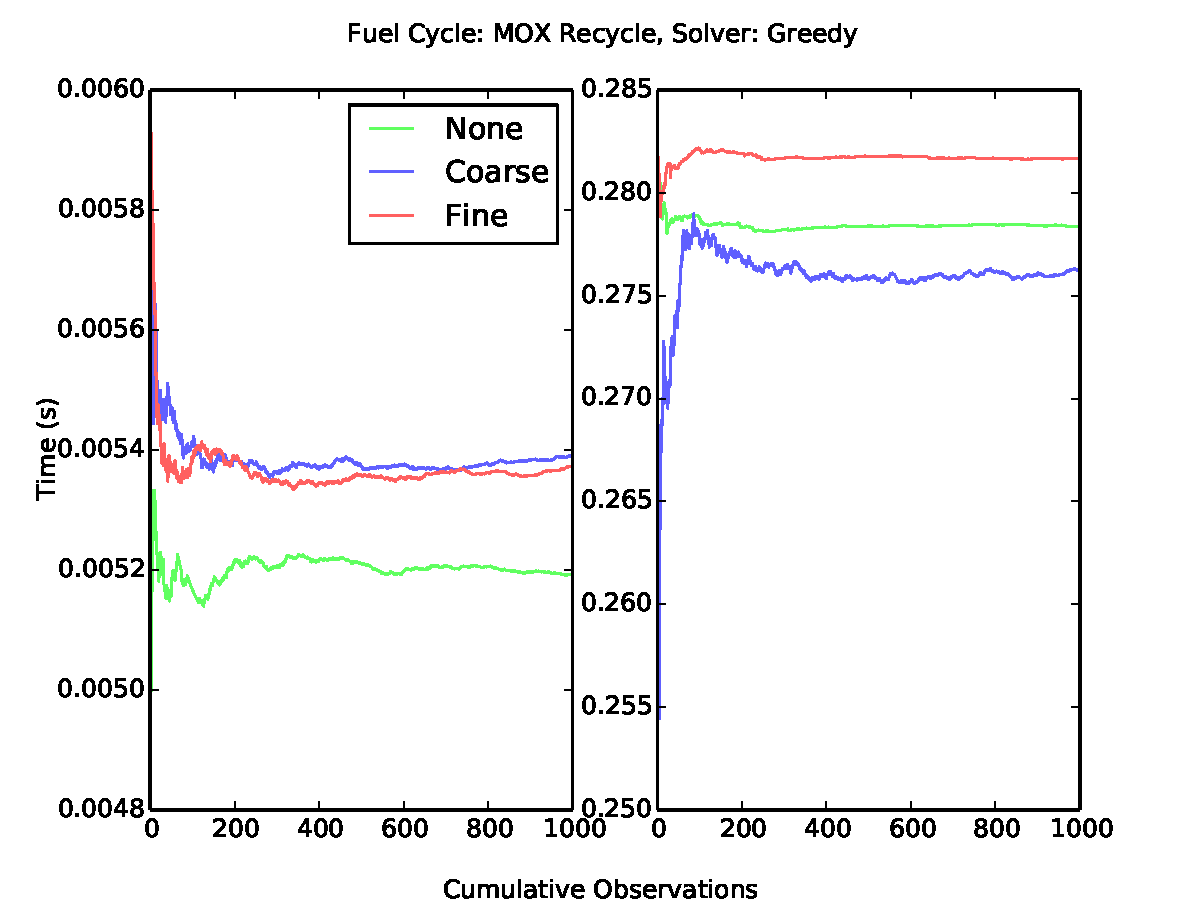
\includegraphics[width=.7\textwidth]{1k_avg_front_time_fc1_greedy.pdf}
    \caption{
      \label{fig:1k_avg_front_time_fc1_greedy}
      Cumulative average solution time of the Greedy solver for the front-end
      MOX fuel cycle. Low-fidelity reactor instances comprise the left pane, and
      high-fidelity reactor instances comprise the right pane. Each colored line
      represents a different objective coefficient location fidelity.}
  \end{center}
\end{figure}

\begin{figure}[h!]
  \begin{center}
    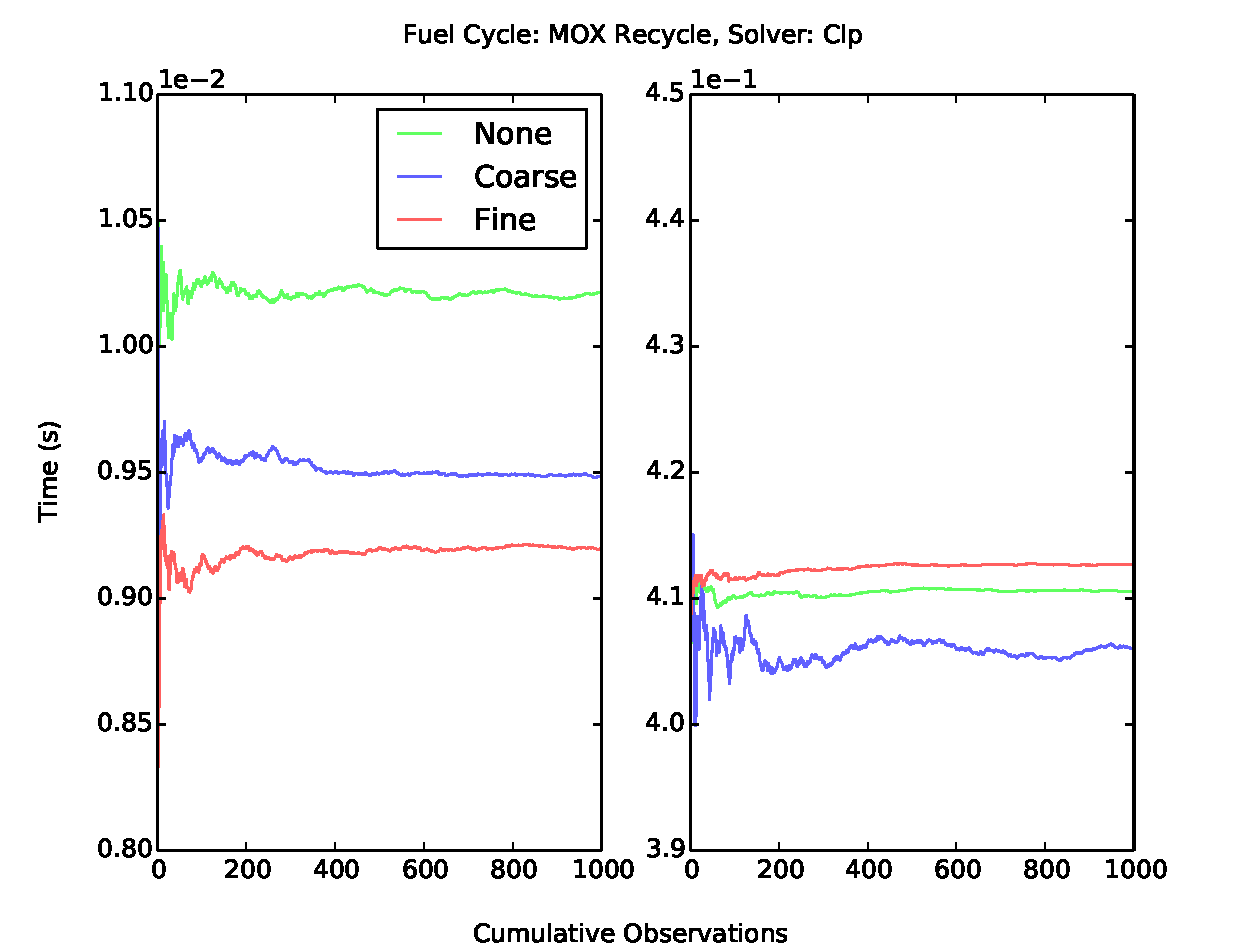
\includegraphics[width=.7\textwidth]{1k_avg_front_time_fc1_clp.pdf}
    \caption{
      \label{fig:1k_avg_front_time_fc1_clp}
      Cumulative average solution time of the \clp solver for the front-end MOX fuel
      cycle.}
  \end{center}
\end{figure}

The \cbc solver showed much less stability in solution times. Further, behavior
was found to be different for each fuel
cycle. \Cref{fig:1k_avg_front_time_fc0_cbc,fig:1k_avg_front_time_fc1_cbc,fig:1k_avg_front_time_fc2_cbc}
show the timing results for the OT, MOX, and ThOX fuel cycles,
respectively. 

\begin{figure}[h!]
  \begin{center}
    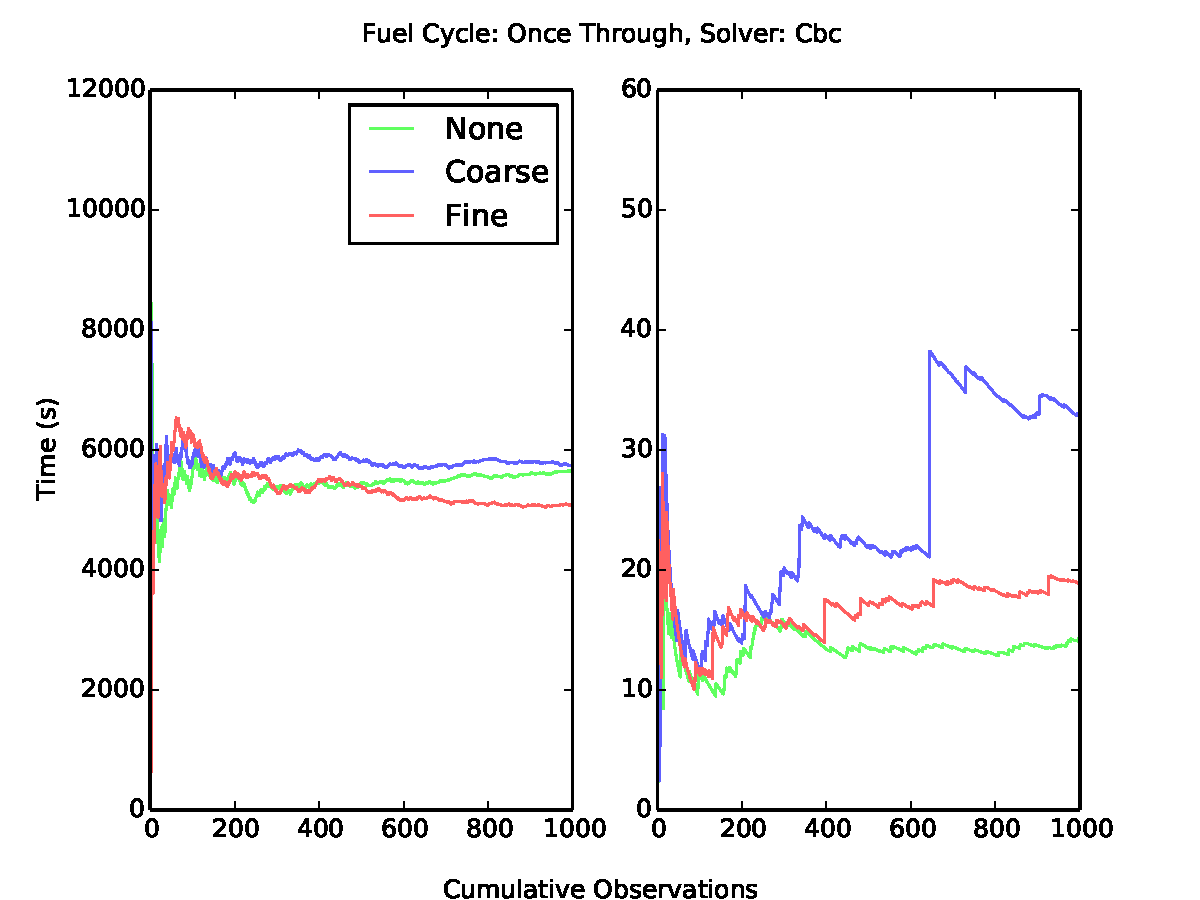
\includegraphics[width=.7\textwidth]{1k_avg_front_time_fc0_cbc.pdf}
    \caption{
      \label{fig:1k_avg_front_time_fc0_cbc}
      Cumulative average solution time of the \cbc solver for the front-end
      once-through fuel cycle.}
  \end{center}
\end{figure}

\begin{figure}[h!]
  \begin{center}
    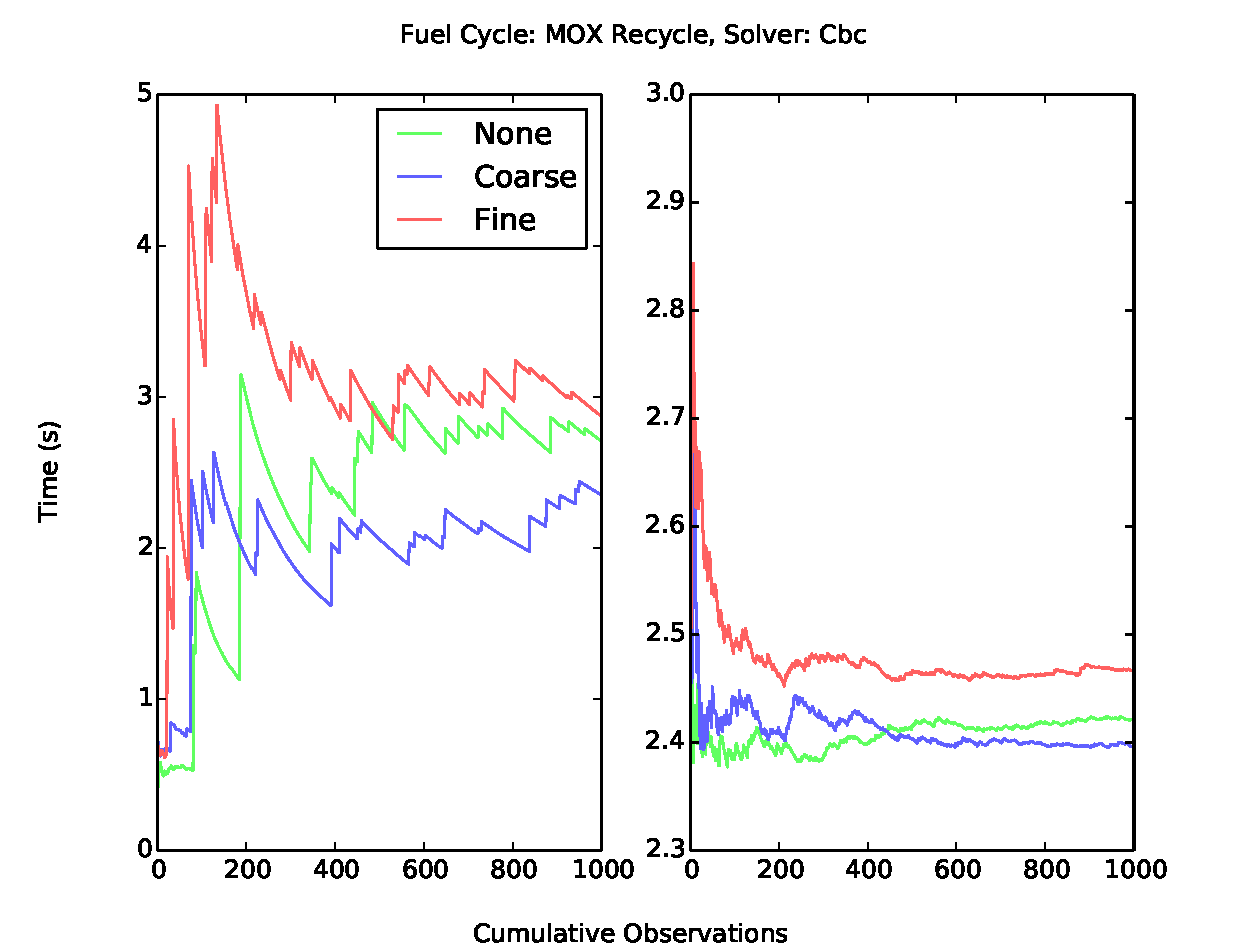
\includegraphics[width=.7\textwidth]{1k_avg_front_time_fc1_cbc.pdf}
    \caption{
      \label{fig:1k_avg_front_time_fc1_cbc}
      Cumulative average solution time of the \cbc solver for the front-end MOX
      fuel cycle.}
  \end{center}
\end{figure}

\begin{figure}[h!]
  \begin{center}
    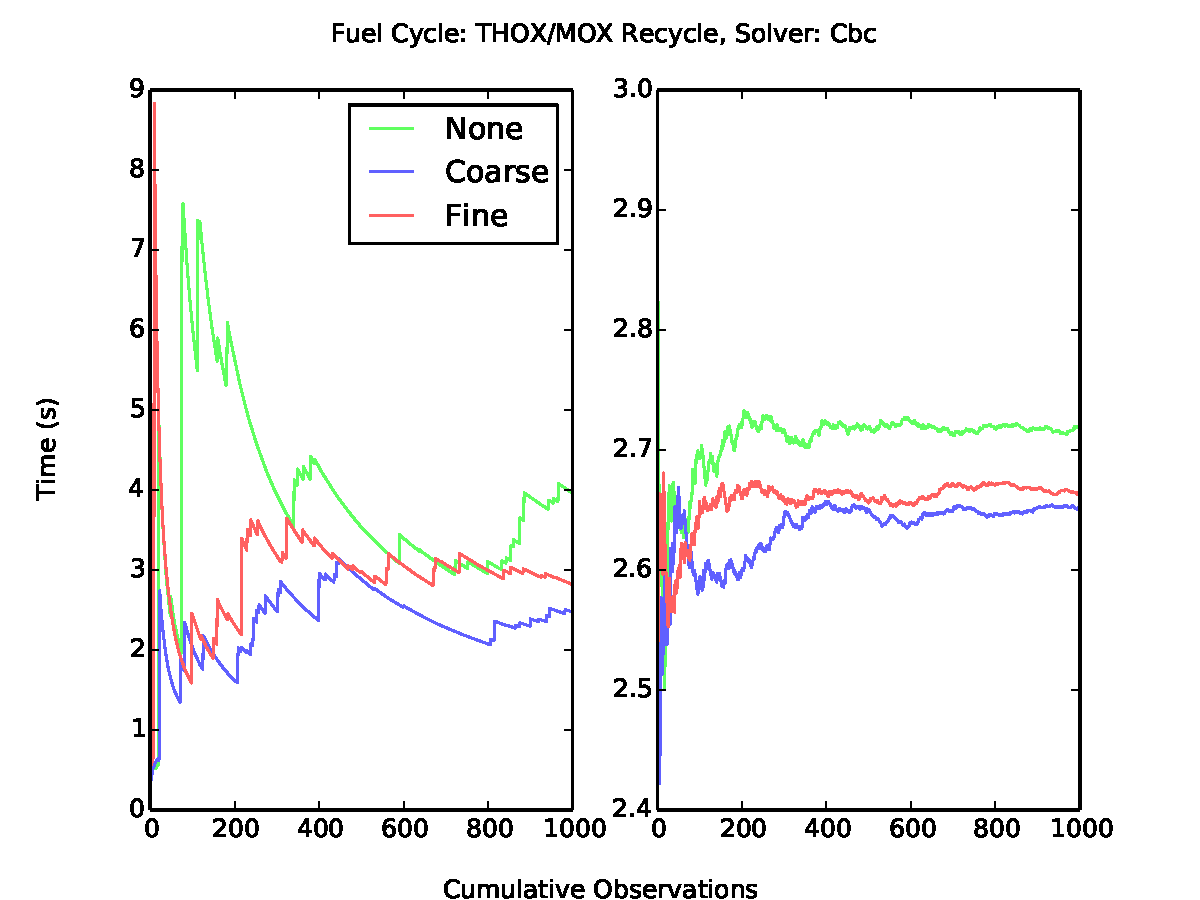
\includegraphics[width=.7\textwidth]{1k_avg_front_time_fc2_cbc.pdf}
    \caption{
      \label{fig:1k_avg_front_time_fc2_cbc}
      Cumulative average solution time of the \cbc solver for the front-end ThOX
      fuel cycle.}
  \end{center}
\end{figure}

Given the variety in stability by fuel cycle, viewing the underlying timing
distributions can also provide insight. Accordingly, Figure
\ref{fig:1k_hist_front_rx0} shows all timing distributions for low-fidelity
reactor models, and Figure \ref{fig:1k_hist_front_rx1} displays the
corresponding results for high-fidelity models.

\begin{figure}[h!]
  \begin{center}
    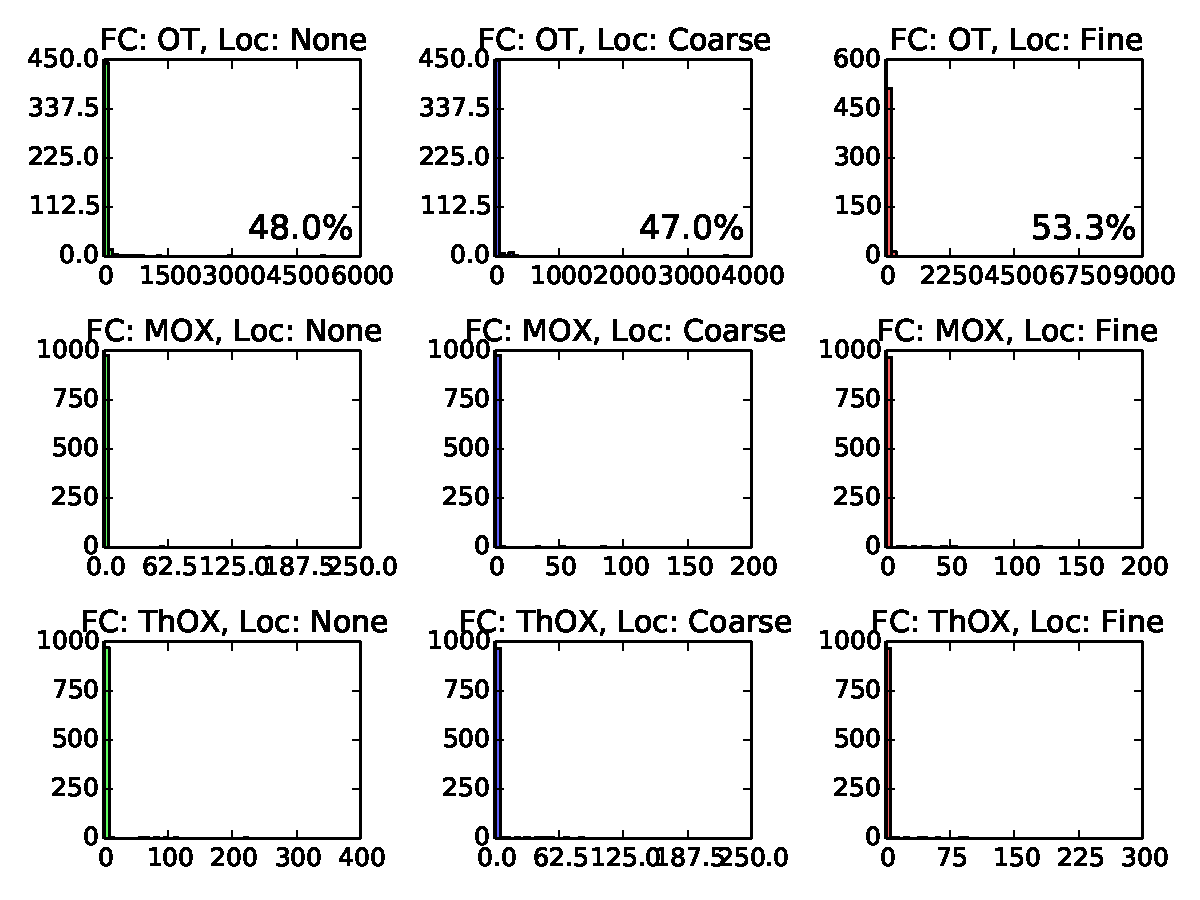
\includegraphics[width=.7\textwidth]{1k_hist_front_rx0.pdf}
    \caption{
      \label{fig:1k_hist_front_rx0}
      The distribution of converged solution times for all low-fidelity reactor
      instances. Fuel cycle fidelity increases from top to bottom, and location
      fidelity increases from right to left. Percentages of converged instances
      are provided if relevant.}
  \end{center}
\end{figure}

\begin{figure}[h!]
  \begin{center}
    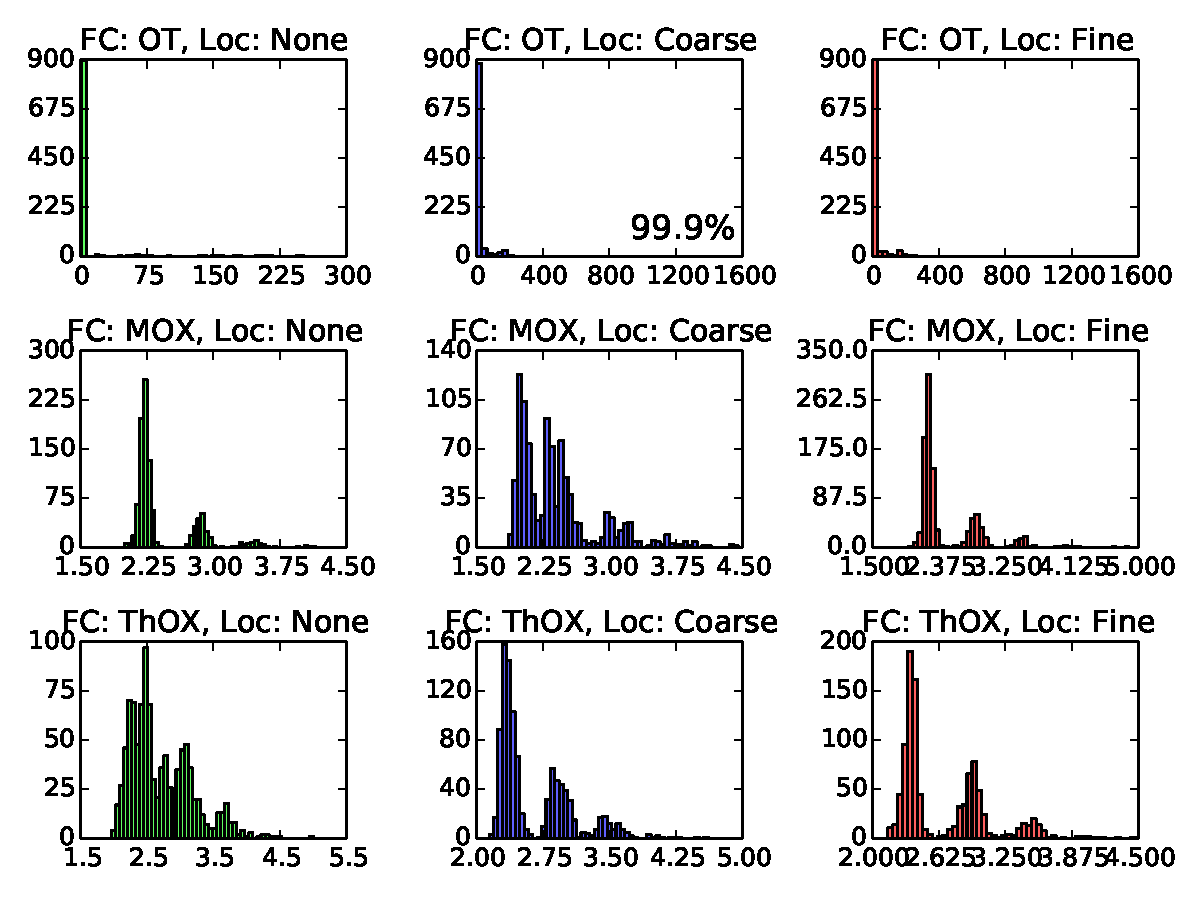
\includegraphics[width=.7\textwidth]{1k_hist_front_rx1.pdf}
    \caption{
      \label{fig:1k_hist_front_rx1}
      The distribution of converged solution times for all high-fidelity reactor
      instances. Fuel cycle fidelity increases from top to bottom, and location
      fidelity increases from right to left. Percentages of converged instances
      are provided if relevant.}
  \end{center}
\end{figure}

A number of interesting features exist in the figures related to the \cbc timing
study. Significantly, reactors in batch-mode have poor convergence for
once-through cycles, regardless of location parameter. This echoes
observations in the scaling study. For the remaining fuel cycles, outliers
consistently are observed for low-fidelity reactor models, also regardless of
location parameter. This effect is seen in the cumulative observation figures
most easily. Each occurrence of a timing outlier causes a large jump in the
observation. 

Conversely, high-fidelity reactor instances were found to almost always
converge. Outliers were found to dominate the once-through fuel cycle
results. Again, this behavior results in choppy cumulative observations. Both
the MOX and ThOX fuel cycles were shown to be comparatively stable. Further,
their solution time distributions proved to have some structure. It is not clear
why these combinations of fundamental parameters result in such structure.

\subsubsection{Simulation Objective vs. Solution Time}

The trade off of choosing to use a full-fledged optimization solver over a
heuristic is one between solution fidelity and solution time. Figure
\ref{fig:1k_compare_front_pref_flow} shows a comparison between the \cbc and
Greedy solvers. For each instance, relative simulation-objective values were
computed as shown in Equation \ref{eqn:sim_flow_compare}. Similarly, relative
solution times were computed. The average result found for high-fidelity reactor
instances solved with \cbc was taken as a reference point, plotted at the origin
in Figure \ref{fig:1k_compare_front_pref_flow}. Values are plotted for each
combination of fundamental parameters. A data point's position along the x-axis
indicates the average deviation from the high-fidelity model's simulation
objective, i.e., the dot product of preference and system flow. The y-axis
position indicates the average relative time difference.

\begin{figure}[h!]
  \begin{center}
    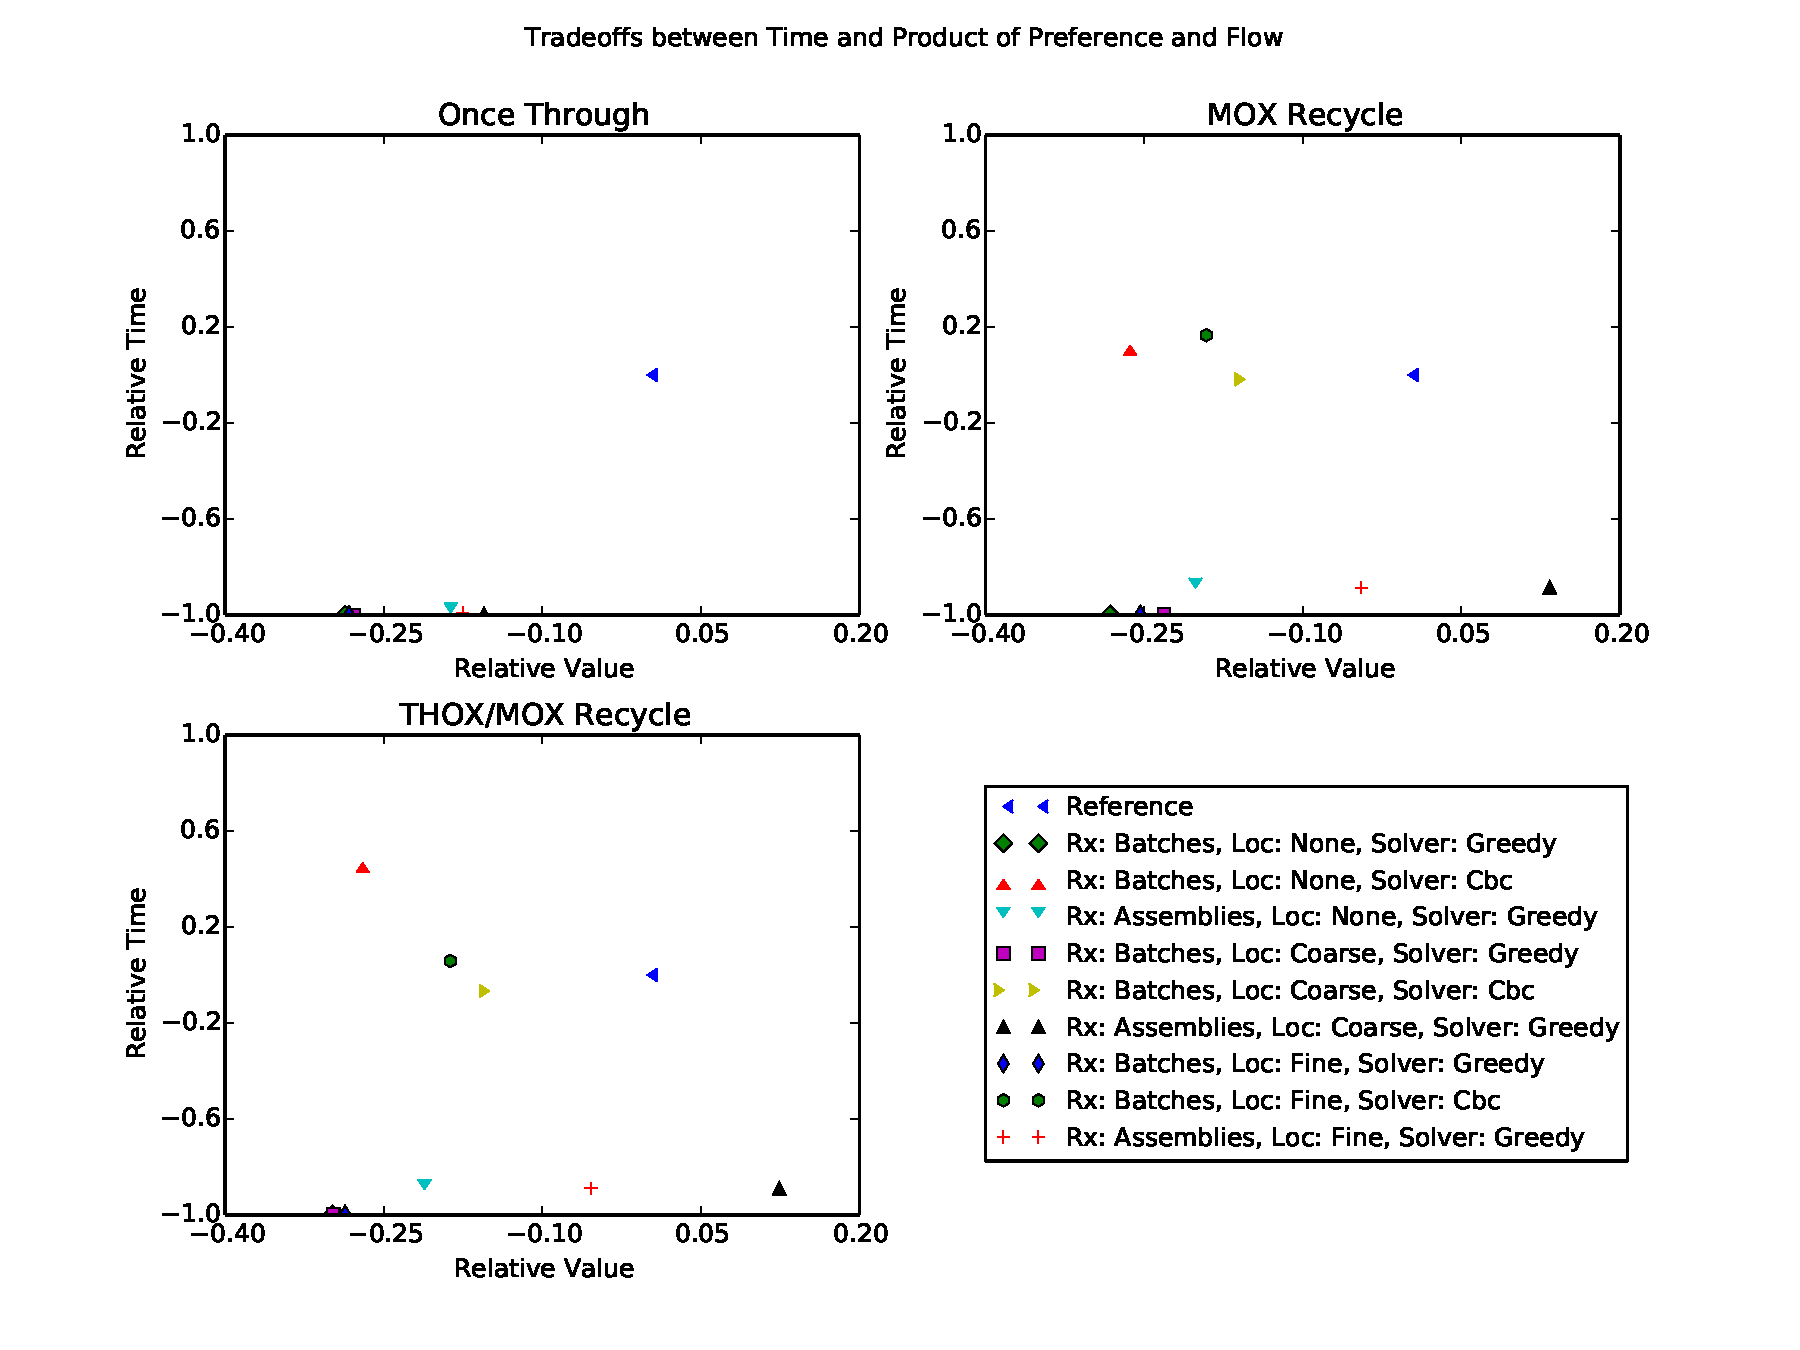
\includegraphics[width=.7\textwidth]{1k_compare_front_pref_flow.pdf}
    \caption{
      \label{fig:1k_compare_front_pref_flow}
      A comparison of simulation-objective values and solution times between
      instances solved with Greedy and \cbc solvers. Reference values are
      comprised of high-fidelity reactor instances solved with \cbc. Each other
      combination of fundamental parameter and solvers are then compared agaisnt
      the reference. Note that the once-through fuel cycle pane does not include
      other \cbc solvers, because their solution times were very long.
    }
  \end{center}
\end{figure}

In most every case, the results are as expected. The high-fidelity, \cbc-based
solution provides a better simulation objective for a more expensive time. In
general, the Greedy always performs much faster than \cbc, as expected from a
heuristic. Except for the Once-through case, all \cbc solves require similar
times, and the highest fidelity simulation provides the answer with the highest
objective measure. However, as was seen in the scalability study, the \cbc does
not always provide a better simulation-based metric when large costs are
concerned. Interestingly, the coarse-location fidelity Greedy solver results
provided a better average simulation objective.

\subsubsection{False Arc Cost Effects}

As was shown for previously, providing a small pseudo cost results in a higher
simulation-based objective metric. For example, Figure
\ref{fig:1k_compare_front_pref_flow} displayed results in which the Greedy
solver provided a higher average simulation-based metric than the \cbc
solver. Figure \ref{fig:cost_avg_front_pref_flow_fc1_} displays the underlying
data with additional data for small-cost \cbc solves. As can be seen, in the
lower center pane, the average preference-flow metric increases in a
\cbc-high-cost, Greedy, \cbc-low-cost order.

\begin{figure}[h!]
  \begin{center}
    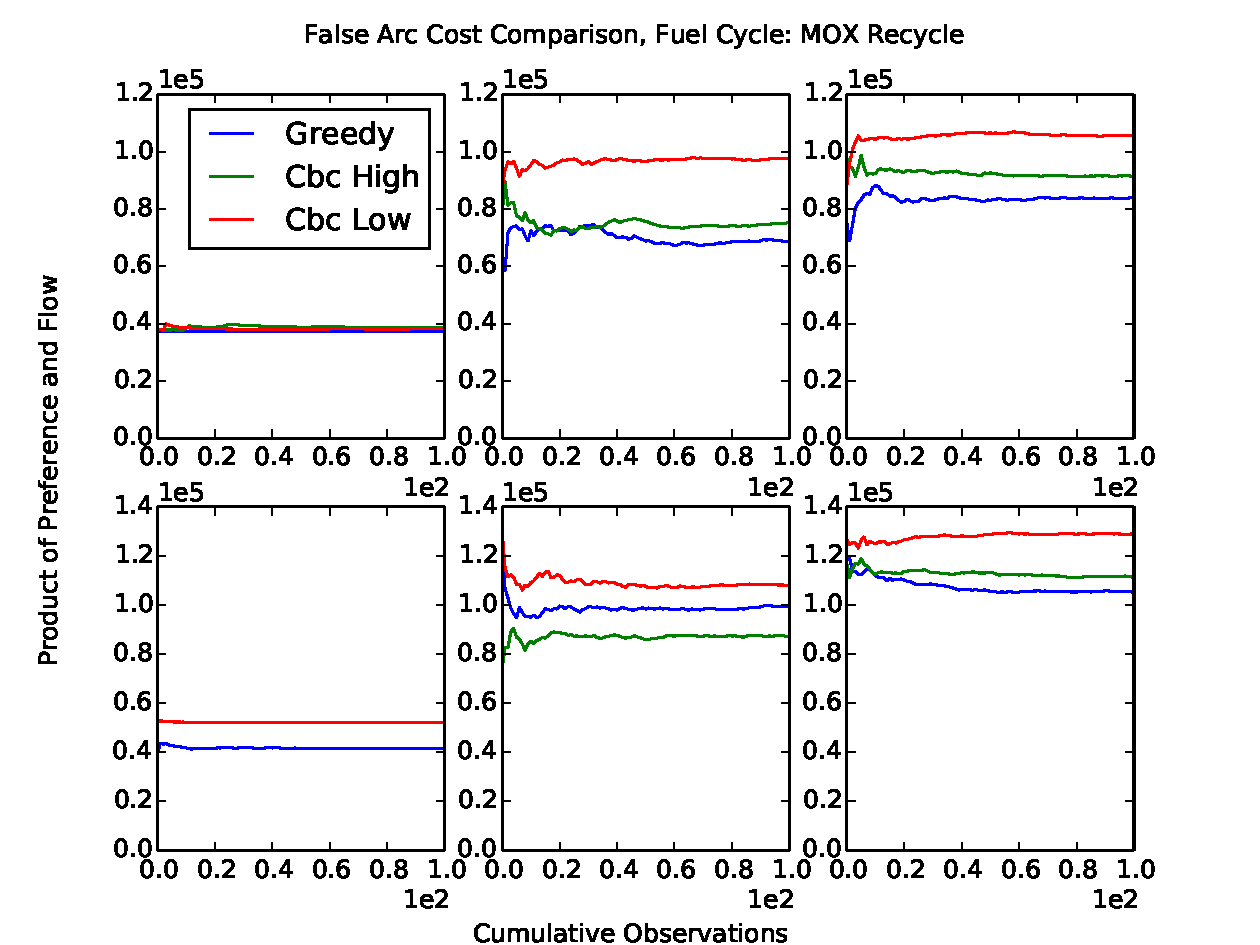
\includegraphics[width=.7\textwidth]{cost_avg_front_pref_flow_fc1_.pdf}
    \caption{
      \label{fig:cost_avg_front_pref_flow_fc1_}
      Simulation-objective values for 100 instances solved with the Greedy
      solver, a \cbc solver with a high false arc cost, and the \cbc solver with a
      low false arc cost.}
  \end{center}
\end{figure}

%% \subsubsection{Preference Conditioning Effects}

%% The relative weight provided to location over commodity preference does not
%% affect solution time.

%% \begin{figure}[h!]
%%   \begin{center}
%%     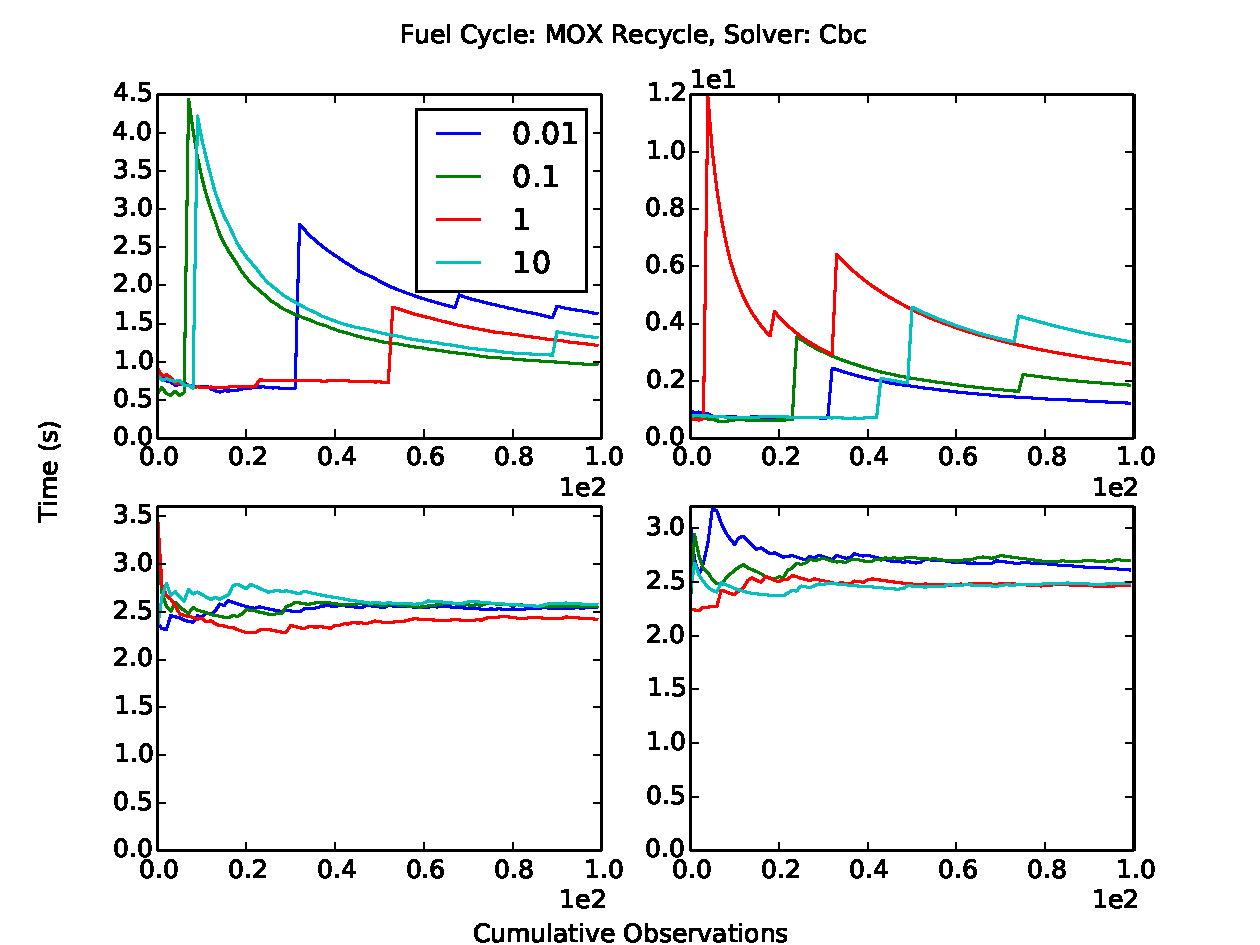
\includegraphics[width=.7\textwidth]{rlc_avg_front_time_fc1_cbc.pdf}
%%     \caption{
%%       \label{fig:rlc_avg_front_time_fc1_cbc}
%%       Caption.}
%%   \end{center}
%% \end{figure}

\subsection{Back-End Exchanges}

As with the scalability study, back-end exchanges perform quite similarly to
front-end exchanges. Accordingly, basic results are reviewed, and results that
lead to recommendations are discussed in more detail.

%% \subsubsection{Fundamental Parameter Variation}

Both the Greedy and \clp solvers again proved to have relatively stable solution
times. An example of the Greedy solver observed solution times for the MOX fuel
cycle is shown in Figure \ref{fig:1k_avg_back_time_fc1_greedy}. \clp results are
shown in Figure \ref{fig:1k_avg_back_time_fc1_clp}. 

\begin{figure}[h!]
  \begin{center}
    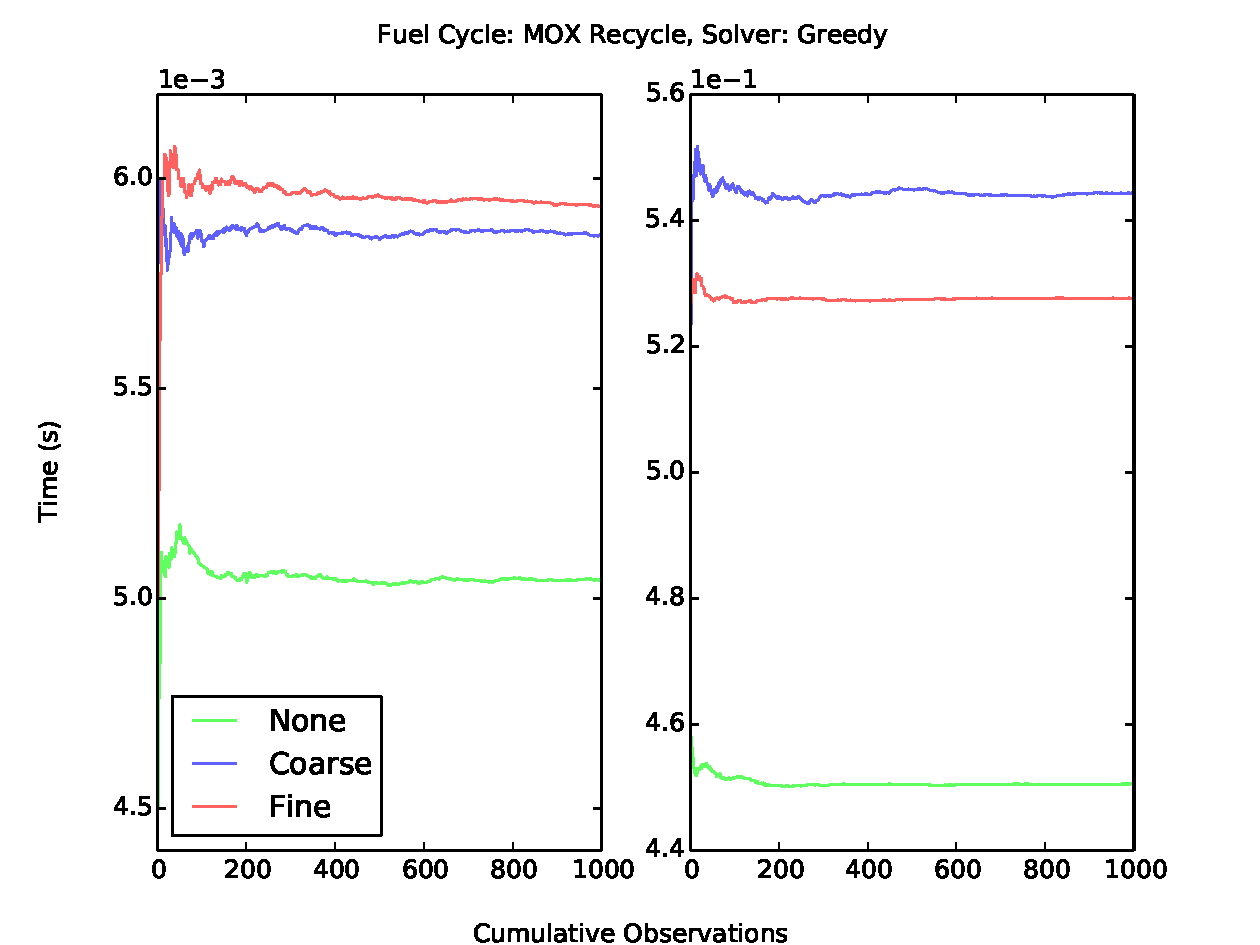
\includegraphics[width=.7\textwidth]{1k_avg_back_time_fc1_greedy.pdf}
    \caption{
      \label{fig:1k_avg_back_time_fc1_greedy}
      Cumulative average solution time of the Greedy solver for the back-end MOX
      fuel cycle.}
  \end{center}
\end{figure}

\begin{figure}[h!]
  \begin{center}
    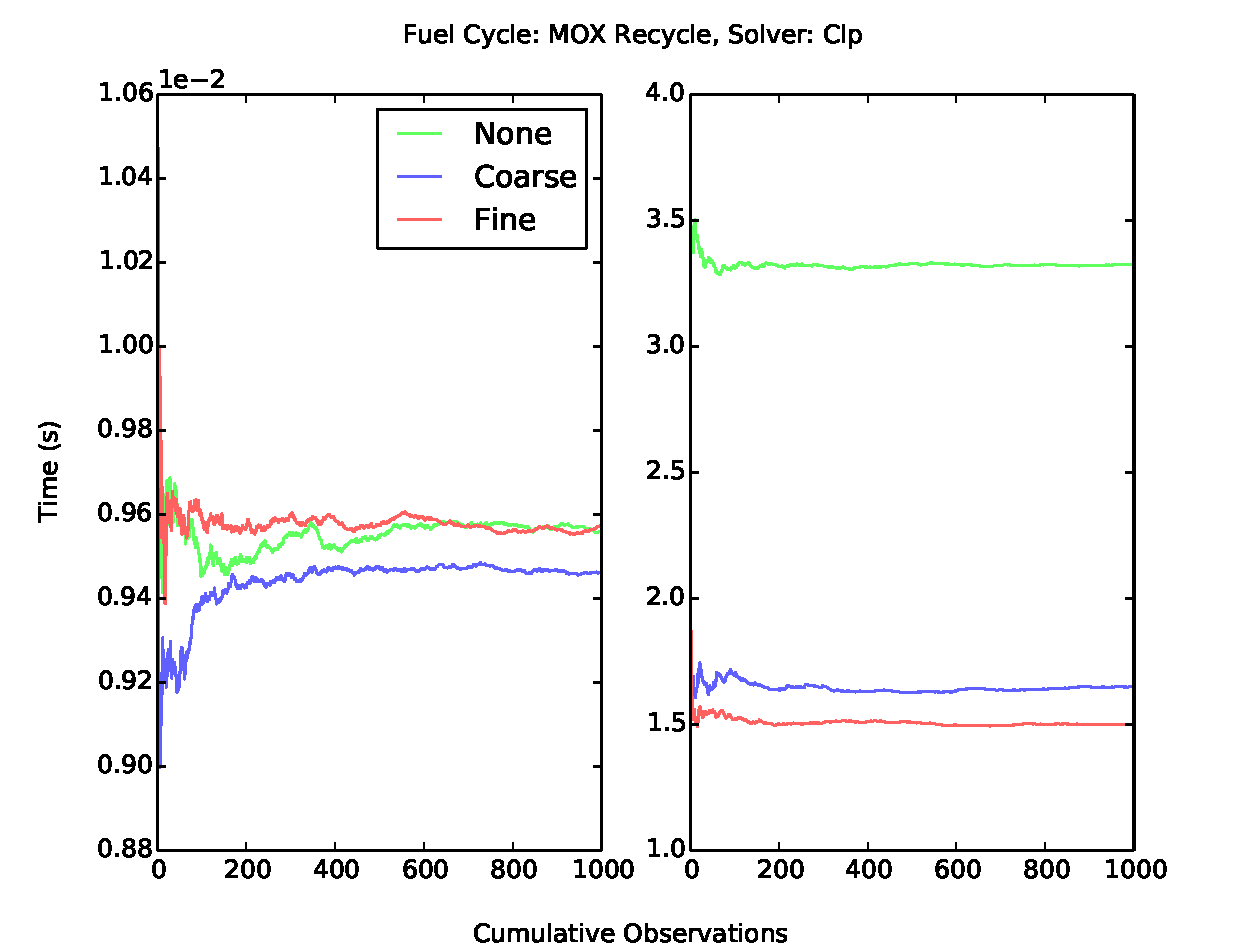
\includegraphics[width=.7\textwidth]{1k_avg_back_time_fc1_clp.pdf}
    \caption{
      \label{fig:1k_avg_back_time_fc1_clp}
      Cumulative average solution time of the \clp solver for the back-end MOX
      fuel cycle.}
  \end{center}
\end{figure}

The \clp solution time required for high-fidelity reactor models with no location
preference was found to be significantly higher than for instances which
included a location preference. A similar trend was found for \cbc solutions, as
shown in \Cref{fig:1k_avg_back_time_fc1_cbc,fig:1k_avg_back_time_fc2_cbc} for
the MOX and ThOX fuel cycles, respectively. While the timing discrepancy exists
in low-fidelity reactor models in the \cbc case, rather than high-fidelity, it is
also much more pronounced. These results indicate that solution times, in
certain instances, can be significantly reduced if solvers can better
differentiate between arcs based on objective coefficients. Therefore, a
possible speed-up strategy can include ``salting'' the preference vector by
adding a random $\delta_p$ to each entry.

\begin{figure}[h!]
  \begin{center}
    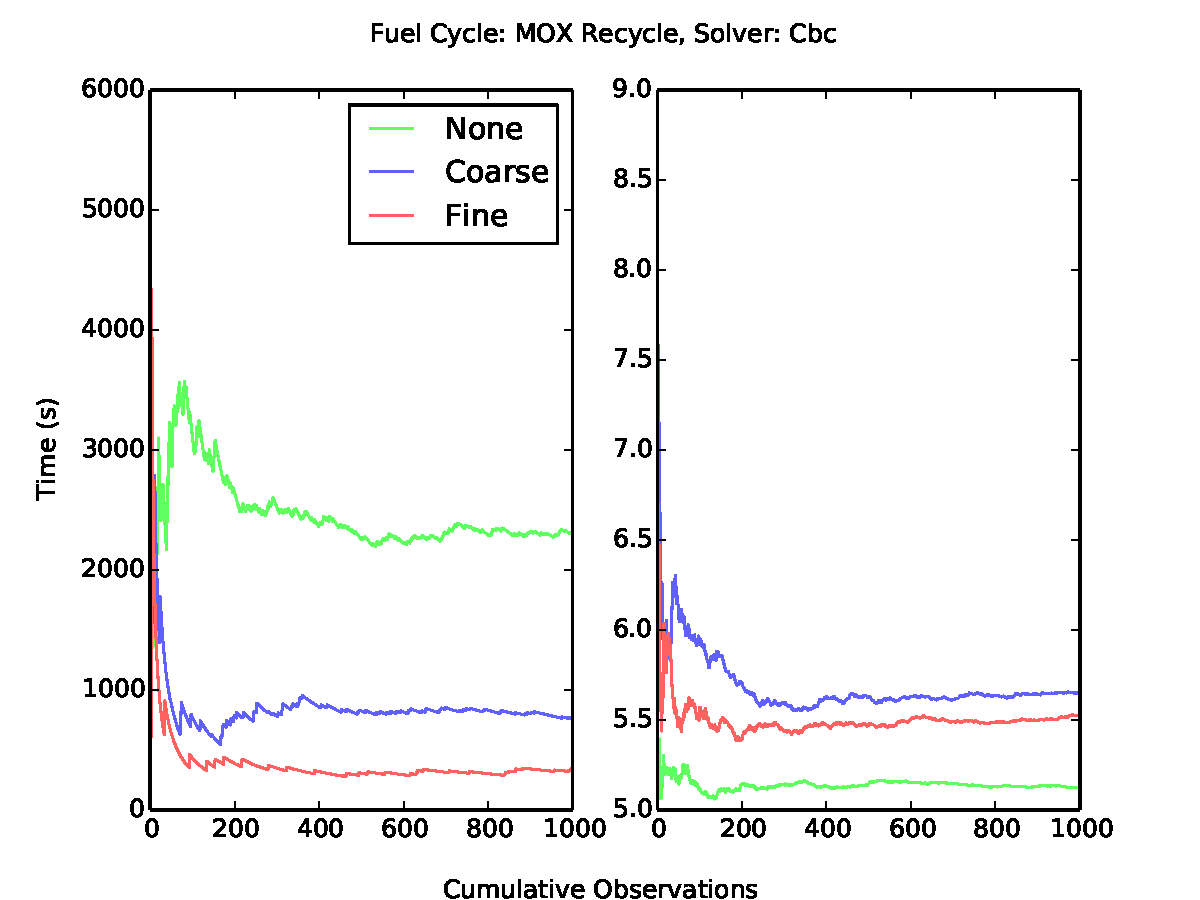
\includegraphics[width=.7\textwidth]{1k_avg_back_time_fc1_cbc.pdf}
    \caption{
      \label{fig:1k_avg_back_time_fc1_cbc}
      Cumulative average solution time of the \cbc solver for the back-end MOX
      fuel cycle.}
  \end{center}
\end{figure}

\begin{figure}[h!]
  \begin{center}
    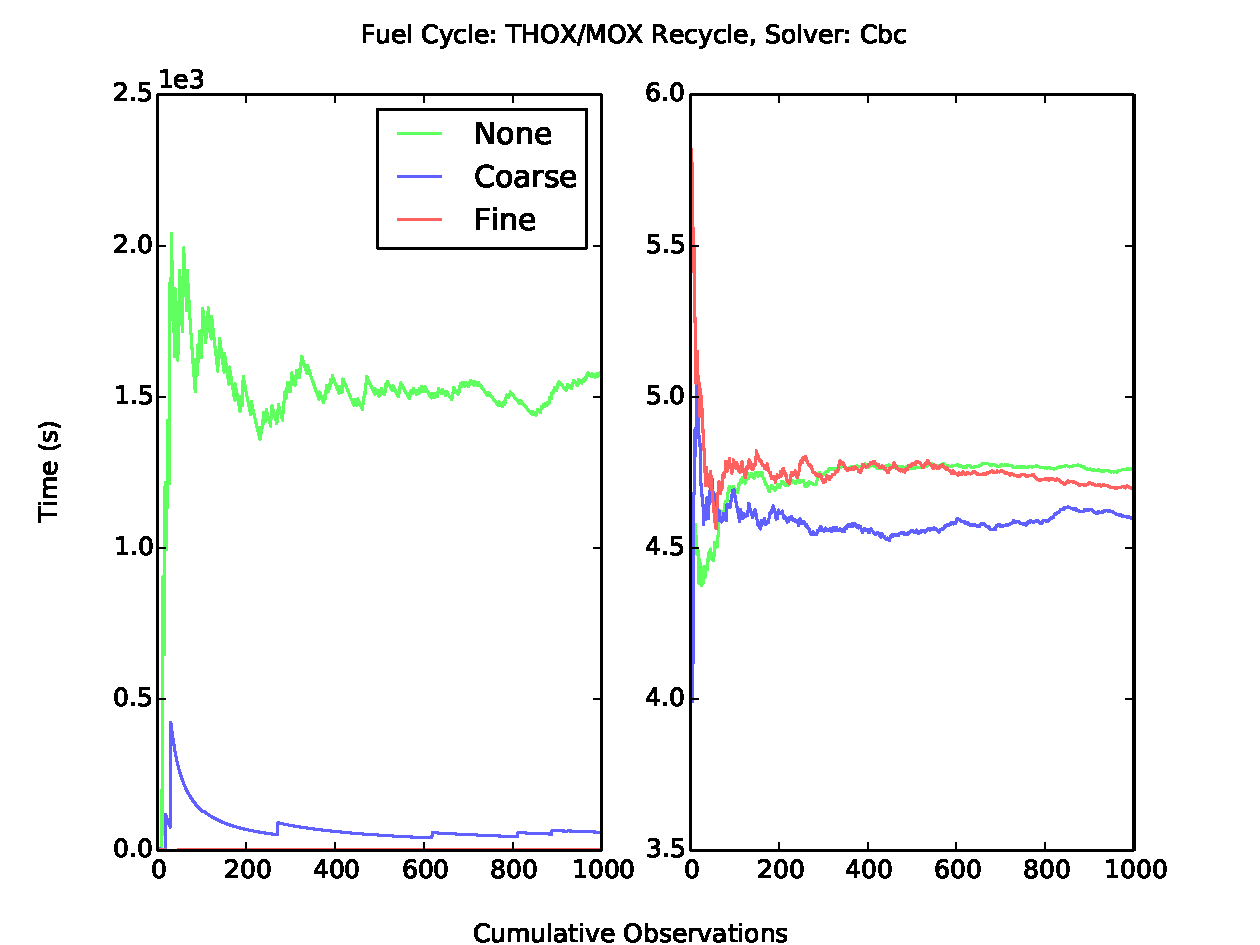
\includegraphics[width=.7\textwidth]{1k_avg_back_time_fc2_cbc.pdf}
    \caption{
      \label{fig:1k_avg_back_time_fc2_cbc}
      Cumulative average solution time of the \cbc solver for the back-end ThOX
      fuel cycle.}
  \end{center}
\end{figure}

%% \begin{figure}[h!]
%%   \begin{center}
%%     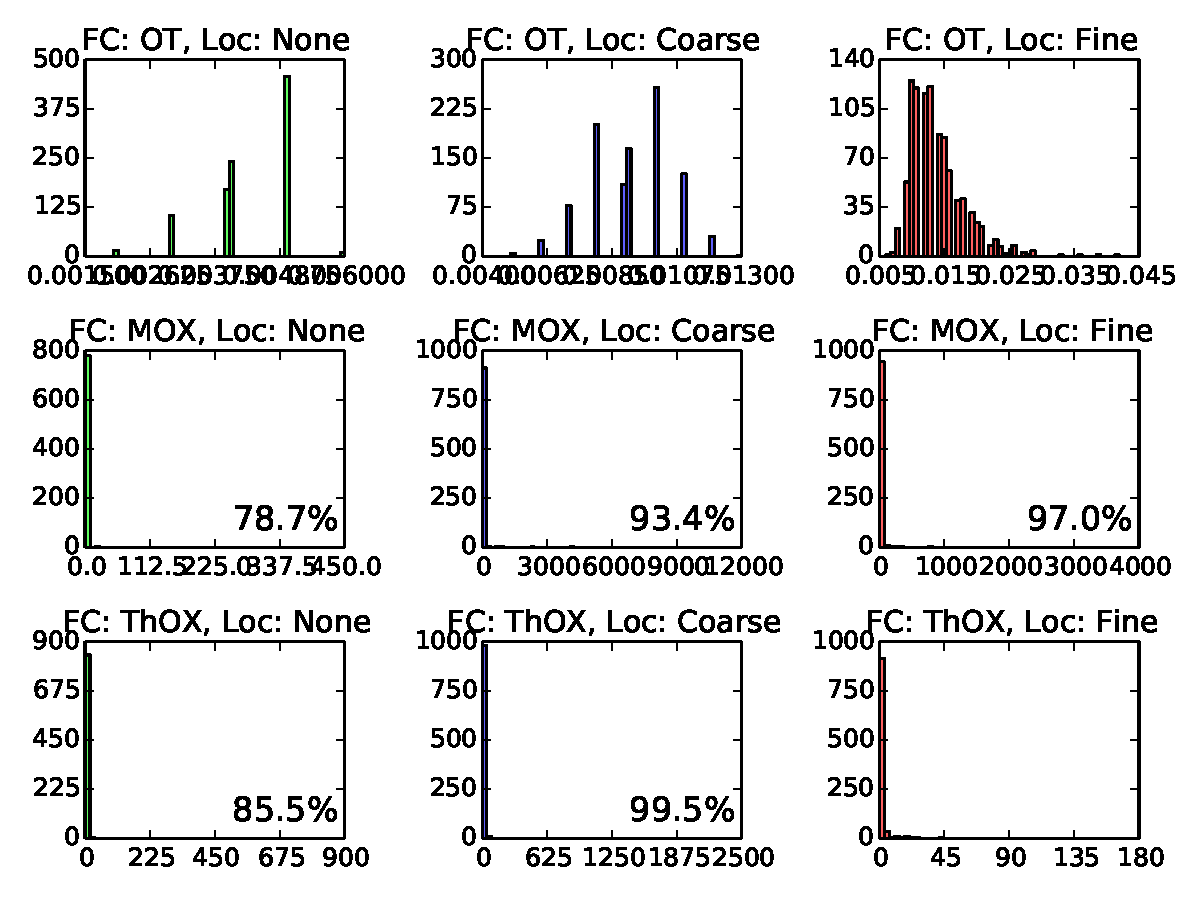
\includegraphics[width=.7\textwidth]{1k_hist_back_rx0.pdf}
%%     \caption{
%%       \label{fig:1k_hist_back_rx0}
%%       Caption.}
%%   \end{center}
%% \end{figure}

%% \begin{figure}[h!]
%%   \begin{center}
%%     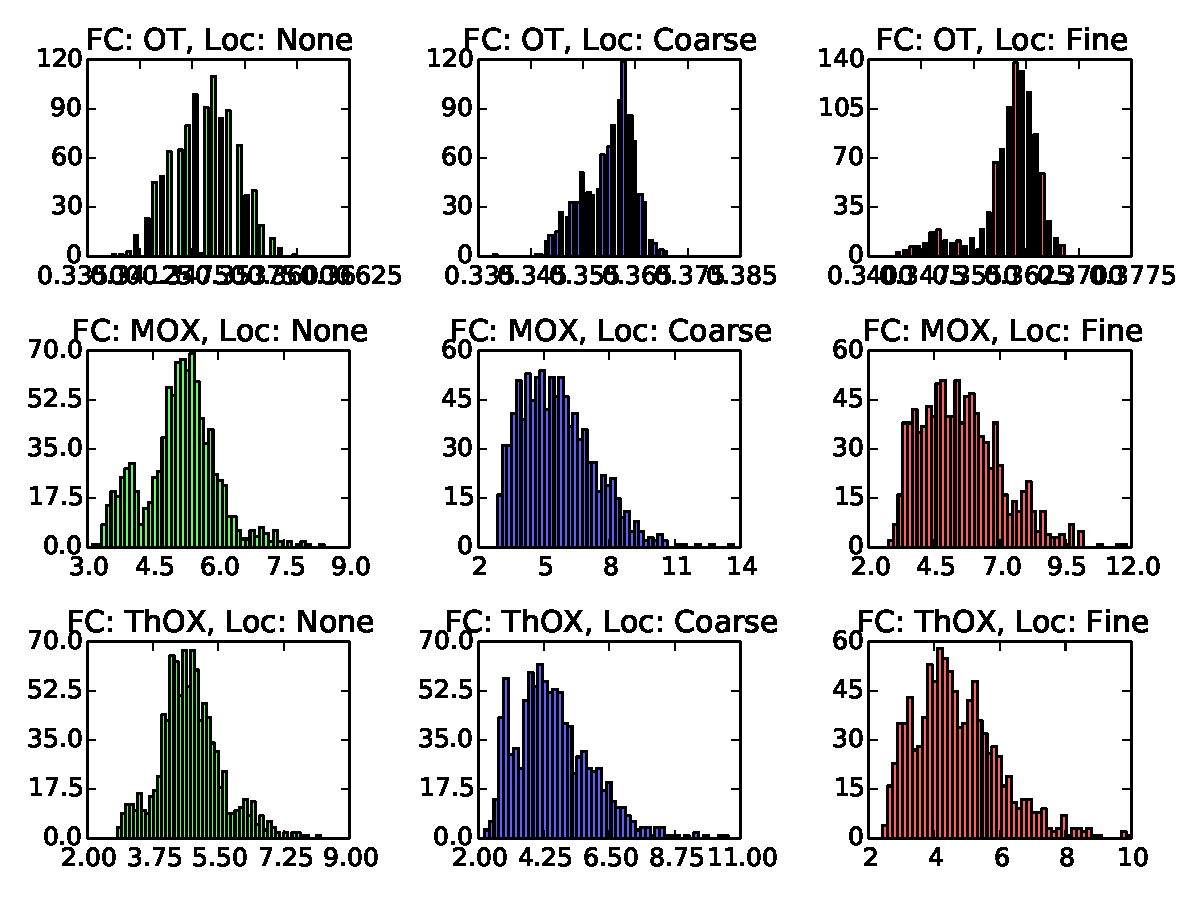
\includegraphics[width=.7\textwidth]{1k_hist_back_rx1.pdf}
%%     \caption{
%%       \label{fig:1k_hist_back_rx1}
%%       Caption.}
%%   \end{center}
%% \end{figure}

%% In the back-end case, lower-fidelity reactor models provide better
%% simulation-based metrics when using the \cbc solver. The higher-fidelity models
%% still maintain a better objective in cost space. This behavior is not reversed
%% for all fuel cycles when moving to a lower artificial-arc cost, suggesting that
%% the model is sensitive to the preference-to-cost translation function.

%% \begin{figure}[h!]
%%   \begin{center}
%%     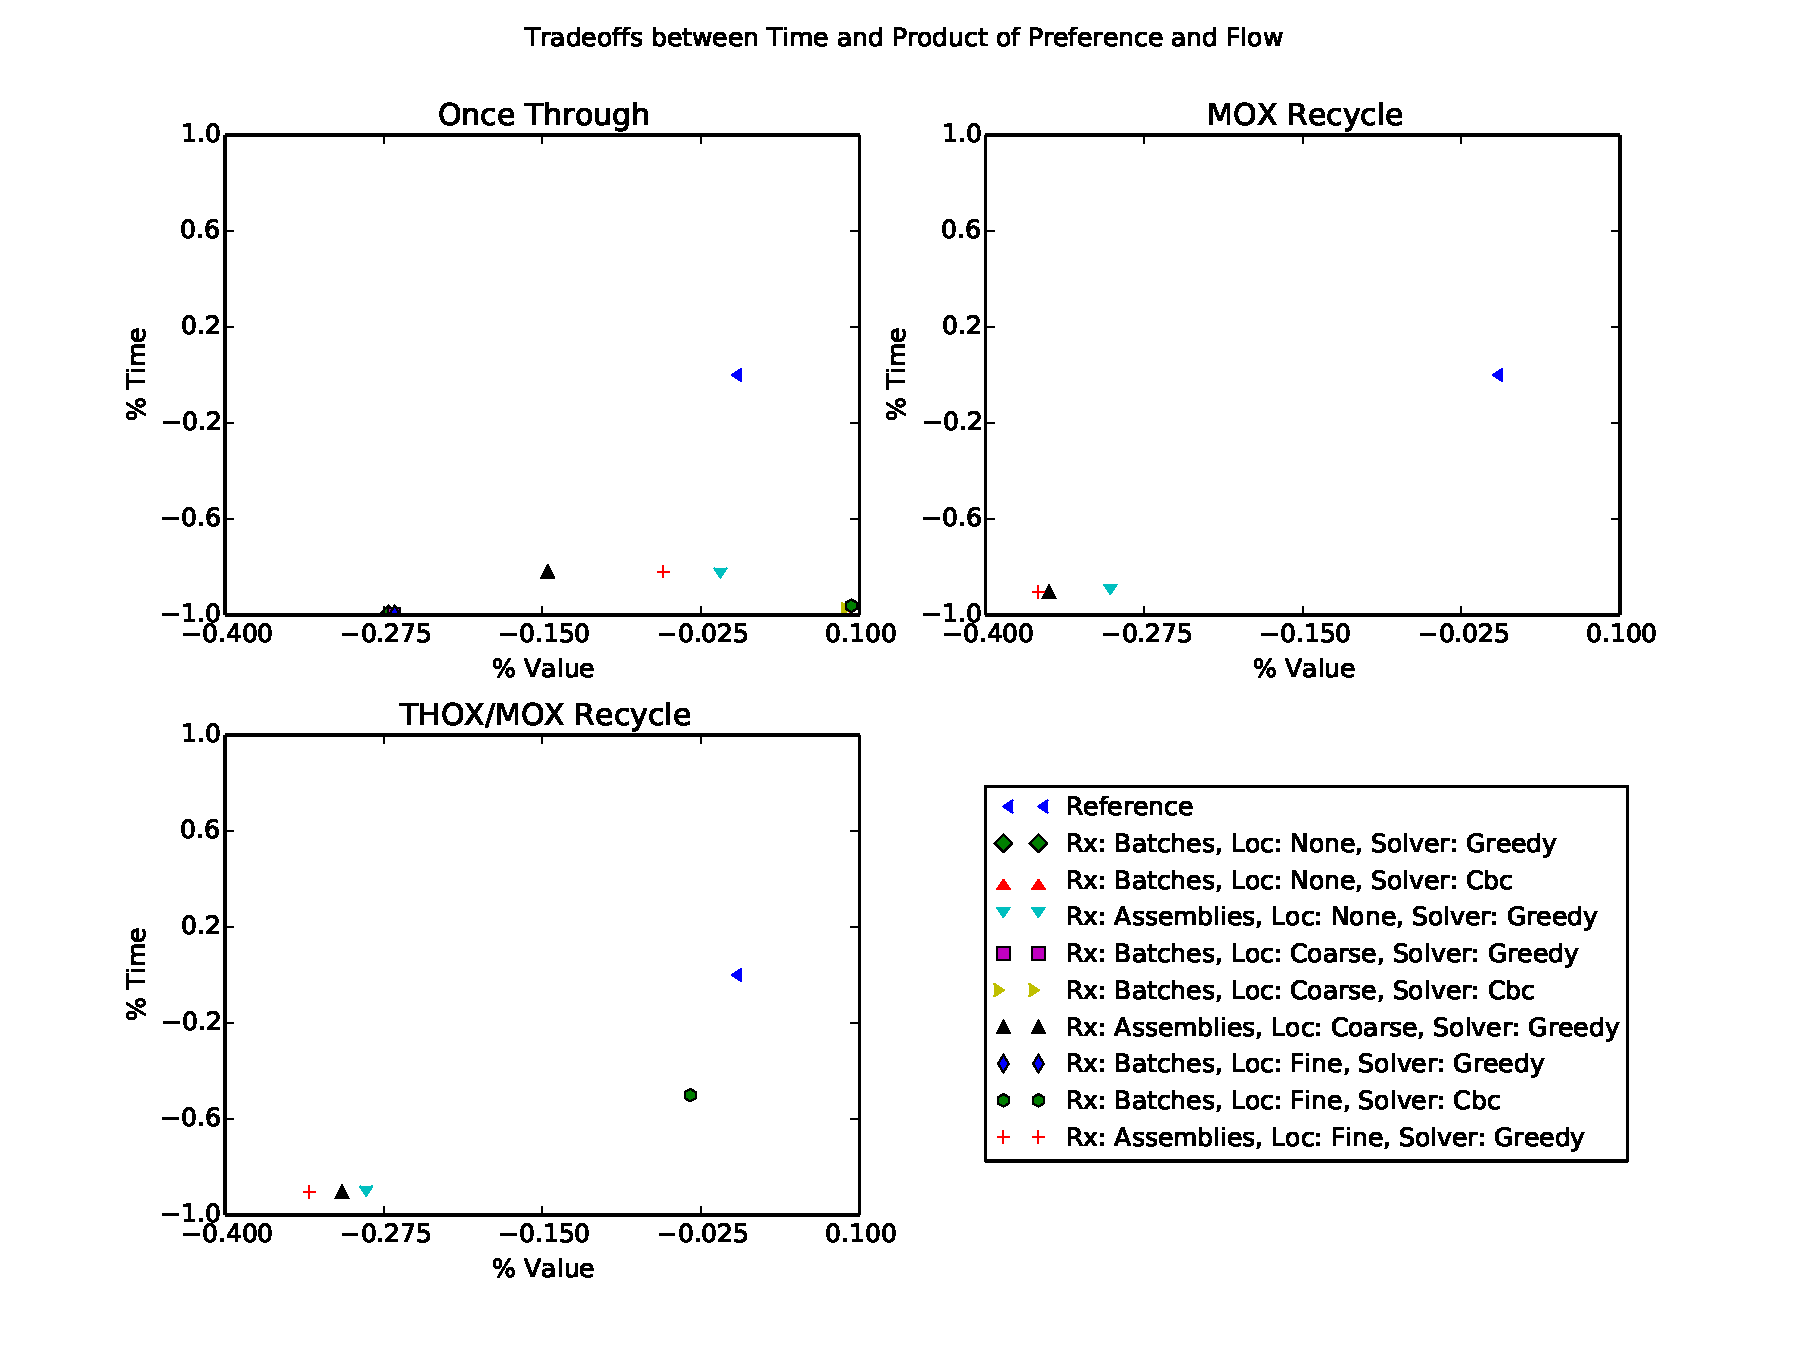
\includegraphics[width=.7\textwidth]{1k_compare_back_pref_flow.pdf}
%%     \caption{
%%       \label{fig:1k_compare_back_pref_flow}
%%       Caption.}
%%   \end{center}
%% \end{figure}

%% \subsubsection{Preference Conditioning Effects}

%% In some cases, having a small or large location-based preference showed
%% significant performance effects. 

%% \begin{figure}[h!]
%%   \begin{center}
%%     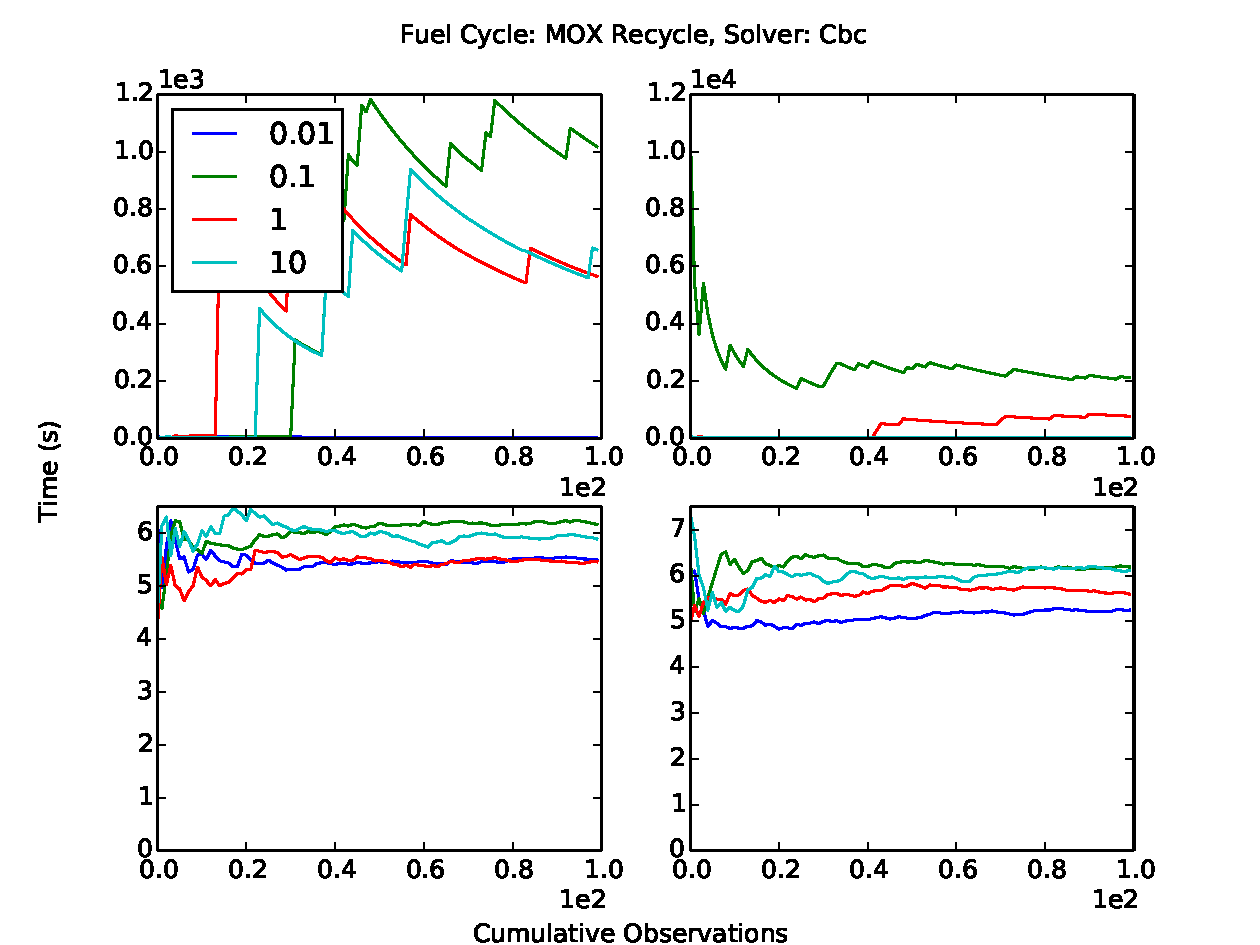
\includegraphics[width=.7\textwidth]{rlc_avg_back_time_fc1_cbc.pdf}
%%     \caption{
%%       \label{fig:rlc_avg_back_time_fc1_cbc}
%%       Caption.}
%%   \end{center}
%% \end{figure}

%% With a small location preference value, preference flows are effectively unaltered.

%% \begin{figure}[h!]
%%   \begin{center}
%%     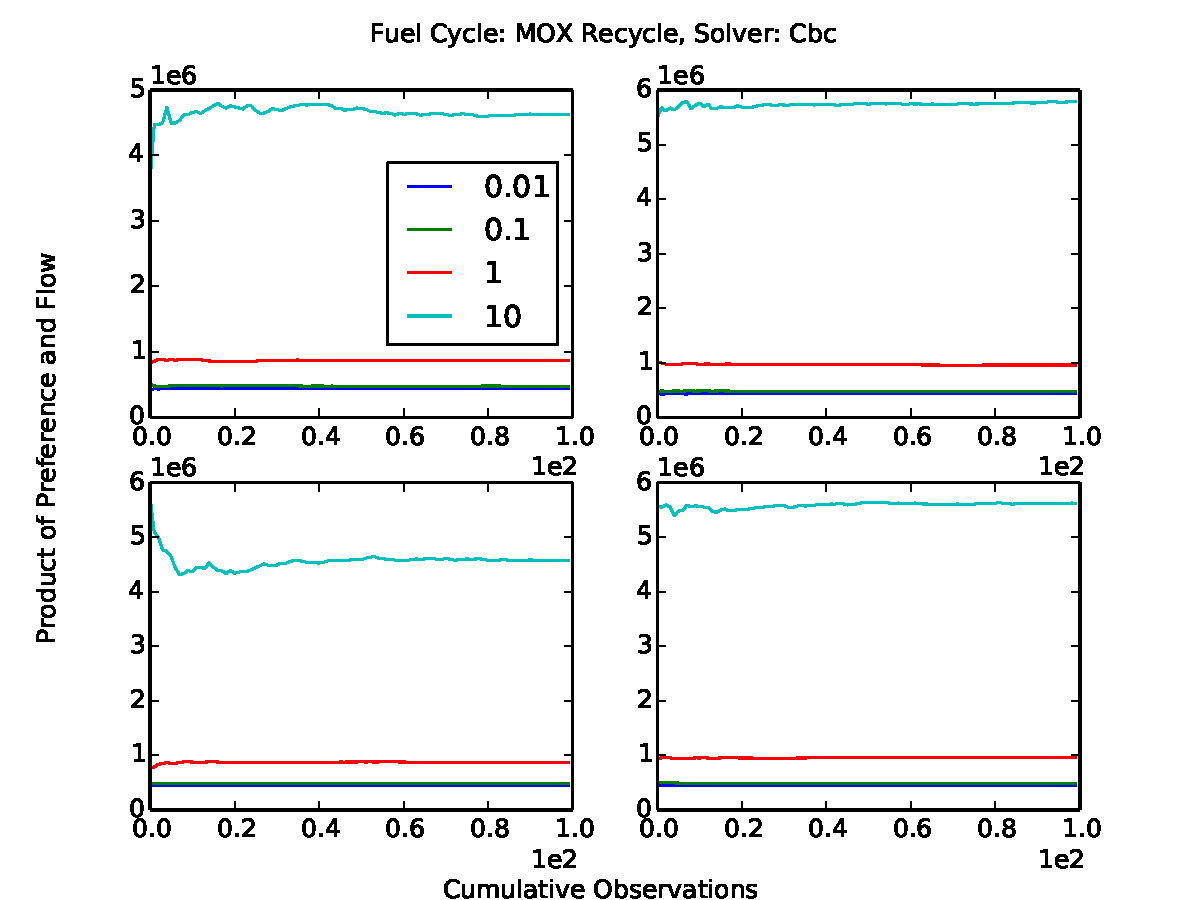
\includegraphics[width=.7\textwidth]{rlc_avg_back_pref_flow_fc1_cbc.pdf}
%%     \caption{
%%       \label{fig:rlc_avg_back_pref_flow_fc1_cbc}
%%       Caption.}
%%   \end{center}
%% \end{figure}


